\documentclass[oneside, titlepage]{scrartcl}

\usepackage[letterpaper, margin=1in]{geometry}
\geometry{letterpaper}
\usepackage{graphicx}

\usepackage{authblk}
\usepackage{amsmath}
\usepackage{amssymb}
\usepackage[hidelinks]{hyperref}
\usepackage{mdwlist}
\usepackage[font=small,labelfont=bf]{caption}
\usepackage{placeins}
\usepackage{subcaption}
\usepackage{tgpagella} \renewcommand{\bfdefault}{bx}

\title{Linear Algorithms for Determining High-Coverage Backbones in Wireless Sensor Networks}
\author{Arya D. McCarthy\\\texttt{\href{mailto:admccarthy@smu.edu}{admccarthy@smu.edu}}}
\affil{Southern Methodist University}
\date{December 15, 2015}							% Activate to display a given date or no date

 \renewcommand{\abstractname}{Introduction and Summary}

\begin{document} %%%%%%%%%%%%%%%%%%%%%%%%%%%%%%%%
\maketitle
%\section{}
%\subsection{}

\tableofcontents
\newpage

\section{Executive Summary}
\subsection{Introduction and Summary}
Wireless sensor networks (WSNs) are intercommunicating sensors spread across a geographic region to monitor and relay information. They have applications for  military, industry, and the general market. A model of a WSN spread across a plane could represent the \emph{nodes} (individual constituents of the WSN) across a constrained geographic region, while a model distributed across a sphere could model a WSN spread worldwide. 

Since we consider coverage of such sweeping geographic regions, it is costly (and for some applications, dangerous) to perfectly position nodes in some regular pattern. Instead, we imagine nodes randomly distributed, as if dropped from an airplane over the area of interest. Each node has a limited range over which it can communicate, so we can model the networks with a \emph{random geometric graph}. These assume that, over the spatial region, some $n$~nodes are uniformly and independently positioned. After that, if nodes are within a distance~$r$ of each other, we create an edge between them. This edge, in our case, shows which nodes can communicate with each other. Recognizing these connections is important to routing data through the WSN and assigning frequencies to reduce interference and energy consumption. A minimal set of nodes for maximizing coverage is called a \emph{backbone}.

This report outlines a fast method of identifying backbones, implementing graph coloring (which can represent frequency allocation to minimize interference: neighboring nodes should transmit on different frequencies, represented as colors) that relies on the smallest--last ordering strategy.

The distinct color groups are independent sets; two of these combined form a bipartite subgraph. This subgraph makes a backbone: a top--level communication line for hierarchically structuring the network. Nodes in each independent set cannot communicate with one another directly, so the other set links them together to achieve maximum coverage of the area of interest.

The implementation provided here is multiplatform because it is written in Python, rather than a compiled language. It efficiently computes the edge sets for random geometric graphs using $k$-d trees, which are designed for spatial partitioning. Further, the smallest--last ordering and coloring occur in $O(|V| + |E|)$ time because of the use of a table of degrees and copious use of hash--based data structures. It also avoids the typical space bloat of Python programs by using generators when possible, yielding one item at a time rather than computing and allocating an entire list that may not be used. Finally, the tool relies on only packages freely available through the default Python package installer, so there are no licensing fees or intellectual property concerns. 

Each of 12 benchmark graphs is included, visualized, with this report, along with a plot of degrees in the smallest--last ordering, the size of each color group for coloring, and graphs of the bipartite backbones. \autoref{tab:rggs} describes the properties of each test case. \autoref{table:color} summarizes the results of coloring each RGG. \autoref{table:bipartite} shows the attributes of the two largest bipartite backbones.
% TODO: references
\subsection{Programming Environment Description}
\subsubsection{System}
A table of the computer's specifications is provided in \autoref{table:system}. A screenshot of the device's built--in display of properties is shown in \autoref{fig:system}.
\begin{table}[h!]
\centering
\begin{tabular}{l | l}
\textbf{Aspect} & \textbf{Description} \\
\hline
Computer & Apple MacBook Pro (13-inch, Late 2013)\\
Operating system & Mac OS X, Version 10.11.2 (build 15C50) \\
Processor & 2.4 GHz Intel Core i5, dual--core \\
Memory & 8 GB \\
\end{tabular}
\caption{Relevant system attributes, summarized}
\label{table:system}
\end{table}

\begin{figure}[h!]
\centering
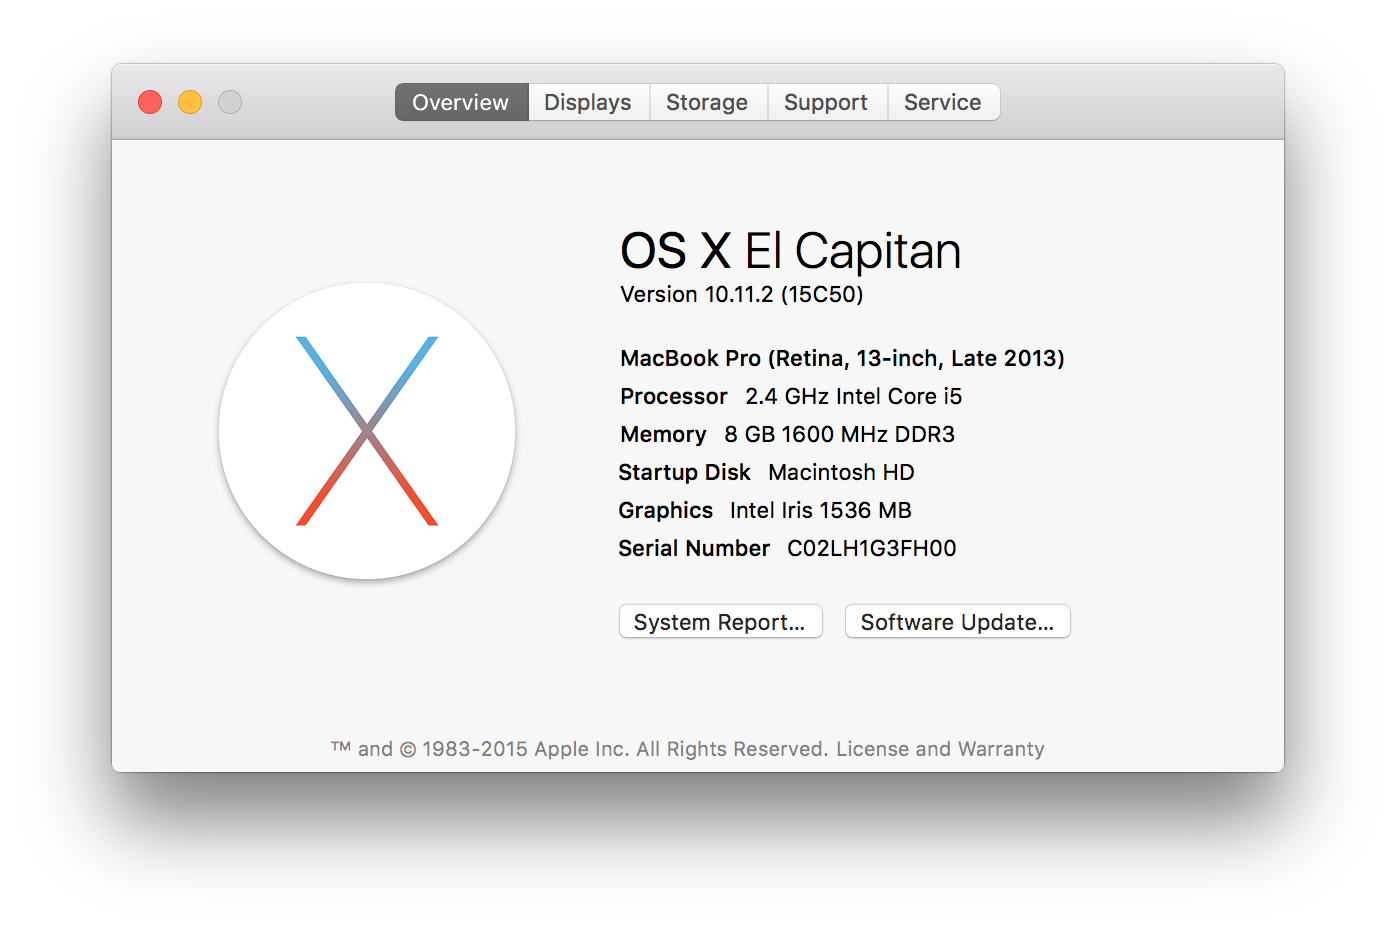
\includegraphics[width=0.8\textwidth]{figures/device_environment}
\caption{Relevant system attributes, according to device}
\label{fig:system}
\end{figure}

\subsubsection{Language and libraries}
I used Python for this project---particularly, CPython 2.7.10, compiled using LLVM 7.0.

Though Python comes with many standard packages, some nonstandard packages were used to prepare this report. NetworkX, originally developed by Los Alamos National Laboratory, defines an adjacency-list--backed Graph class and a rich API for manipulating it [6]. SciPy contains an implementation of $k$--d trees, which can efficiently compute a node's neighbors in space [11]. The matplotlib library provides tools for plotting and data visualization, modeled after Matlab's built--in tools [7]. These plots can be dragged, rotated, and scaled.

This report was prepared using \LaTeX, and the document compiler wound up having a higher memory requirement than this project's peak resource consumption (1.97 GB vs 1.68 GB). Considering Python's pointer--based object structure, this is a reasonable resource allocation, brought about by some optimizations to be explained below. The time to compute and plot all relevant attributes for the largest required benchmark was 6 minutes, 42 seconds. Implementations in other languages may improve on this, by compiling code instead of interpreting and by minimizing pointer dereference.

\subsection{References}
\begin{enumerate*}
\item
A. Kosowski, K. Manuszewski, Classical Coloring of Graphs, Graph Colorings, 2-19, 2004. ISBN 0-8218-3458-4.
\item
R.M. Karp, "Reducibility Among Combinatorial Problems", Complexity of Computer Computations. New York: Plenum. pp. 85--103. 1972.
\item
D.W. Matula, Wireless Sensor Network Project, \url{www.lyle.smu.edu/cse/7350/}, 2015
\item
D.W. Matula , L.L. Beck, ``Smallest-last ordering and clustering and graph coloring algorithms'', Journal of the ACM (JACM), v.30 n.3, p.417-427, July 1983.
\item
M.D. Penrose: Random Geometric Graphs (Oxford Studies in Probability, 5), 2003.
\item
NetworkX Library, v1.10, \url{https://networkx.github.io}, 2015
\item
matplotlib Library, v1.3.1, \url{http://matplotlib.org}, 2015
\item
NetworkX Random Geometric Graph implementation using K-D trees, \url{http://stackoverflow.com/questions/13796782/networkx-random-geometric-graph-implementation-using-k-d-trees}, 2015
\item
Z. Chen, Wireless Sensor Network Project, \url{http://lyle.smu.edu/~zizhenc/file/Wireless\%20Sensor\%20Network.pdf}
\item
$k$--d Tree, \url{https://en.wikipedia.org/wiki/K-d_tree}, 2015
\item
scipy.spatial.KDTree, \url{http://docs.scipy.org/doc/scipy-0.16.0/reference/generated/scipy.spatial.KDTree.html}, 2015
\end{enumerate*}

\section{Reduction to Practice}
\subsection{Data Structure Design}
Python employs typical language built-ins like integer and boolean types. These are represented, as are all Python data types (with exceptions in some libraries), as pointers to the relevant data. Further, Python has built--in lists backed by arrays, as well as sets and dictionaries backed by hash tables. The uses of these will be explained shortly.

Positions of nodes in space were represented as 2--tuples for disk and square and 3--tuples for sphere (rather than representing spherical coordinates using $\theta$ and $\phi$. This was the data format that matplotlib expected for plotting [7], as well as the format that the SciPy $k$--d tree structure expected points for computing the edge set [11].

Graphs were represented by a pair of structures: a hash table mapping data node IDs onto their properties (in this case, the coordinates for plotting), and more importantly, an adjacency list. Unlike typical adjacency lists, which use lists of lists (either backed by linked lists or arrays), my implementation relied on the Python \texttt{dict(ionary)} structure as a highly tuned hash table implementation. One hash table mapped each node to a hash table (backing a set ADT) of its neighbors. The advantage of hash-based data structures is quick insertion, deletion, and search.

To perform smallest--last ordering, I also created a bucket queue data structure as described in Matula (1983) for tracking degrees. It was structured the same way as my adjacency list: a hash map (from now on, ``dictionary'') mapping degree onto the set of nodes with that degree. The primary advantage of storing the nodes in sets is that removal from arbitrary positions is possible; Python's built--in list is backed by an array, so removing an element is $O(n)$ in the worst case, compared to $O(1)$ for sets. If a linked list were used, removal would be $O(1)$, but lookup would be $O(n)$. This implementation made choices favoring time over space, but the space requirement is still modest on modern consumer hardware.

$k$--d trees are a useful data structure for efficiently partitioning space and for identifying neighbors [10]. The algorithm is related to the cell method for edge identification, so it is used to compute the edge set of each random graph.

\subsection{Algorithm Descriptions}

\subsubsection{Sphere random point generation}

The problems of finding random points in the unit square and disk are trivial, but identifying random points on a sphere presents a challenge that has been studied for decades. To pick spherical coordinates from a uniform distribution would cluster points near the poles. Consequently, numerous equivalent strategies for random point generation have emerged. Many rely on rejection sampling: picking values from a uniform distribution until the values satisfy some criterion necessary for uniformity. The danger here is that there is no guarantee of termination within reasonable time bounds. Others rely on multiple trigonometric functions, each of which requires many CPU cycles. In profiling, the fastest used neither and was presented by Muller: create a vector in $\mathbb{R}$, then normalize it.

\begin{equation}
\frac{1}{\sqrt{x^2 + y^2 + z^2}} \begin{bmatrix} x \\ y \\ z \end{bmatrix}
\end{equation}

For large $n$, this approach produced a 25\% speedup over the next best method.

\subsubsection{Smallest--last vertex ordering}

A smallest--last vertex ordering is an ordering of a graph's vertices $V$ such that each vertex $v_i \in ord_{SL}(V)$ is of minimal degree in the subgraph on only nodes $1$ through $i$. The general procedure involves three steps, repeated until the graph is empty:
\begin{enumerate}
\item
Pick the node of minimal degree.
\item
Remove it from the graph.
\item
Save it to the next empty position in the result ordering.
\end{enumerate}
When all of this has been done, reverse the ordering. This will put the last--removed node first and vice versa. By the end of this period, the procedure has processed every node and deleted every edge; the algorithmic complexity is $O(|V| + |E|)$, and this implementation satisfies that bound [4]. 

Smallest--last ordering is one strategy for node selection in greedy coloring. 

\subsubsection{Greedy coloring}

Once the ordering has been determined, greedy coloring is a swift operation. (Graph coloring is an NP--complete problem [2]; this is a heuristic for approximating the best coloring.) 

The procedure is as follows: for every node in the ordering (in this case smallest--last), identify the set of its neighbors' colors, if they exist. Then find the first color not in that set and assign it to the current node [1]. 

Because each node's neighbors must be a different color, the color class contains no adjacent nodes. This means that each color class is an independent set.

\subsection{Algorithm Engineering}
\subsubsection{Smallest--last vertex ordering}
Two of the three steps identified above are simple. 
\begin{itemize}
\item
Removing a node from the graph would take time proportional to its degree, since we have to remove each of its edges, and the search and remove operations each take constant time because of the hash--based adjacency list. The sum of the degrees is $2|E|$, so the total cost of removal is $O(|V| + |E|)$.
\item
Inserting each node in its correct location in a dynamic array would require $O(|V|^2)$ time since every insertion is at the front, making each of the $|V|$ inserts require $O(|V|)$ time. To improve this bound, I preallocated an array of length $|V|$, then computed the appropriate index for insertion.
\end{itemize} 

However, identifying the node to remove is more challenging. Because the degrees change on each iteration, we cannot simply sort the edges by degree and use that as our ordering. A naive response would be, on every iteration, to scan through the nodes, compute each degree and pick the minimum element. However, this raises the complexity of the algorithm to $O(|V|^2 + |E|)$ because we perform a linear pass on every iteration. For a network of 16,000 nodes, the runtime is nearly three hours. 

Instead, we use the degree table structure I identified before. Begin by bucketing each vertex by degree. Then, when a new node is required, select the smallest--degree bucket and remove any node. Now identify its neighbors using the graph structure. For each of these, move it from its degree bucket to the bucket for $deg-1$. Since we use sets, each of these operations is $O(1)$. We wind up moving nodes through the buckets $|E|$ times, and we would have performed asymptotically as many operations anyway in restructuring the graph. Combined with the explanation from Section 2.2.1, the runtime for this algorithm is still $O(|V| + |E|)$.

Because of the classic tradeoff between time and space, this algorithm does not achieve optimal space bounds. The degree table has size $O(|V|)$, whereas the naive selection method explained above would require only constant space for smallest--node identification. 

\subsubsection{Greedy coloring}
The cleverness in the coloring scheme mostly comes from using sets to track neighbors' colors and the color assigned to each node. Order doesn't matter, and there will be no duplicate nodes. This way, we can check whether the neighbor is colored in $O(1)$ time and find the next free color in $O(k)$ time, where $k$ is the total number of colors used. Restating, we iterate over each node to color it, performing work equal to the node's degree. The sum of the work on degrees is $O(|E|)$, so the total work is $O(|V| + |E|)$.

\subsection{Verification Walkthrough}
We will now walk through my techniques on a small graph, with $n = 20$ and $r = 0.40$. First, we see the graph itself in \autoref{fig:verification:graph}. A max--degree node and its edges are in red; a min--degree node and its edges are in blue.

\begin{figure}[h!]
\centering
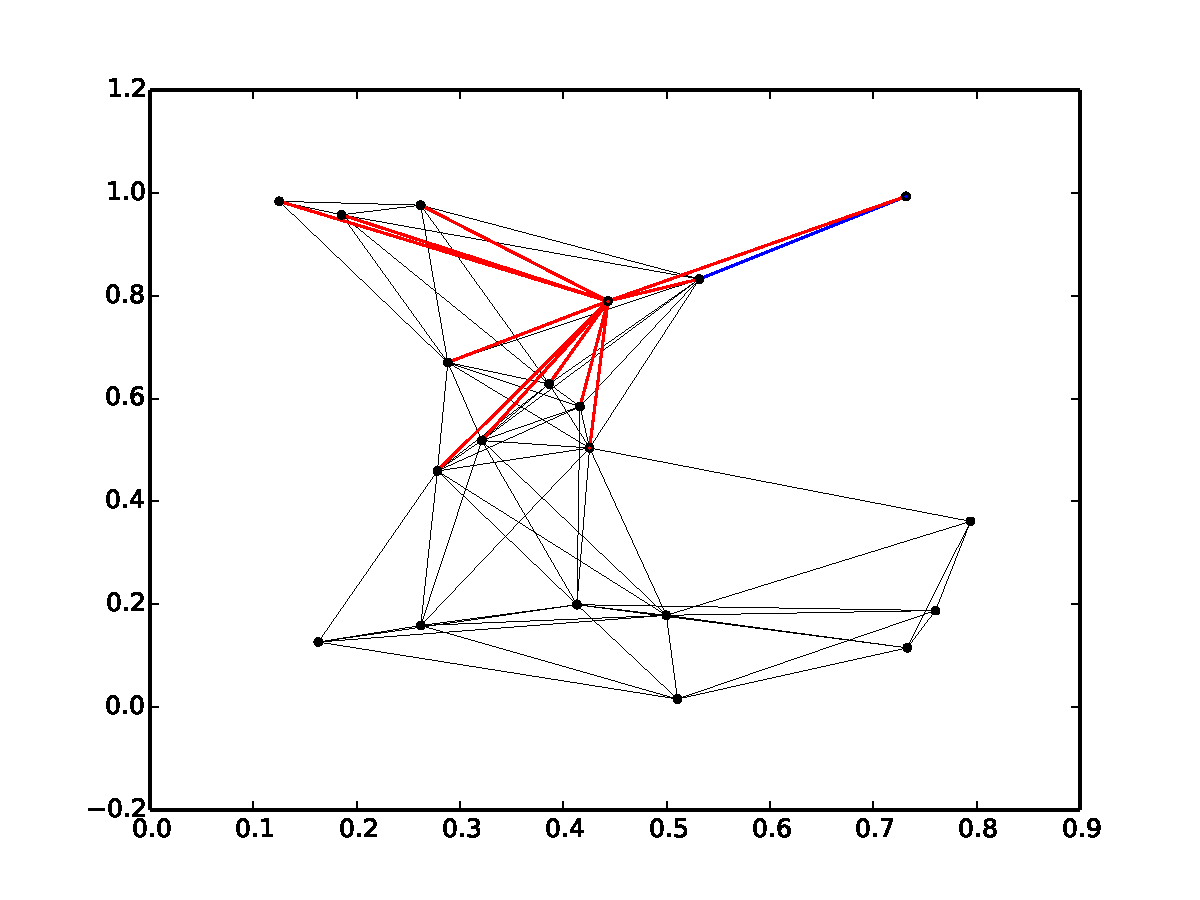
\includegraphics[width=0.8\textwidth]{figures/graph100.pdf}
\caption{A random graph $G(N=20, R=0.40)$. The nodes of min and max degree are highlighted, along with their edges, in blue and red, respectively.}
\label{fig:verification:graph}
\end{figure}

Next, we perform the smallest--last ordering. A walkthrough is provided in \autoref{fig:verification:coloring}, numbering each node in order of removal and displaying the resultant coloring. For instance, node 18 is the node of minimal degree at the beginning, so it is removed from the graph and added to the end of our smallest--last list. This reduces the degree of nodes 7 and 14. Next, there are multiple nodes with degree 4 in the remaining graph. Each is equal, so we remove node 8 arbitrarily, reducing the degree of nodes 4, 6, 10, and 12. The process repeats. Eventually, we reach the state of having seven nodes with degree 6. This is the terminal clique; we can remove these nodes in any order and the clique property is maintained. Eventually, every node is removed.

\begin{figure}[h]
\centering
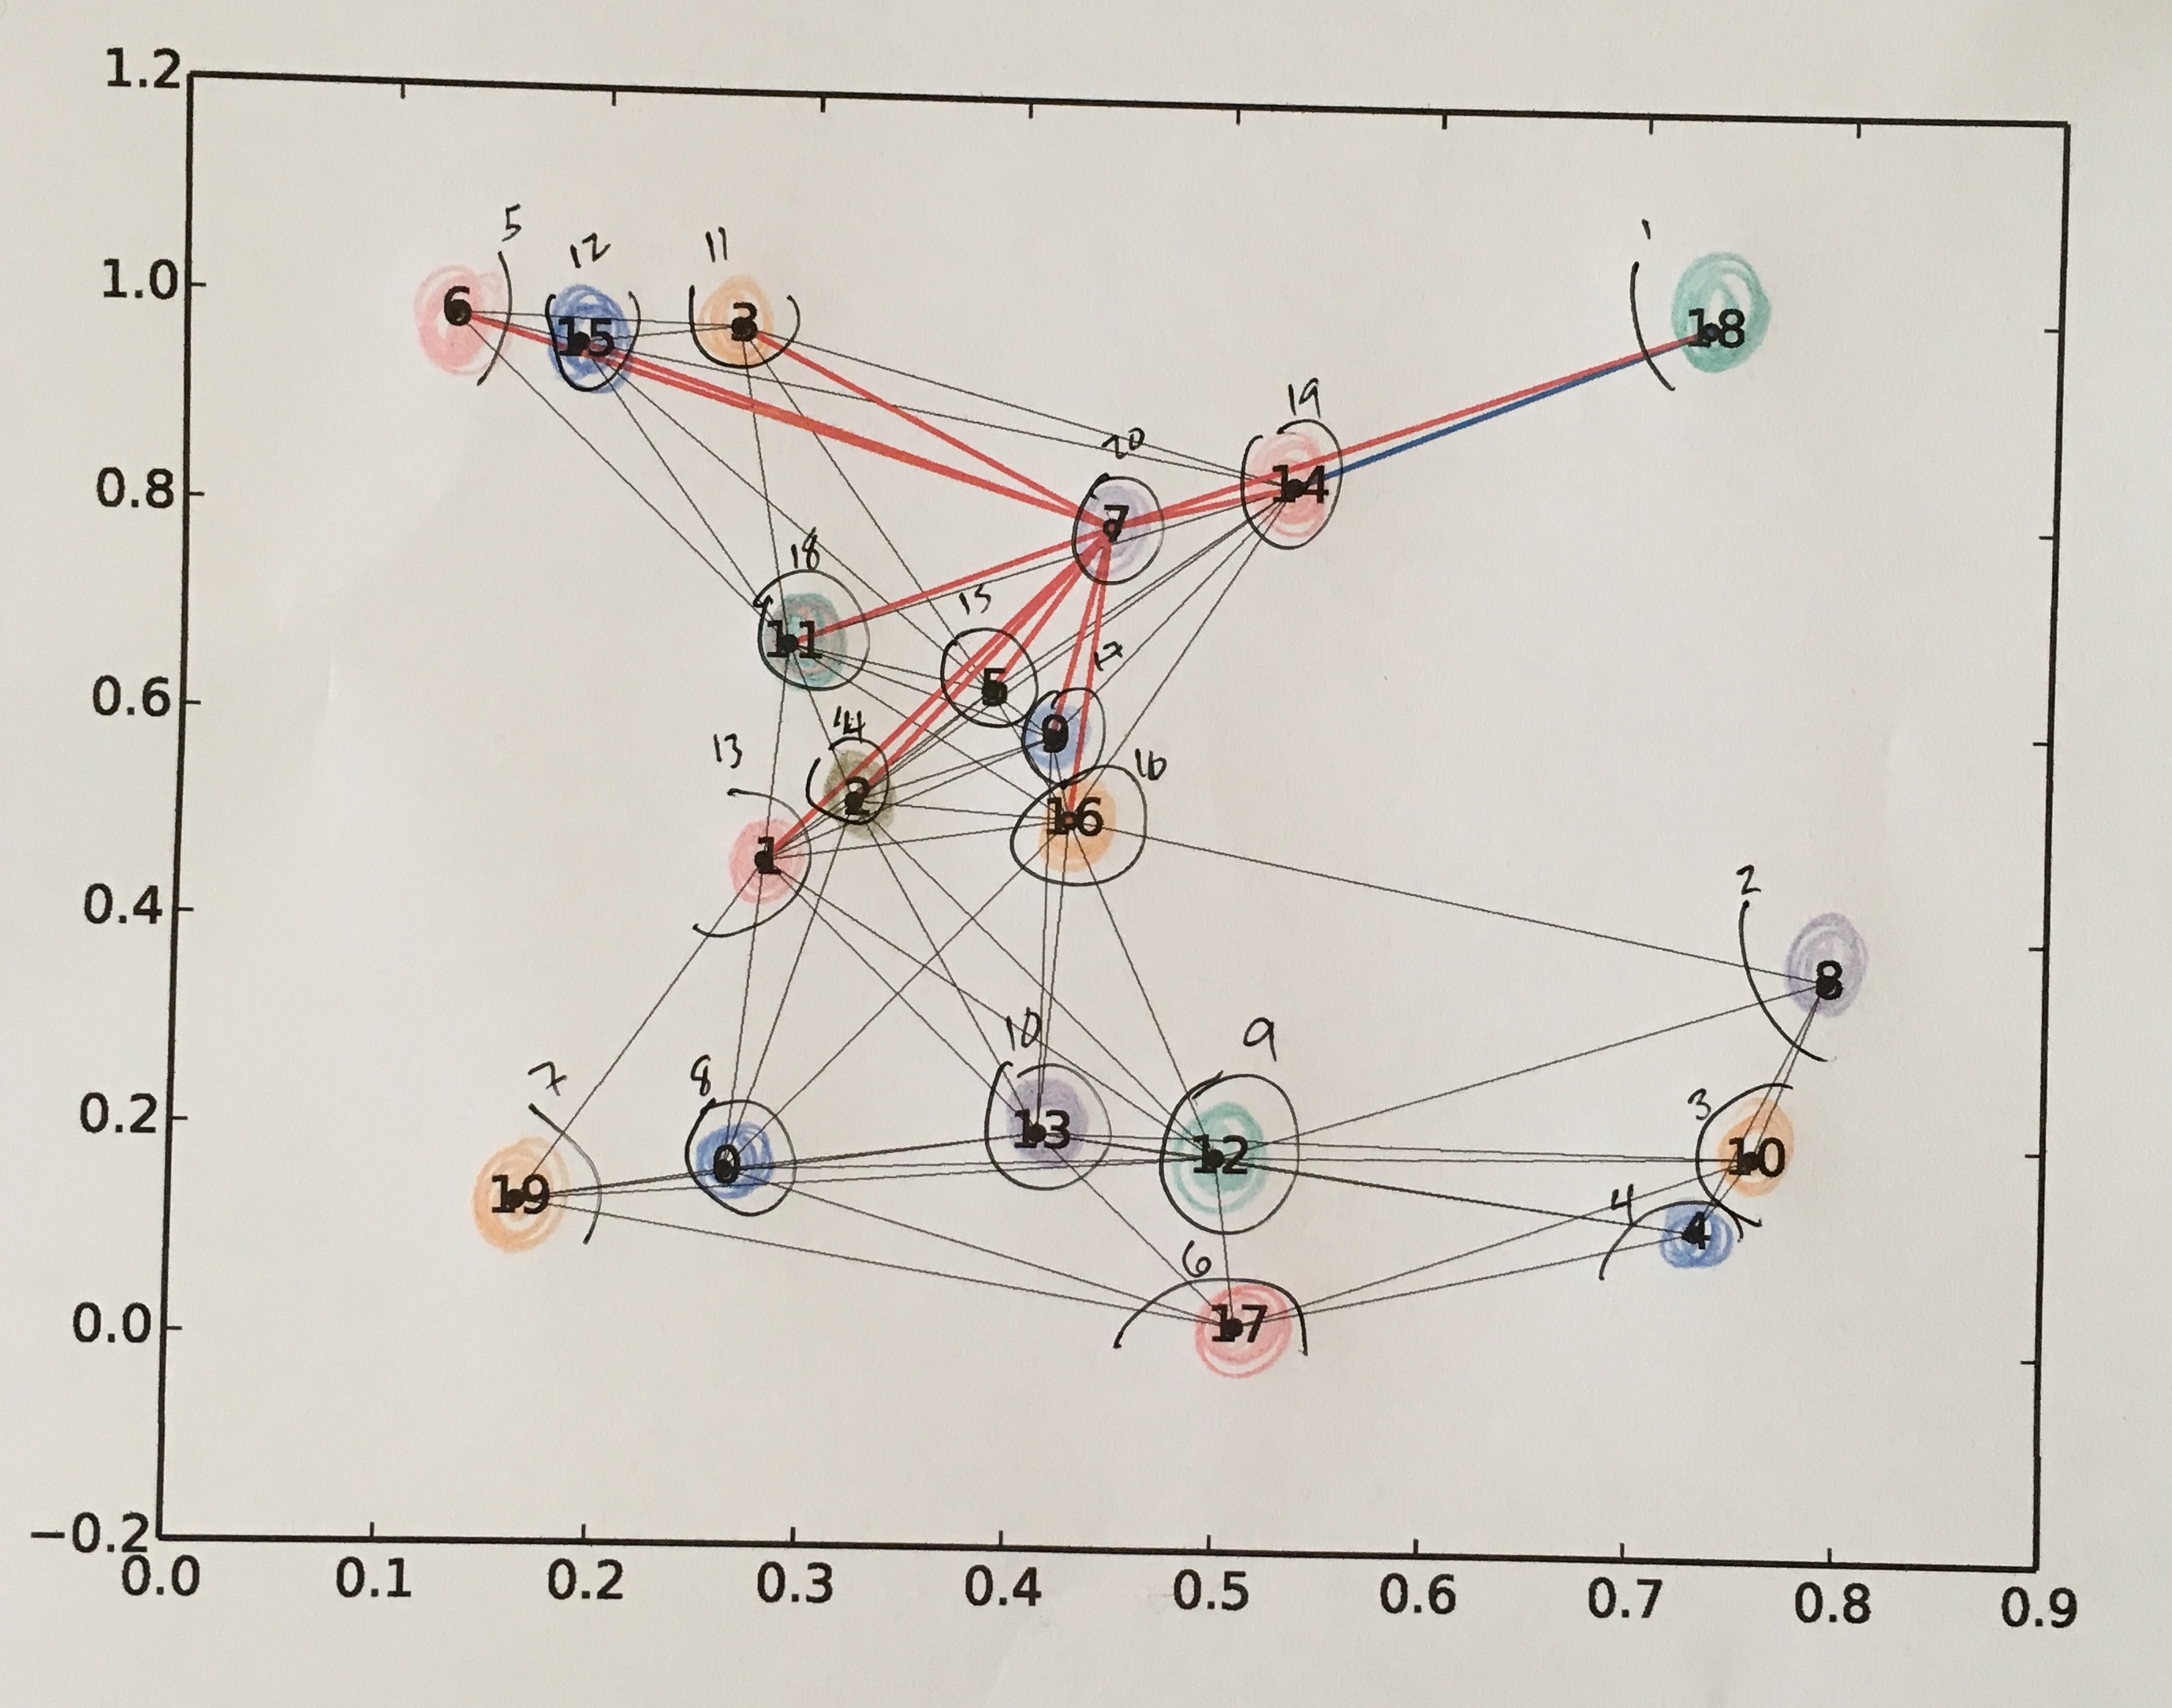
\includegraphics[width=0.8\textwidth]{figures/handdone.JPG}
\caption{Coloring and smallest--last removal for $G(N=20, R=0.40)$.}
\label{fig:verification:coloring}
\end{figure}

\autoref{fig:verification:degree} is also a graph of the degree when removed. Note that, as a sanity check, the degree never exceeds the true degree of the node.

\begin{figure}[h!]
\centering
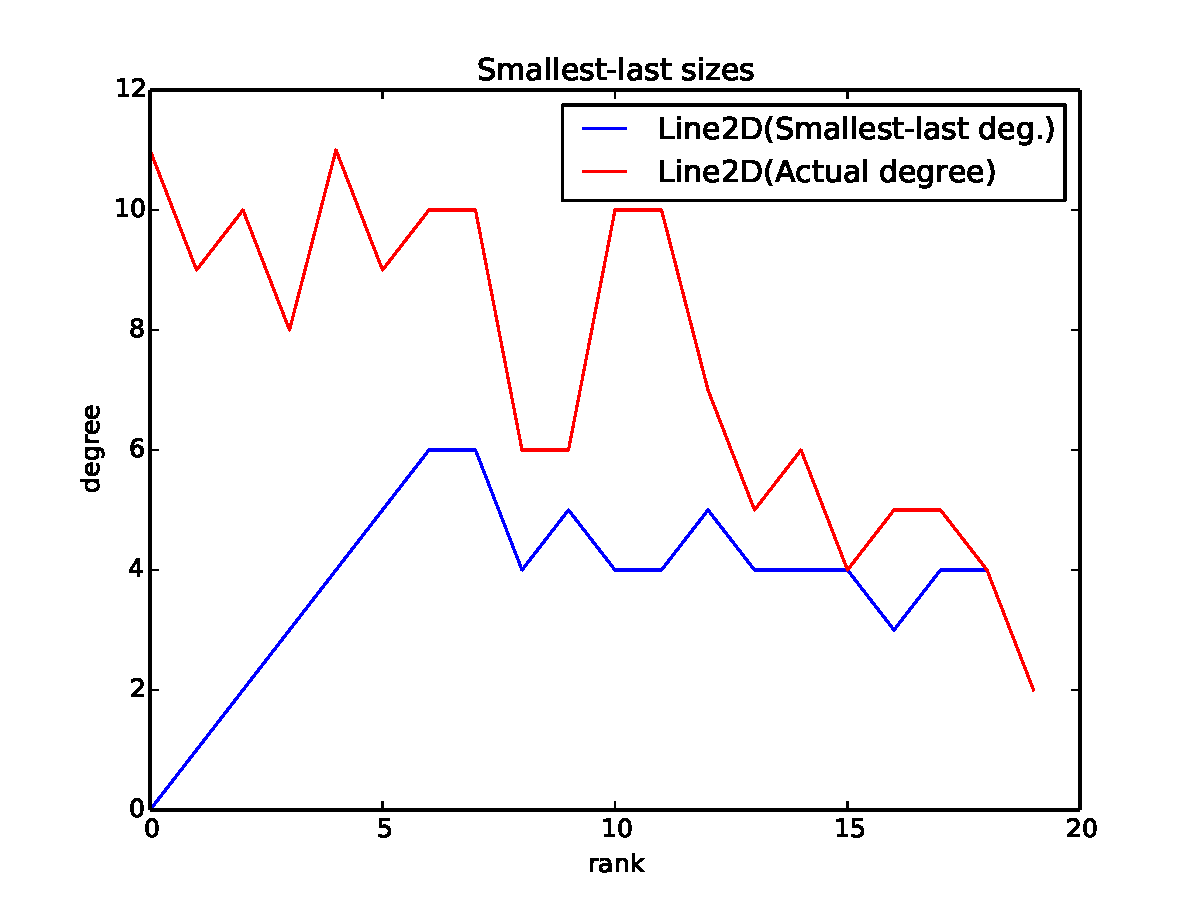
\includegraphics[width=0.8\textwidth]{figures/ordering100.pdf}
\caption{Smallest--last sizes for each node, compared to actual degree of each node}
\label{fig:verification:degree}
\end{figure}


We determine the backbone by comparing the independent sets' sizes and choosing the one with the largest number of edges. It's seen here; the thicker black lines represent the backbone.

\begin{figure}[h!]
\centering
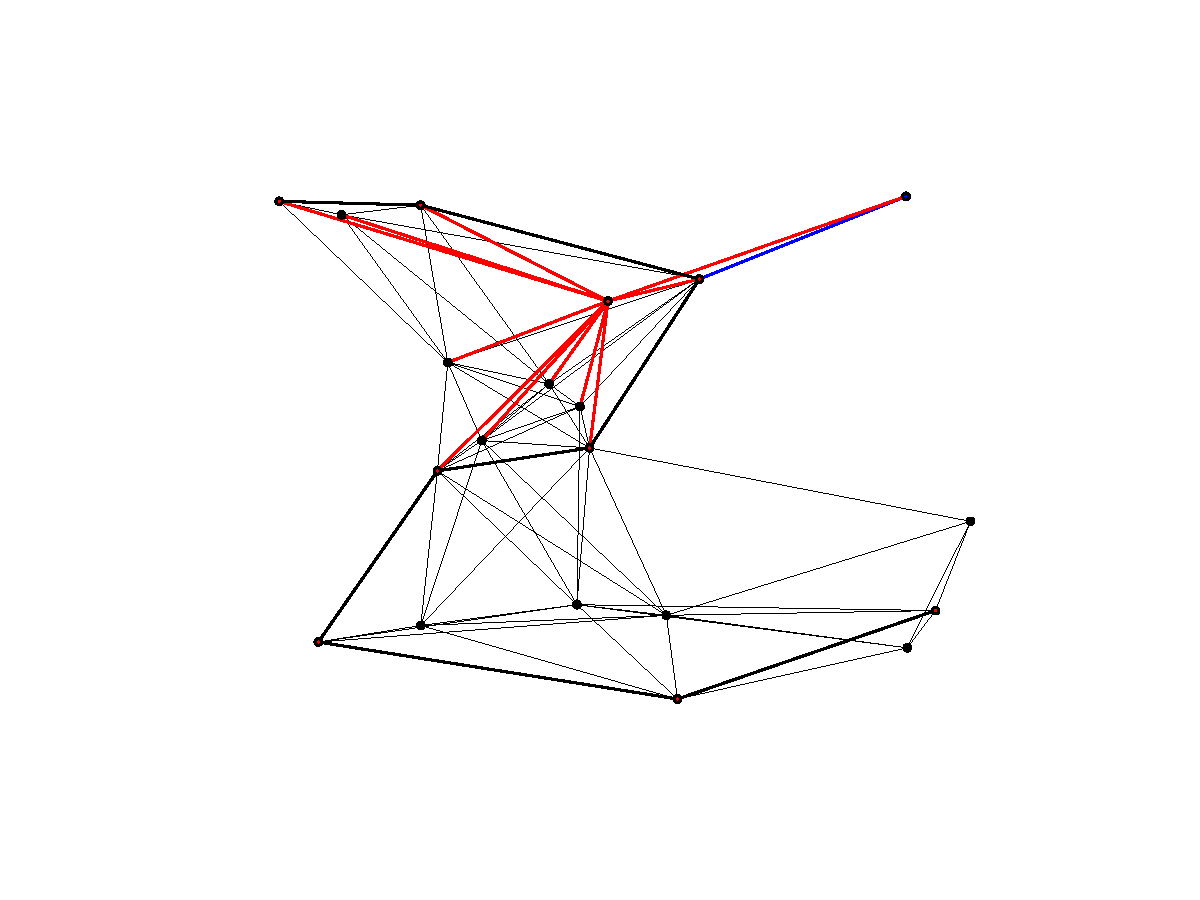
\includegraphics[width=0.8\textwidth]{figures/simplegraph100.pdf}
\caption{The backbone for this 20--node graph is shown in thick black lines. The nodes of min and max degree and their edges are still shown in blue and red, respectively.}
\end{figure}


\subsection{Algorithm Effectiveness}
Each of 13 benchmark graphs is included, visualized, with this report, along with a plot of degrees in the smallest--last ordering, the size of each color group for coloring, and graphs of the bipartite backbones. \autoref{tab:rggs} describes the properties of each test case. \autoref{table:color} summarizes the results of coloring each RGG. \autoref{table:bipartite} shows the attributes of the two largest bipartite backbones.

I've previously elaborated on the bounds for these techniques---most importantly, that graph coloring is NP--complete, so we use a greedy heuristic. Also, my use of $k$-d trees for graph generation is an improvement on the quadratic naive solution. My implementation is slow because it is interpreted and because it is implemented in a language in which even integer access requires pointer dereference. Having profiled my implementation another source of slowness in my implementation is that many NetworkX functions require the list of edges, which must be computed from the adjacency list [6].

Based on the times from this test, my algorithm functions well, even for high $|E|$, though I run out of memory with large $|V|$---Python is not a space--efficient language.

\section{Result Summary}

Since results are largely philosophically similar from graph to graph, we will explain properties of the graph from benchmark 1 only. The principles apply across all graphs.

\subsection{Random geometric graph generation}
\autoref{tab:rggs} describes the random geometric graphs used for benchmarking. In the related figures, nodes of max degree and their edges are red. Nodes of min degree and their edges are blue. As requested in the project brief, if the true average degree is $> 30$, I have opted not to draw all edges. In the visualization of graph 1, we see a node of minimum degree on the lower left, colored in blue. On the upper right, there are three nodes of maximum degree; their edges are colored.

The degree histogram for this graph shows that the mode size is 28; nearly 70 nodes have this size. The distribution peaks there and falls off on each side; it is also left--skewed.
\begin{table}[h]
\small
\centering
\begin{tabular}{r r r l | r r r}
$B$ & $N$ & $A_{est}$ & $T$ & $M$ & $R$ & $A_{real}$ \\
\hline
1 & 1000 & 30 & Square & 13672 & 0.0977 & 27.34\\
2 & 4000 & 40 & Square & 76156 & 0.0564 & 38.08\\
3 & 4000 & 60 & Square & 113046 & 0.0691 & 56.52\\
4 & 16000 & 60 & Square & 465952 & 0.0345 & 58.24\\
5 & 64000 & 60 & Square & 1890070 & 0.0173 & 59.06\\
6 & 4000 & 60 & Disk &114346 & 0.122 & 57.17\\
7 & 4000 & 120 & Disk & 221584 & 0.173 & 110.79\\
8 & 4000 & 60 & Sphere & 119933 & 0.245 & 59.97\\
9 & 16000 & 120 & Sphere & 960127 & 0.173 & 120.01\\
10 & 64000 & 120 & Sphere & 3839951 & 0.0866 & 120.00\\
11 & 100000 & 60 & Square & 2964373 & 0.0138 & 59.29\\
12 & 256000 & 60 & Square & 7619381 & 0.00764 & 59.52\\
13 & 1000 & 200 & Square & 80237 & 0.252 & 160.47\\
\end{tabular}
\caption{A summary of the attributes of created random geometric graphs. B = benchmark ID. N = number of sensors. $A_{est}$  = estimated average degree. T = graph type. M = number of pairwise sensor adjacencies (edges). R = distance bound for adjacency. $A_{real}$ = average degree.}
\label{tab:rggs}
\end{table}

\subsection{Graph coloring}
See \autoref{table:color}. In the plots of sequential coloring, note that the degree when extracted never exceeds the original degree, providing a sanity check.

Further, we can see the terminal clique size in the plot for the first benchmark: 18. Once there are 19 nodes left, all have the same degree: one minus the number of nodes. This means that the graph is complete and a clique of size 19.

For graph 1, the color class sizes dropped off quickly after the first few. 

\begin{table}[h]
\small
\centering
\begin{tabular}{r r r l | r r r r r r r r}
$B$ & $N$ & $R$ & $T$ & $M$ & $\Delta_{min}$& $\Delta_{avg}$ & $\Delta_{max}$ & $\Delta min_{max}$ & $k$ & $S$ & $TCS$\\
\hline 
1 & 1000 & 0.0977 & Square & 13672 & 9 & 27.34 & 45 & 20 & 21 & 81 & 18 \\
2 & 4000 & 0.0564 & Square & 76156 & 9 & 38.07 & 61 & 25 & 25 & 242 & 24\\
3 & 4000 & 0.0691 & Square & 113046 & 18 & 56.52 & 86 & 35 & 33 & 174 & 31\\
4 & 16000 & 0.0345 & Square & 465952 & 11 & 58.24 & 94 & 40 & 30 & 678 & 36\\
5 & 64000 & 0.0173 & Square & 1890070 & 14 & 59.06 & 90 & 40 & 38 & 2685 & 37\\
6 & 4000 & 0.122 & Disk & 114346 & 19 & 57.17 & 83 & 35 & 33 & 176 & 32\\
7 & 4000 & 0.173 & Disk & 221584 & 41 & 110.79 & 158 & 63 & 57 & 96 & 49\\
8 & 4000 & 0.245 & Sphere & 119933 & 32 & 59.97 & 85 & 37 & 35 & 168 & 34\\
9 & 16000 & 0.173 & Sphere & 960127 & 79 & 120.01 & 156 & 80 & 63 & 359 & 52\\
10 & 64000 & 0.0866 & Sphere & 3839951 & 79 & 120.00 & 162 & 81 & 63 & 1435 & 53\\
11 & 100000 & 0.0138 & Square & 2964373 & 15 & 59.29 & 91 & 39 & 38 & 4189 & 35\\
12 & 256000 & 0.00864 & Square & 7619381 & 17 & 59.52 & 94 & 41 & 39 & 10684 & 36\\
13 & 1000 & 0.252 & Square & 80237 & 47 & 160.47 & 223 & 93 & 80 & 18 & 77\\
\end{tabular}
\caption{Table of greedy coloring observations. First four columns as in \autoref{tab:rggs}; others by convention. $\Delta min_{max}$ is the maximum min--degree when deleting for smallest last, i.e.\ the largest node at its own removal time. $k$ is the number of colors used. $S$ is the size of the largest color class. $TCS$ is the size of the terminal clique.}
\label{table:color}
\end{table}

\subsection{Bipartite backbone selection}
See \autoref{table:bipartite}.

In the visualization for benchmark 1, the backbone is illustrated as red nodes with thicker black lines connecting them. You can see that the points often come in pairs; each point in the pair is a member of a different independent set because of their proximity.

\begin{table}[h]
\footnotesize
\centering
\begin{tabular}{r r r l | r r r r r r r r}
$B$ & $N$ & $R$ & $T$ & $M_1$ & $N_1$ & $Dom_1 (\%)$ & $M_2$ & $N_2$ & $Dom_2 (\%)$ & $F_1$ & $F_2$\\
\hline 
1 & 1000 & 0.0977 & Square & 178 & 159 & 15.9 & 177 & 158 & 15.8\\
2 & 4000 & 0.0564 & Square &591 & 480 & 12.0 & 584 & 478 & 11.95\\
3 & 4000 & 0.0691 & Square & 437 & 340 & 8.5 & 428 & 340& 8.5\\
4 & 16000 & 0.0345 & Square & 1755 & 1342 & 8.39 & 1711 & 1348 & 8.43\\
5 & 64000 & 0.0173 & Square & 6892 & 5370 & 8.39 & 6870 & 5344 & 8.35\\
6 & 4000 & 0.122 & Disk &454 & 349 & 8.73 & 446 & 344 & 8.6\\
7 & 4000 & 0.173 & Disk & 261 & 192 & 4.8 & 257 & 186 & 4.65\\
8 & 4000 & 0.245 & Sphere & 431 & 334 & 8.35 & 428 & 328 & 8.2 & 99 & 103\\
9 & 16000 & 0.173 & Sphere &1011 & 715 & 4.47 & 999 & 710 & 4.44 & 299 & 293\\
10 & 64000 & 0.0866 & Sphere & 3993 & 2866 & 4.48 & 3941 & 2865 & 4.48 & 1134 & 1088\\
11 & 100000 & 0.0138 & Square & 10657 & 8330 & 8.33 & 10591 & 8308 & 8.31\\
12 & 256000 & 0.00864 & Square & 27486 & 21304 & 8.32 & 27418 & 21274 & 8.31\\
13 & 1000 & 0.252 & Square & 47 & 34 & 3.4 & 46 & 35 & 3.5\\
\end{tabular}
\caption{Subscripts refer to attributes of the first and second largest backbones. $Dom$ is the percentage of nodes in the backbone. For spheres, $F$ is the number of faces in the entire backbone, across all components, found formulaically by $F + V = E + C + 1$ (Chen).}
\label{table:bipartite}
\end{table}

\appendix
\section{Benchmarks}

This section includes all relevant plots for each graph. The order is always this:
\begin{enumerate}
\item
Graph
\item
Degree histogram
\item
Smallest-last ordering
\item
Color class sizes
\item
Backbone 1
\item
Backbone 2
\end{enumerate}

\FloatBarrier

\subsection{Square, $N=1000, \Delta_{avg}=30$}
\begin{figure}[!h]
\centering
\begin{subfigure}{0.5\textwidth}
	\centering
	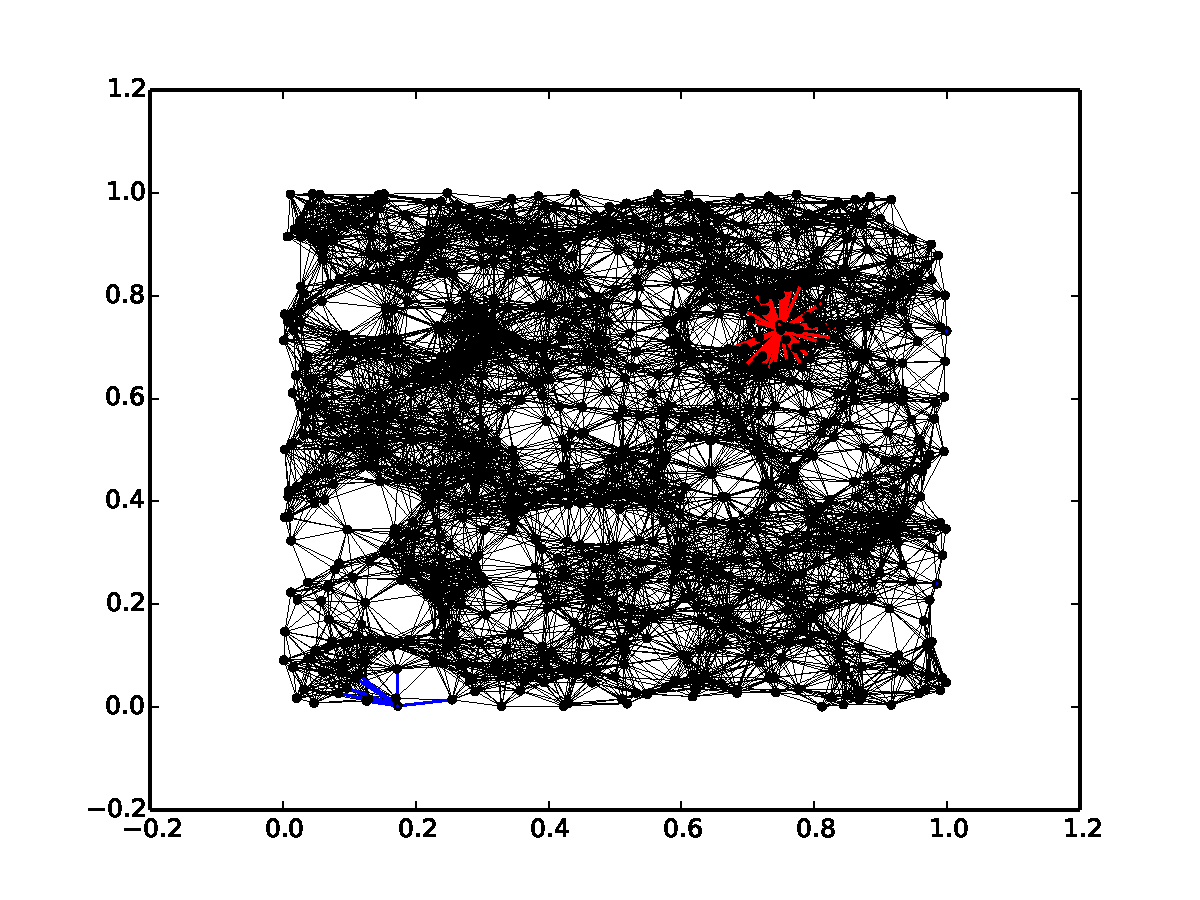
\includegraphics[width=0.9\linewidth]{figures/graph1.pdf}
	\caption{Graph}
\end{subfigure}%
\begin{subfigure}{0.5\textwidth}
	\centering
	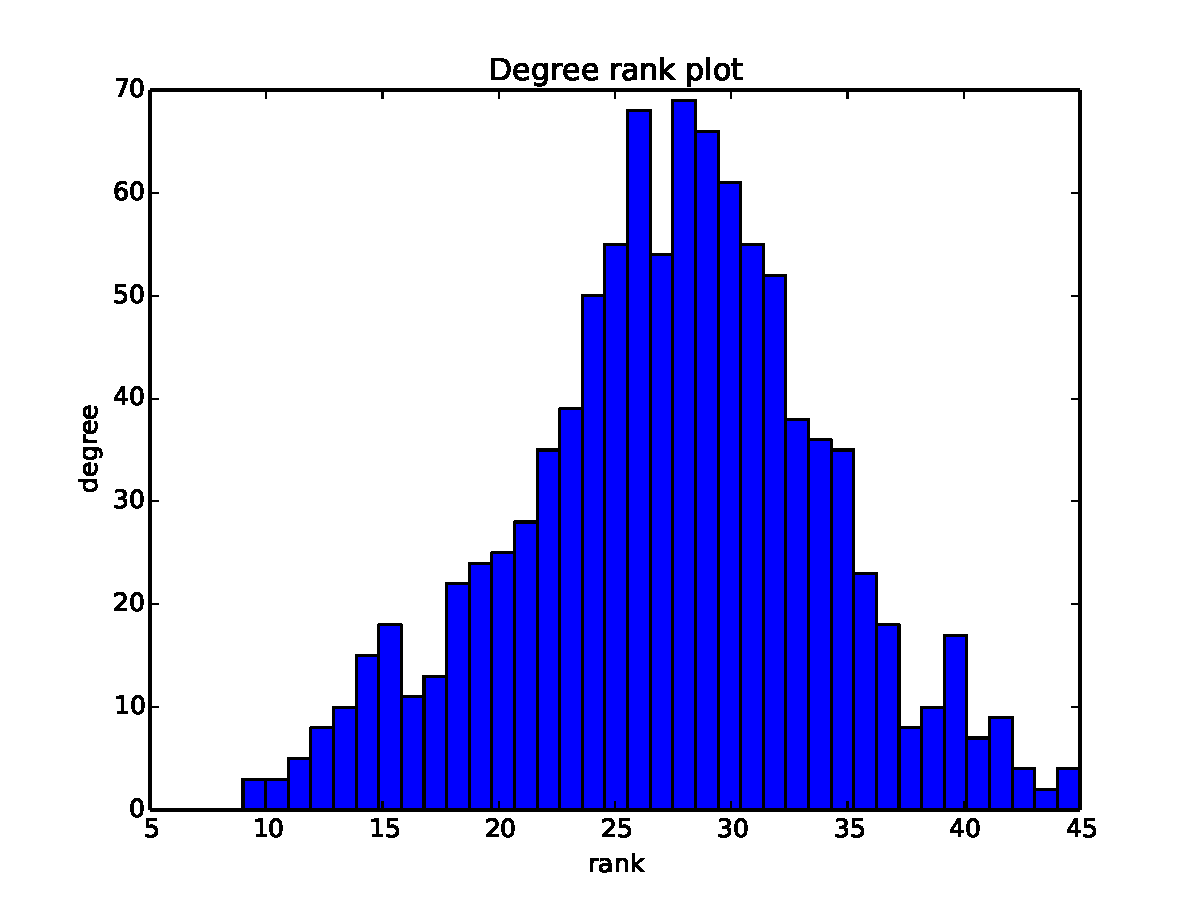
\includegraphics[width=0.9\linewidth]{figures/degrees1.pdf}
	\caption{Degree Histogram}
\end{subfigure}

\begin{subfigure}{0.5\textwidth}
	\centering
	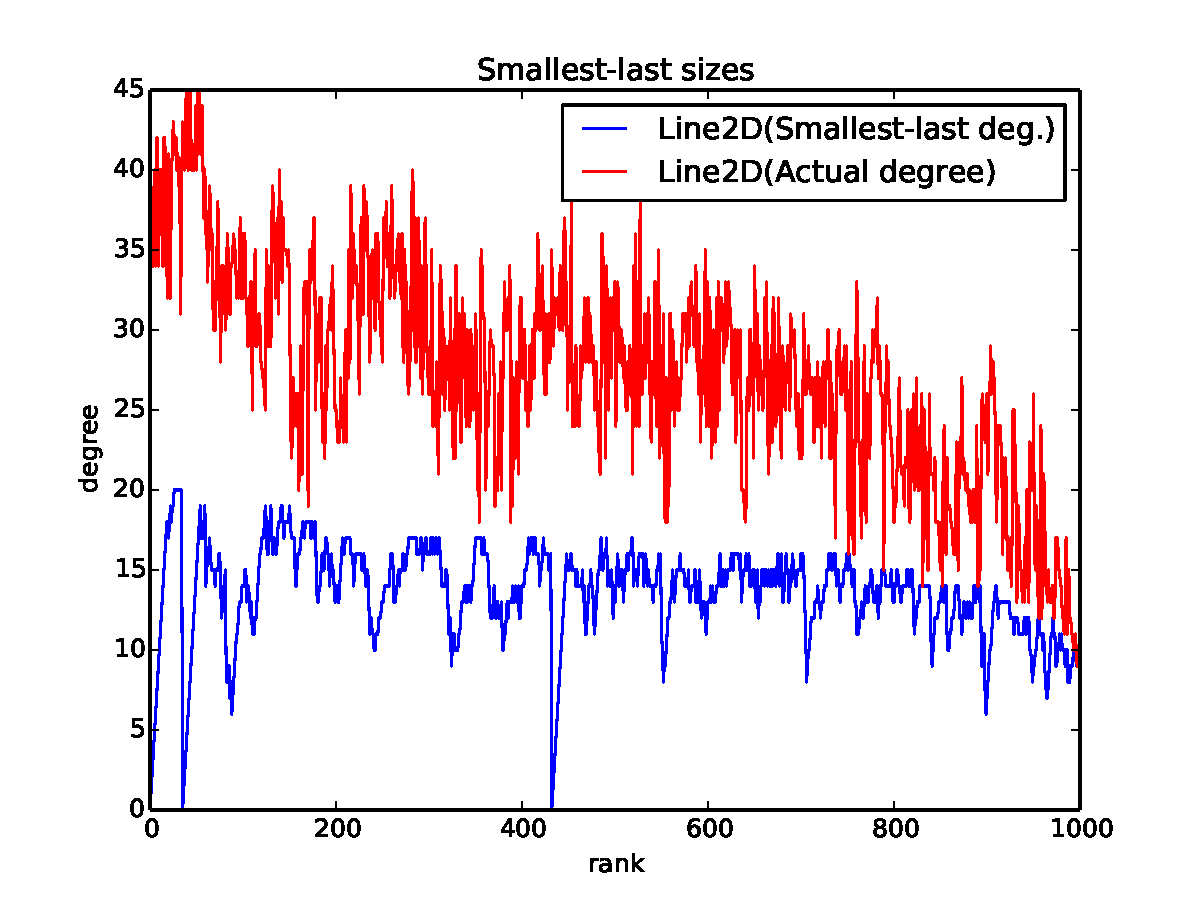
\includegraphics[width=0.9\linewidth]{figures/ordering1.pdf}
	\caption{Smallest--last degrees}
\end{subfigure}%
\begin{subfigure}{0.5\textwidth}
	\centering
	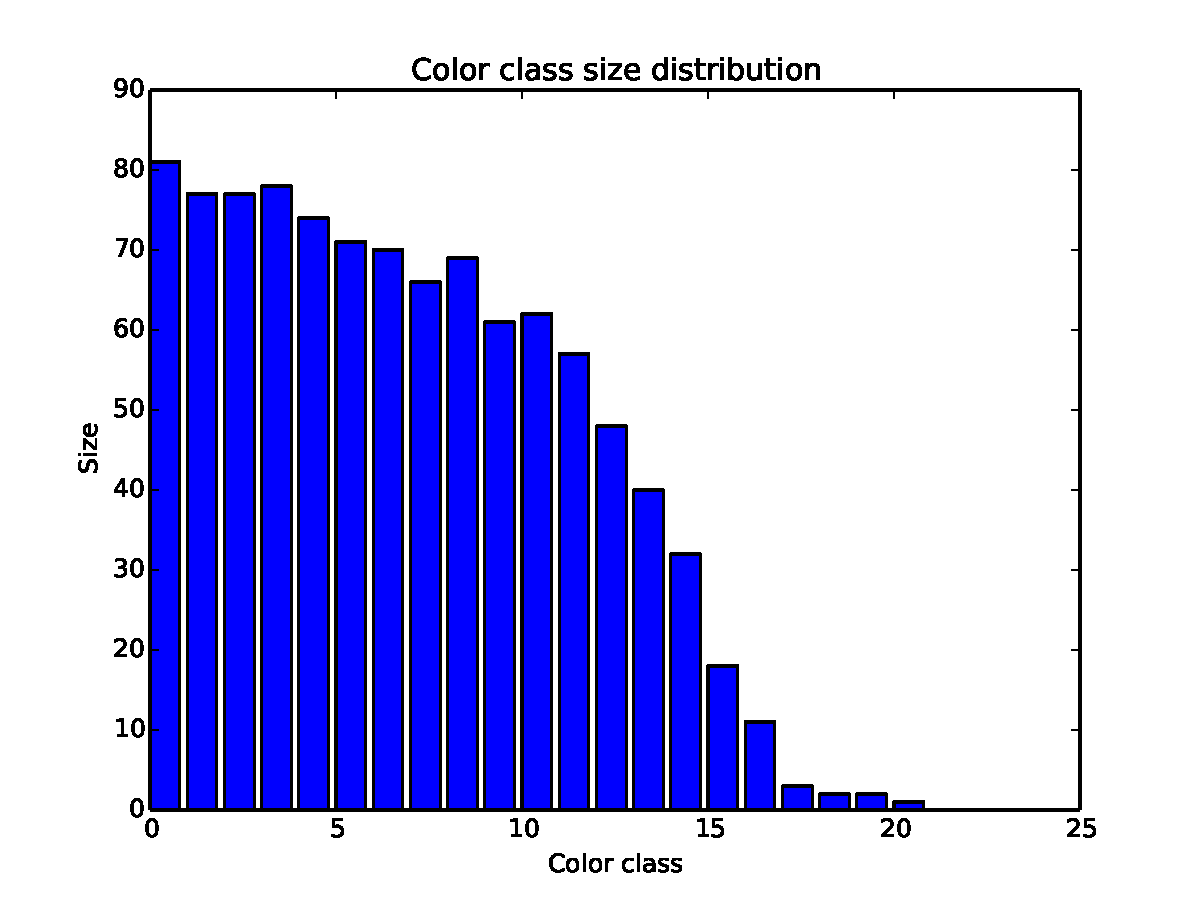
\includegraphics[width=0.9\linewidth]{figures/colors1.pdf}
	\caption{Color class sizes}
\end{subfigure}

\begin{subfigure}{0.5\textwidth}
	\centering
	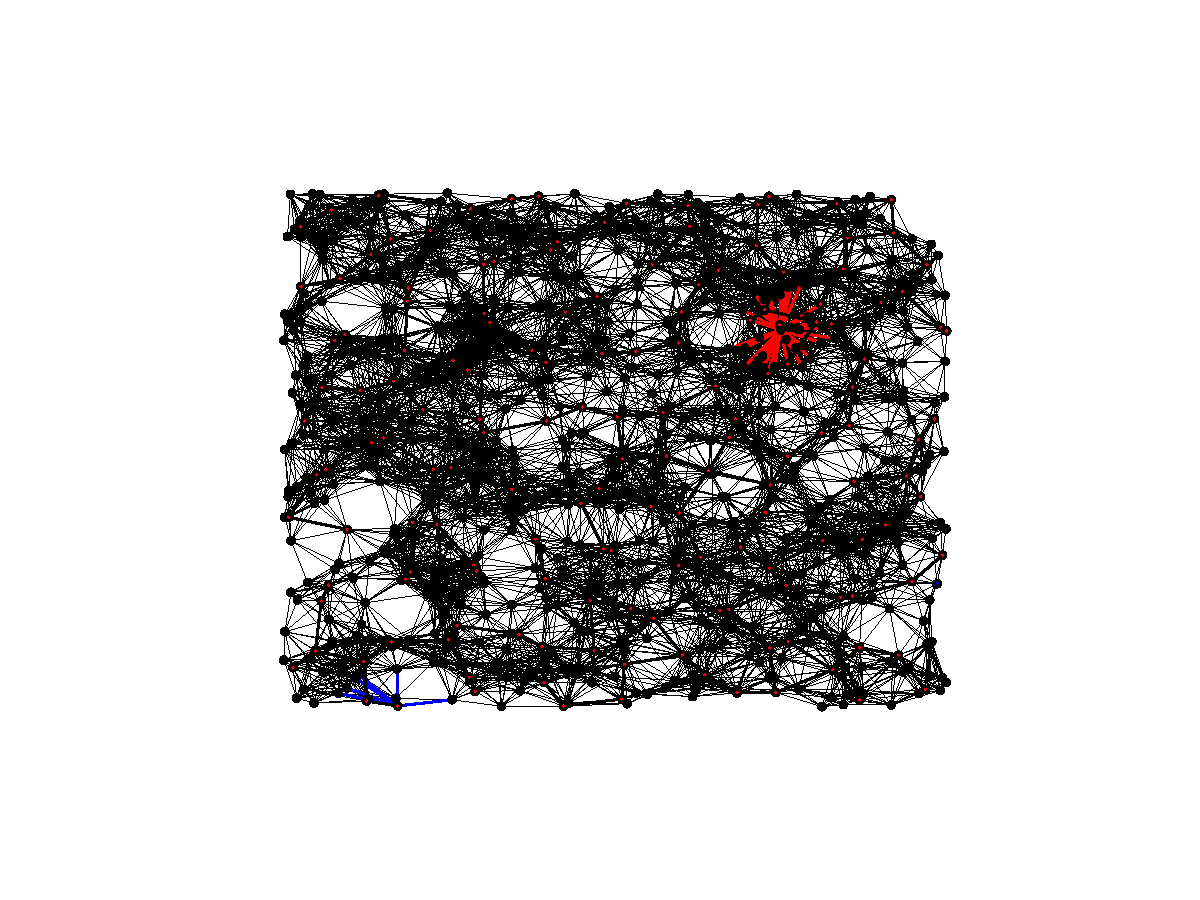
\includegraphics[width=0.9\linewidth]{figures/simplegraph1.pdf}
	\caption{Backbone 1}
\end{subfigure}%
\begin{subfigure}{0.5\textwidth}
	\centering
	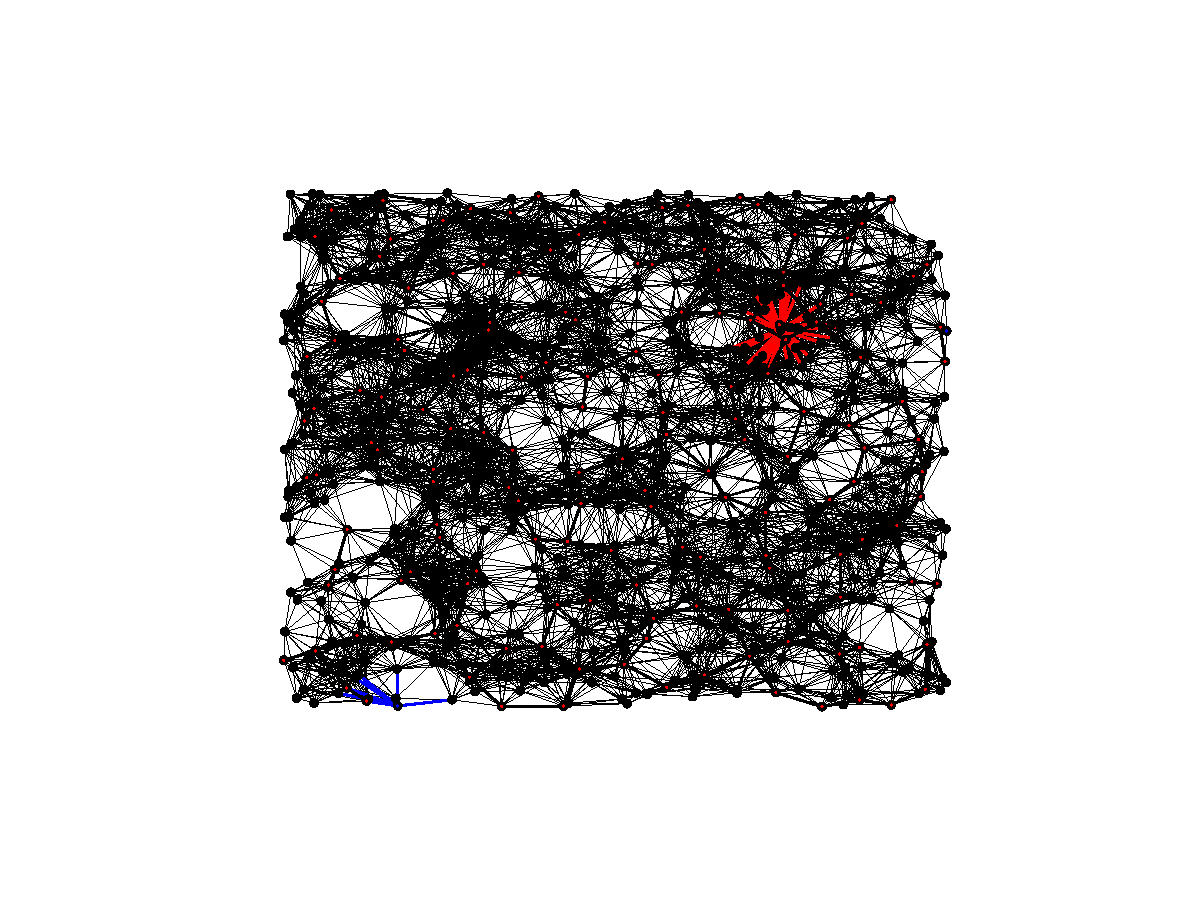
\includegraphics[width=0.9\linewidth]{figures/simplegraph11.pdf}
	\caption{Backbone 2}
\end{subfigure}
\end{figure}

\subsection{Square, $N=4000, \Delta_{avg}=40$}
\begin{figure}[!h]
\centering
\begin{subfigure}{0.5\textwidth}
	\centering
	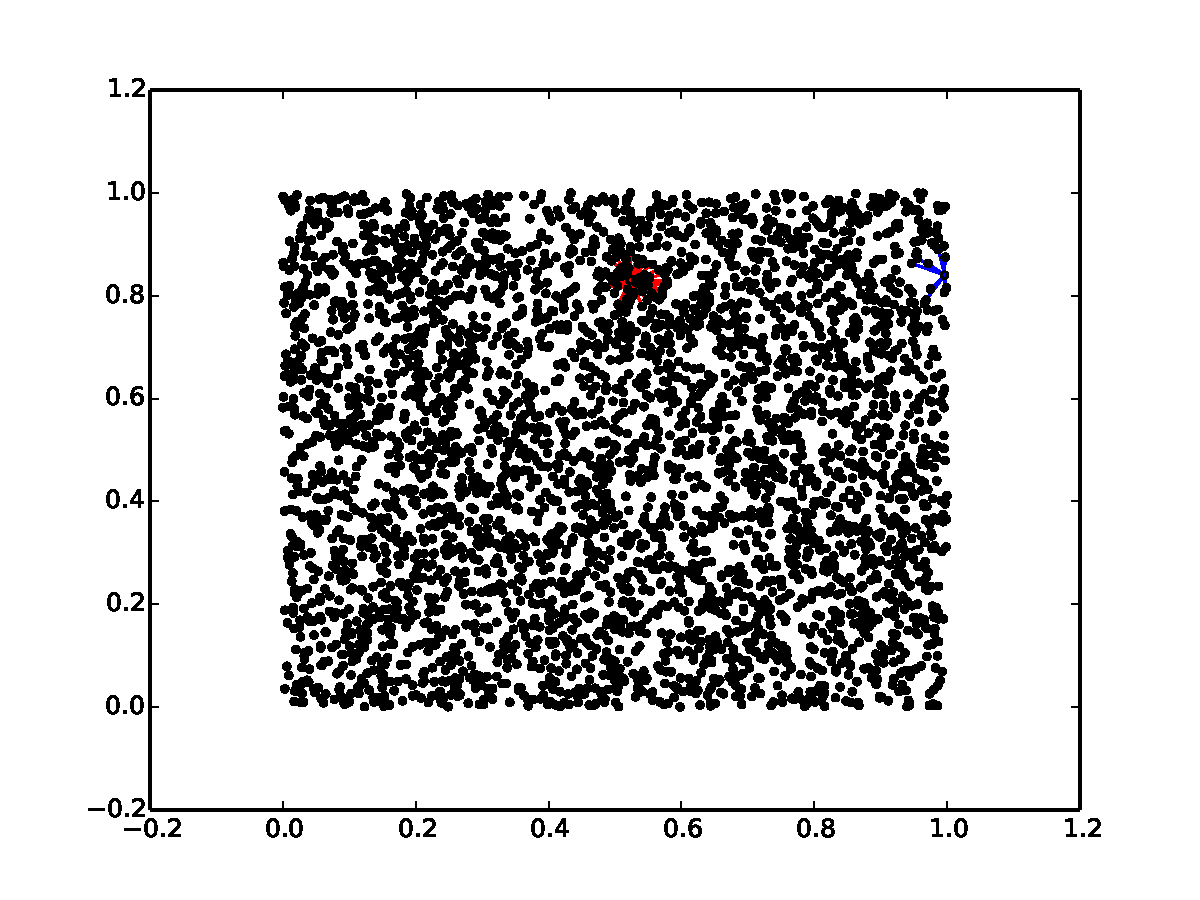
\includegraphics[width=0.9\linewidth]{figures/graph2.pdf}
	\caption{Graph}
\end{subfigure}%
\begin{subfigure}{0.5\textwidth}
	\centering
	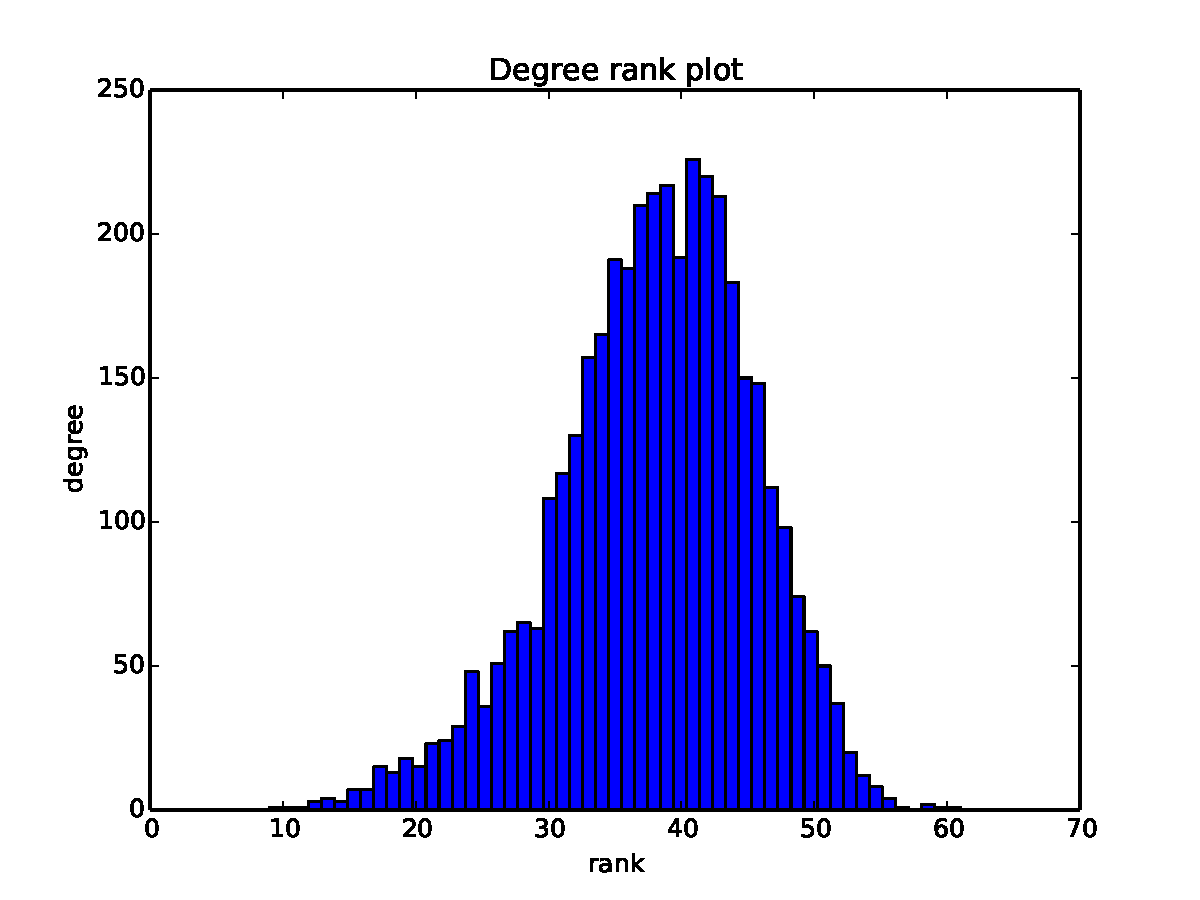
\includegraphics[width=0.9\linewidth]{figures/degrees2.pdf}
	\caption{Degree Histogram}
\end{subfigure}

\begin{subfigure}{0.5\textwidth}
	\centering
	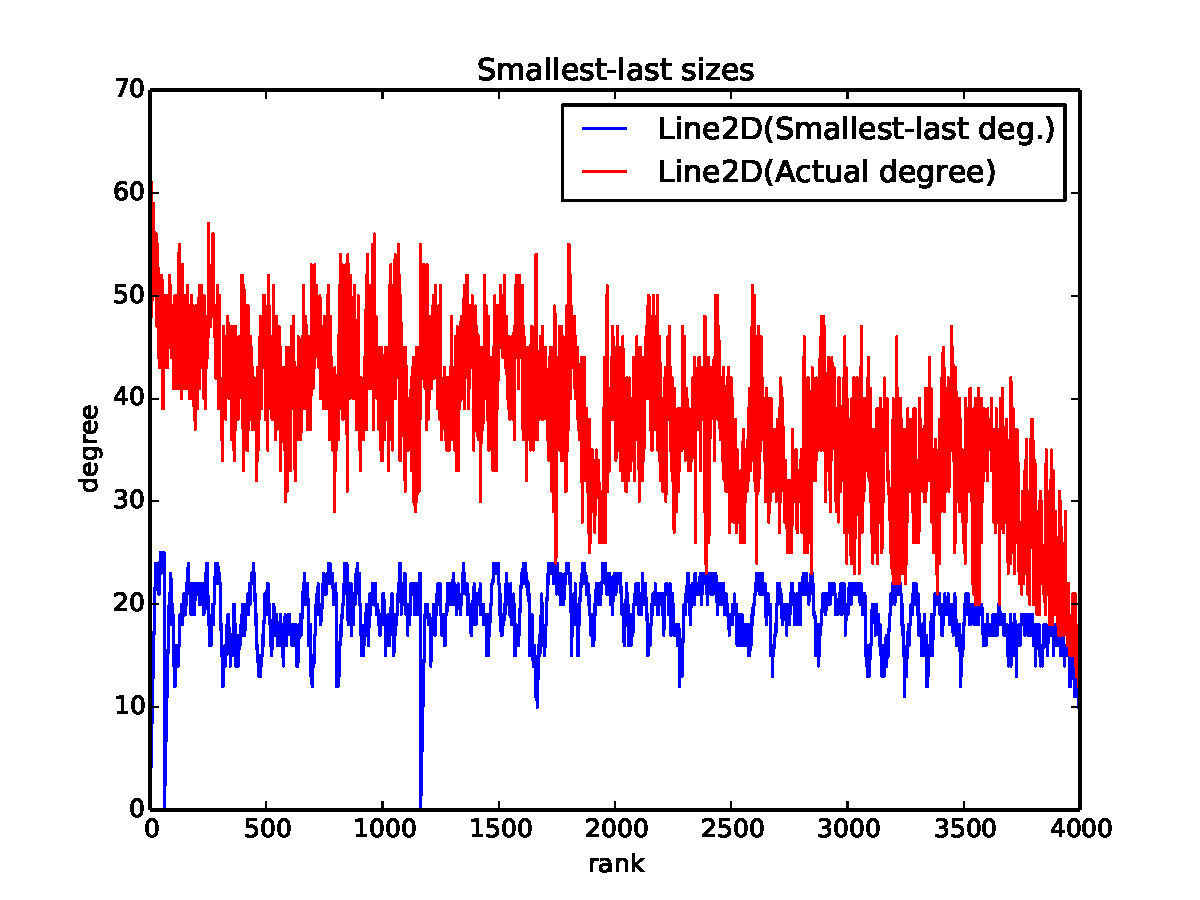
\includegraphics[width=0.9\linewidth]{figures/ordering2.pdf}
	\caption{Smallest--last degrees}
\end{subfigure}%
\begin{subfigure}{0.5\textwidth}
	\centering
	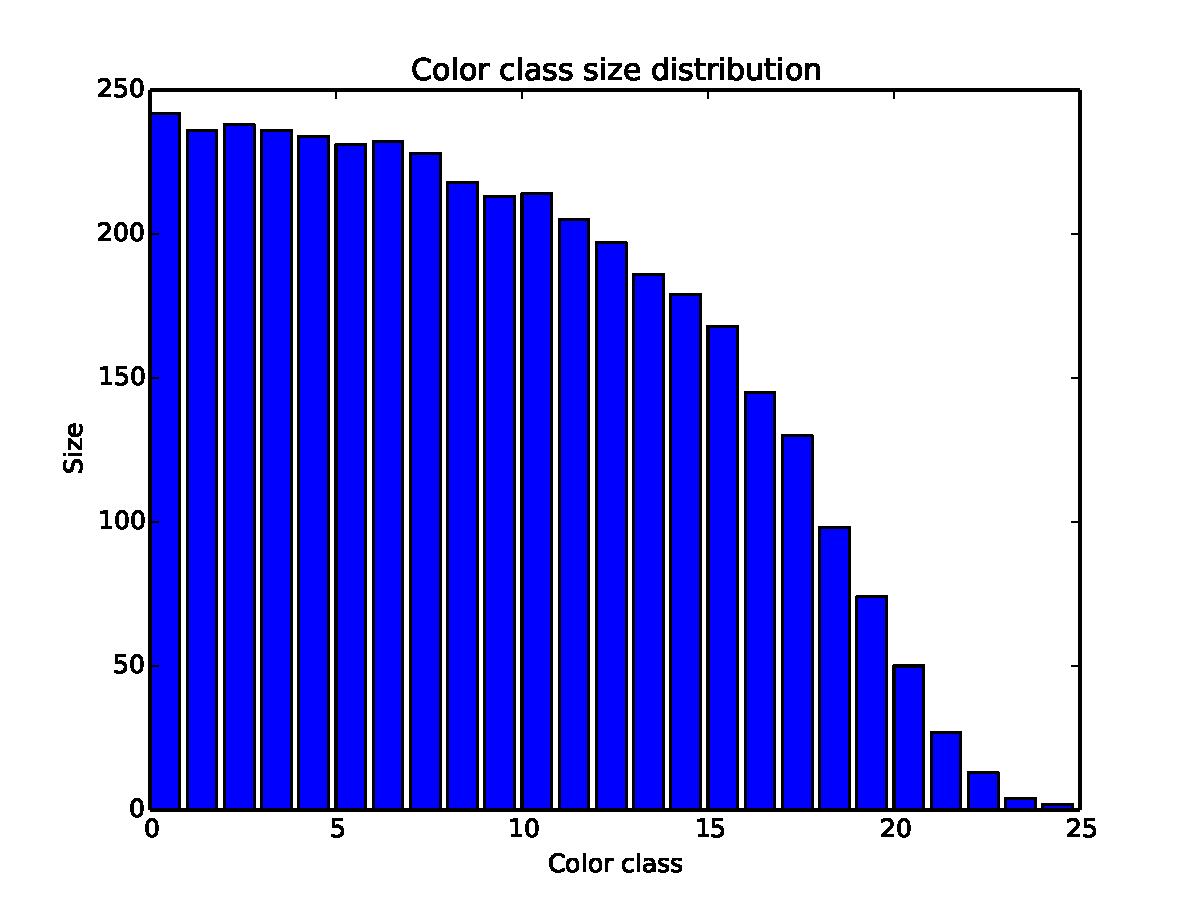
\includegraphics[width=0.9\linewidth]{figures/colors2.pdf}
	\caption{Color class sizes}
\end{subfigure}

\begin{subfigure}{0.5\textwidth}
	\centering
	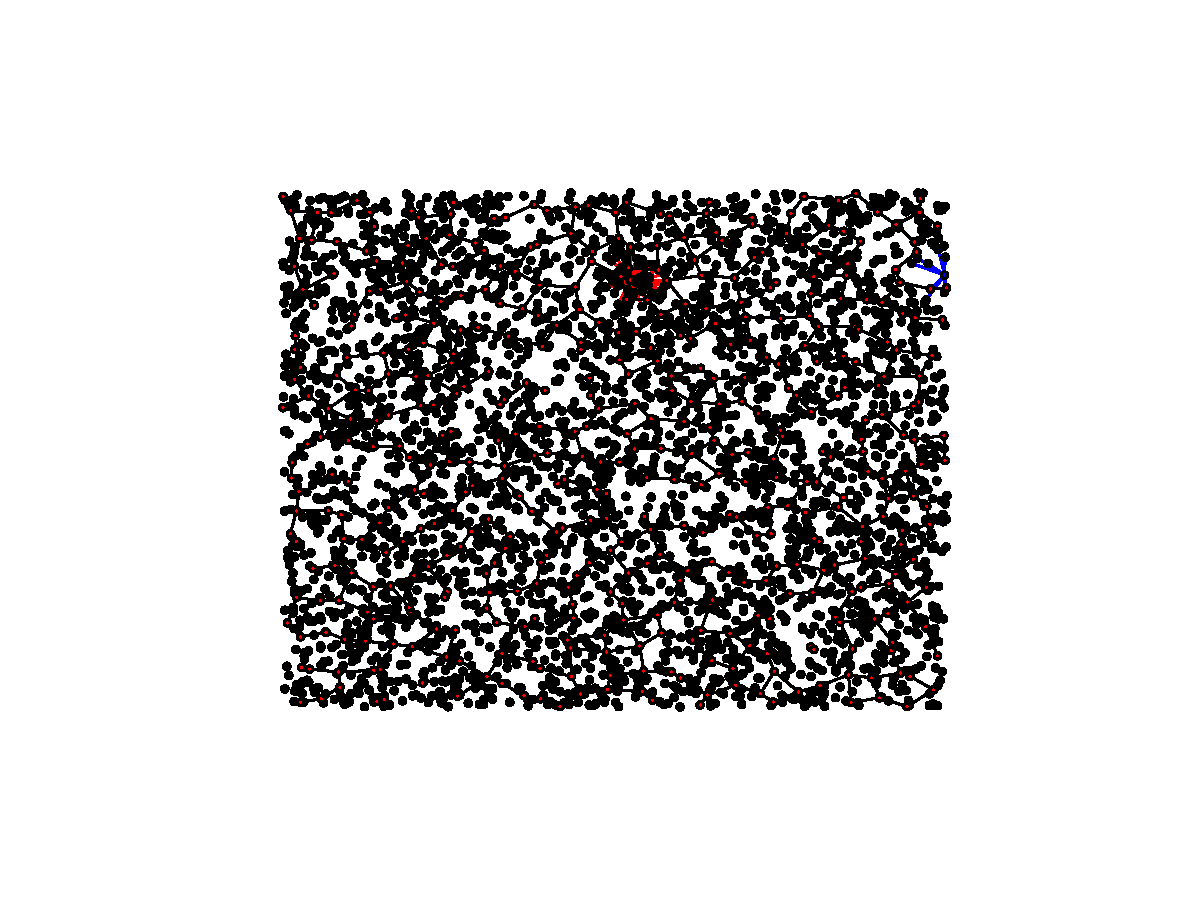
\includegraphics[width=0.9\linewidth]{figures/simplegraph2.pdf}
	\caption{Backbone 1}
\end{subfigure}%
\begin{subfigure}{0.5\textwidth}
	\centering
	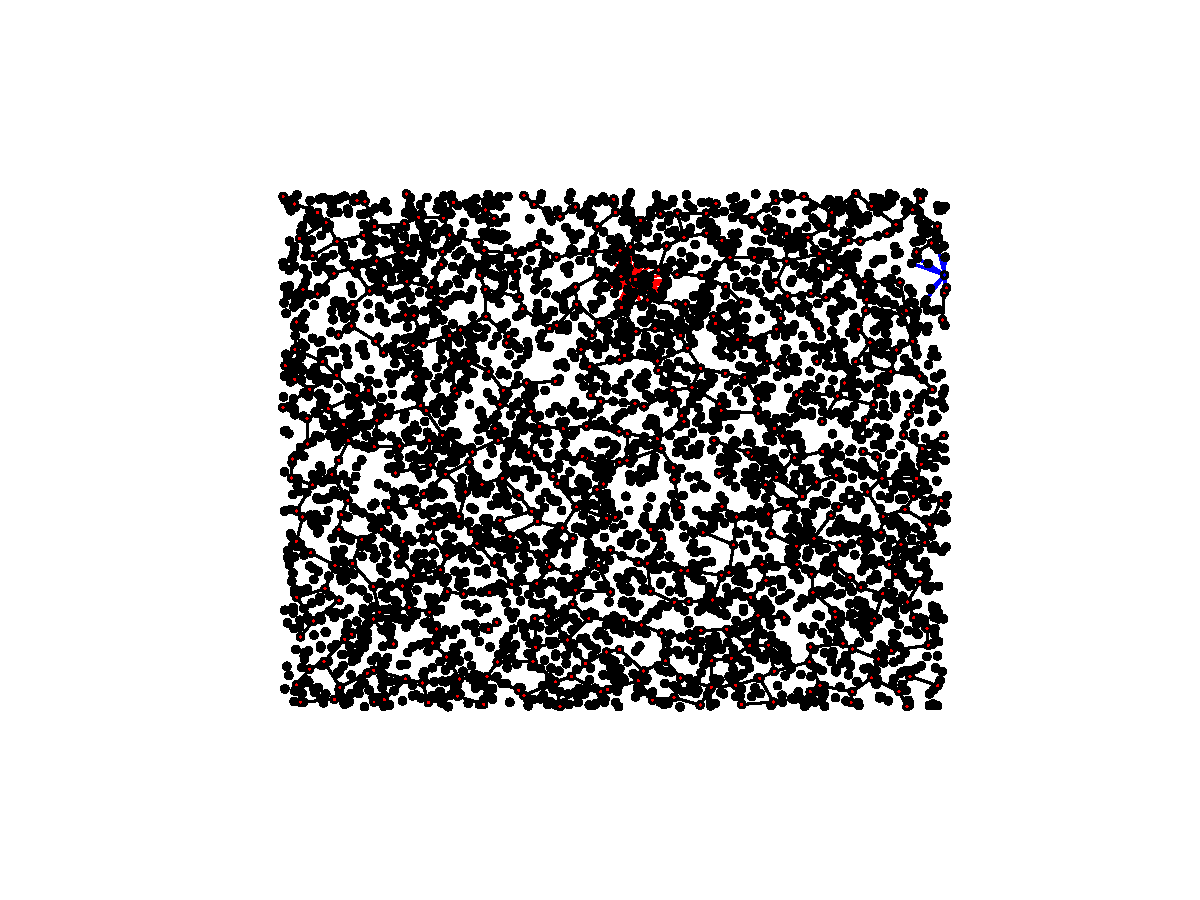
\includegraphics[width=0.9\linewidth]{figures/simplegraph21.pdf}
	\caption{Backbone 2}
\end{subfigure}
\end{figure}

\subsection{Square, $N=4000, \Delta_{avg}=60$}
\begin{figure}[!h]
\centering
\begin{subfigure}{0.5\textwidth}
	\centering
	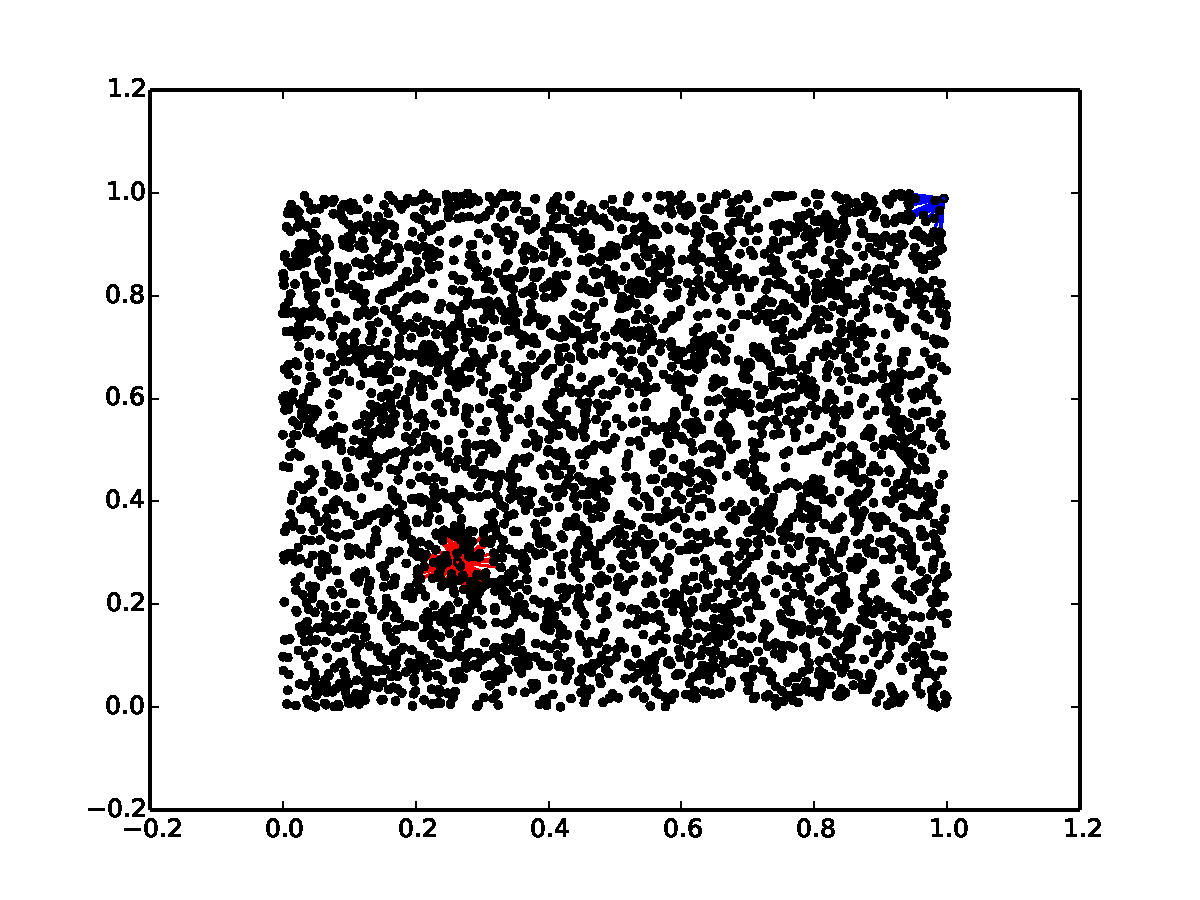
\includegraphics[width=0.9\linewidth]{figures/graph3.pdf}
	\caption{Graph}
\end{subfigure}%
\begin{subfigure}{0.5\textwidth}
	\centering
	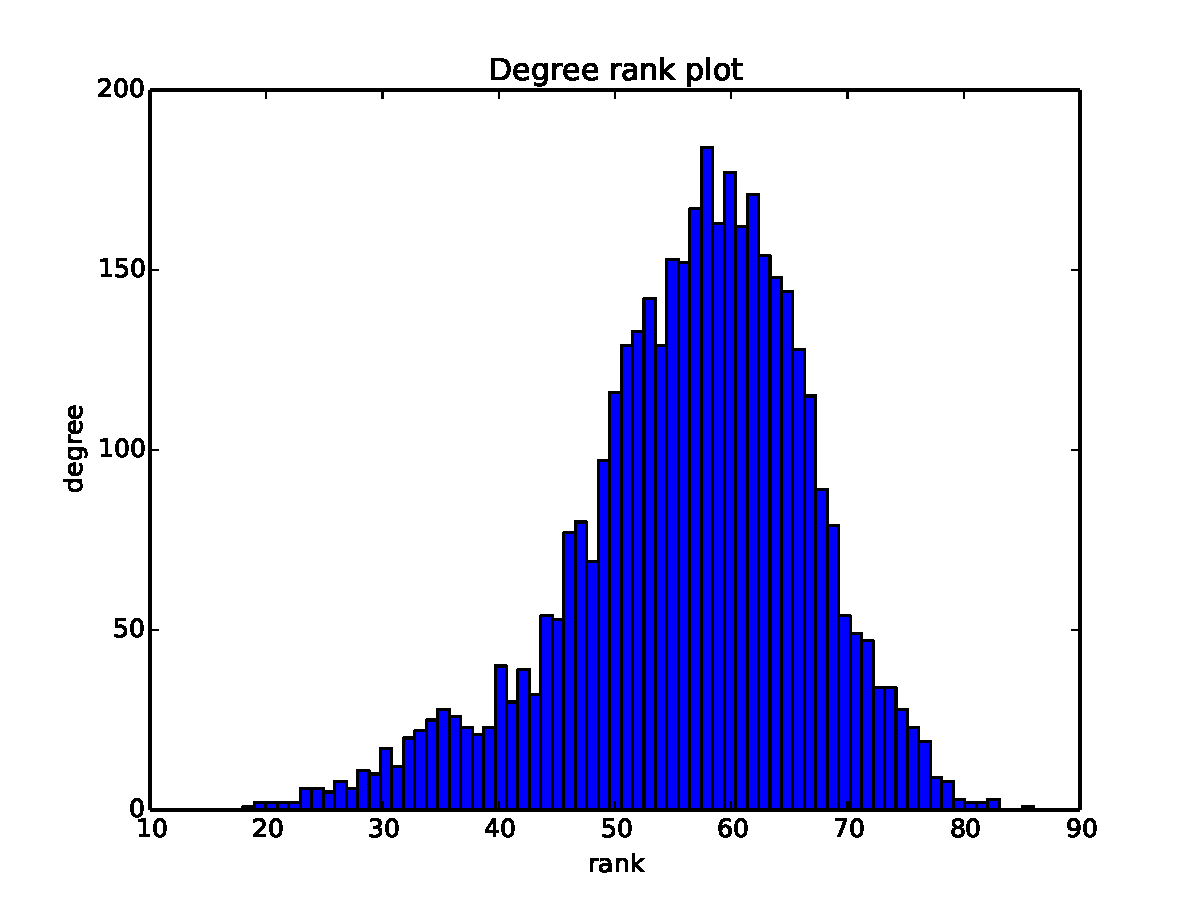
\includegraphics[width=0.9\linewidth]{figures/degrees3.pdf}
	\caption{Degree Histogram}
\end{subfigure}

\begin{subfigure}{0.5\textwidth}
	\centering
	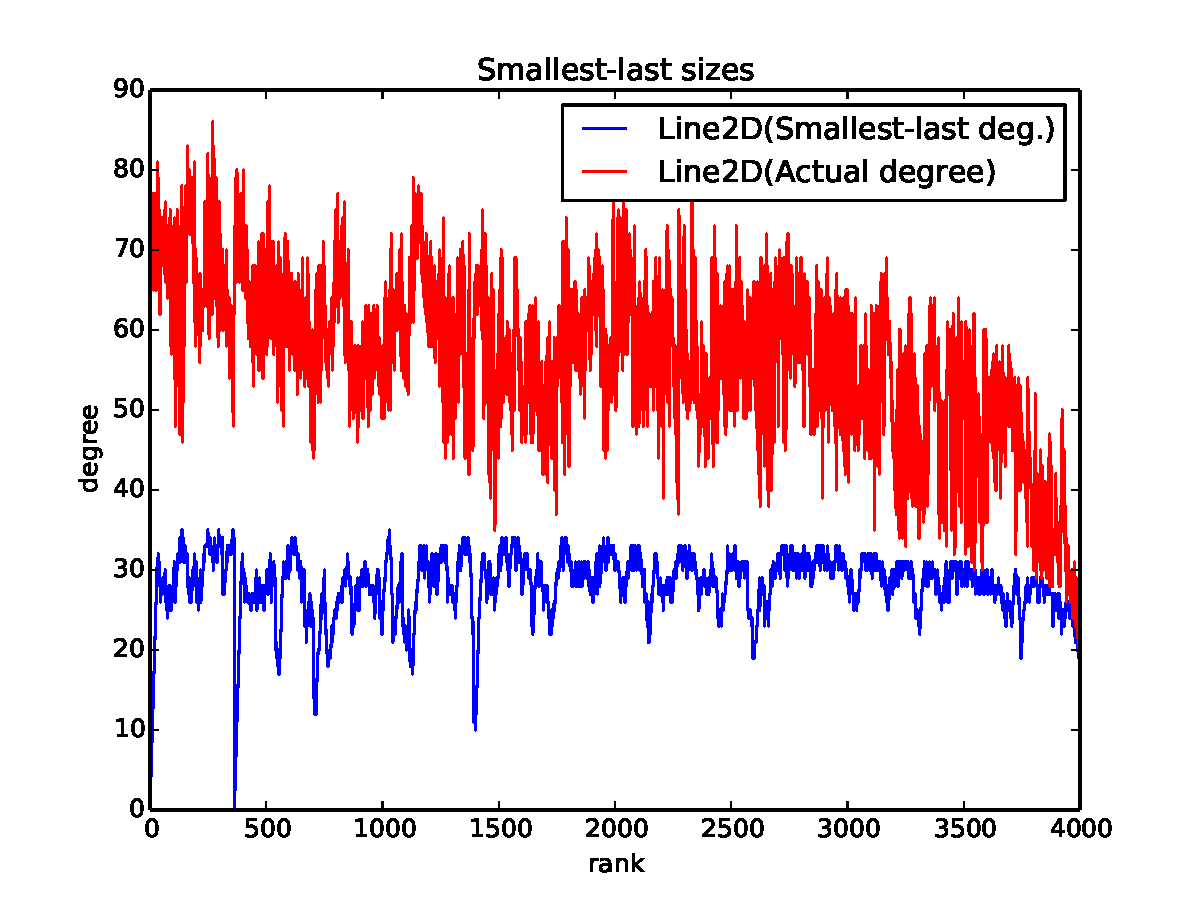
\includegraphics[width=0.9\linewidth]{figures/ordering3.pdf}
	\caption{Smallest--last degrees}
\end{subfigure}%
\begin{subfigure}{0.5\textwidth}
	\centering
	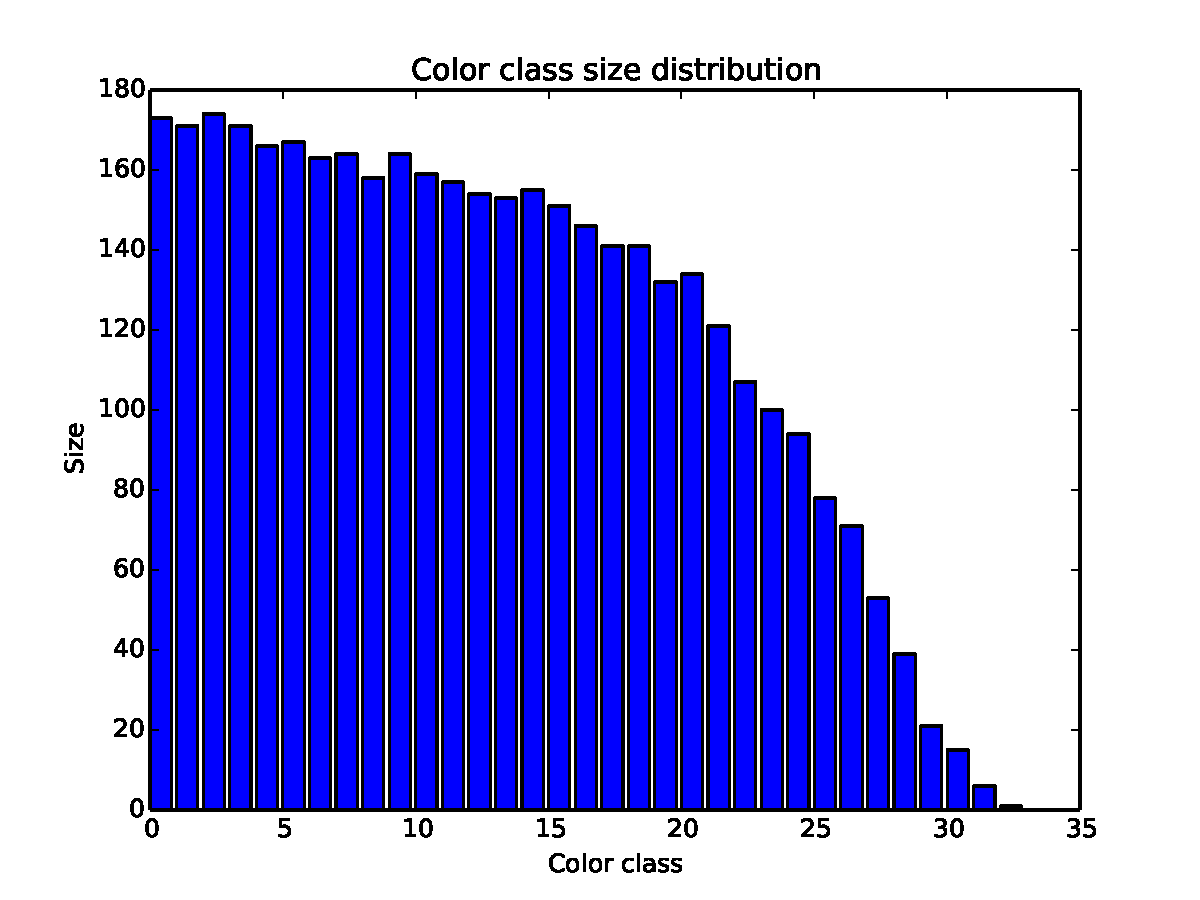
\includegraphics[width=0.9\linewidth]{figures/colors3.pdf}
	\caption{Color class sizes}
\end{subfigure}

\begin{subfigure}{0.5\textwidth}
	\centering
	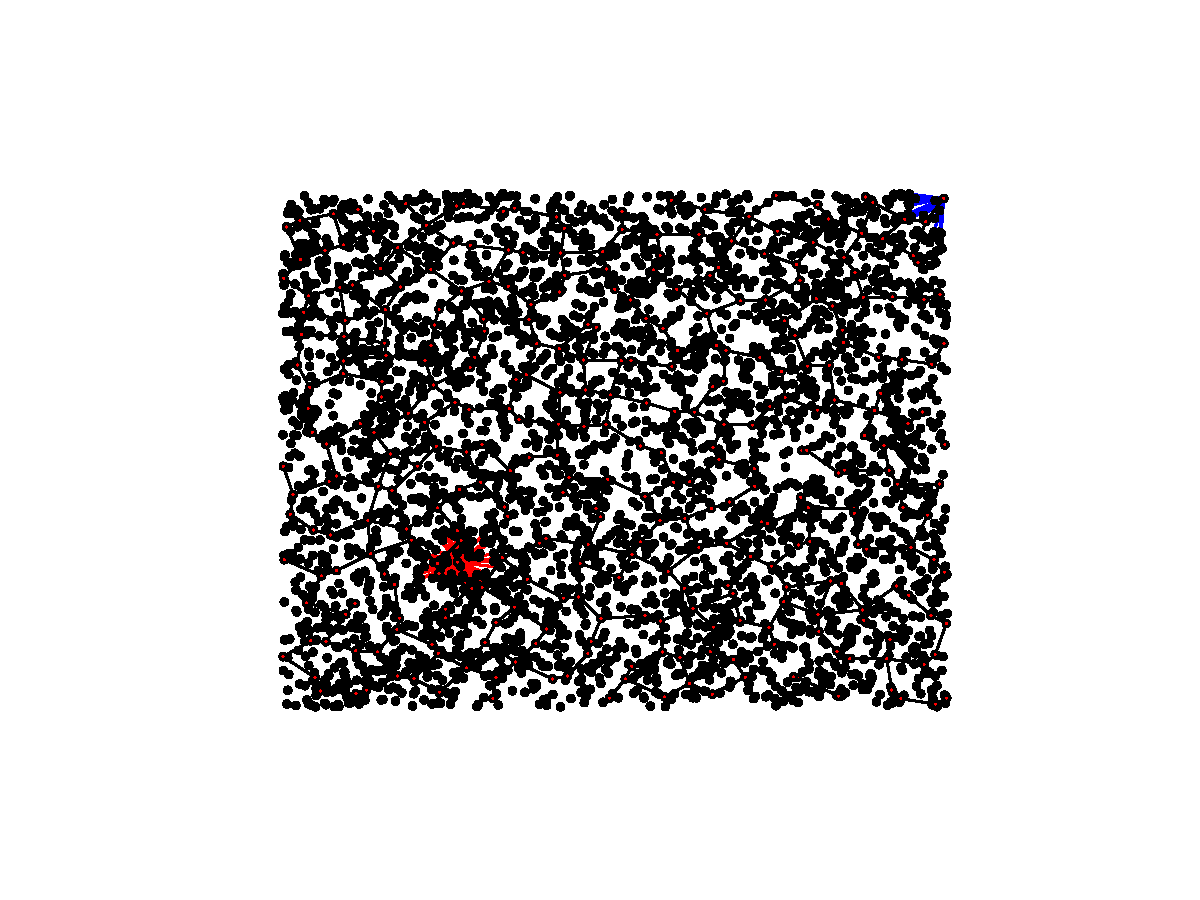
\includegraphics[width=0.9\linewidth]{figures/simplegraph3.pdf}
	\caption{Backbone 1}
\end{subfigure}%
\begin{subfigure}{0.5\textwidth}
	\centering
	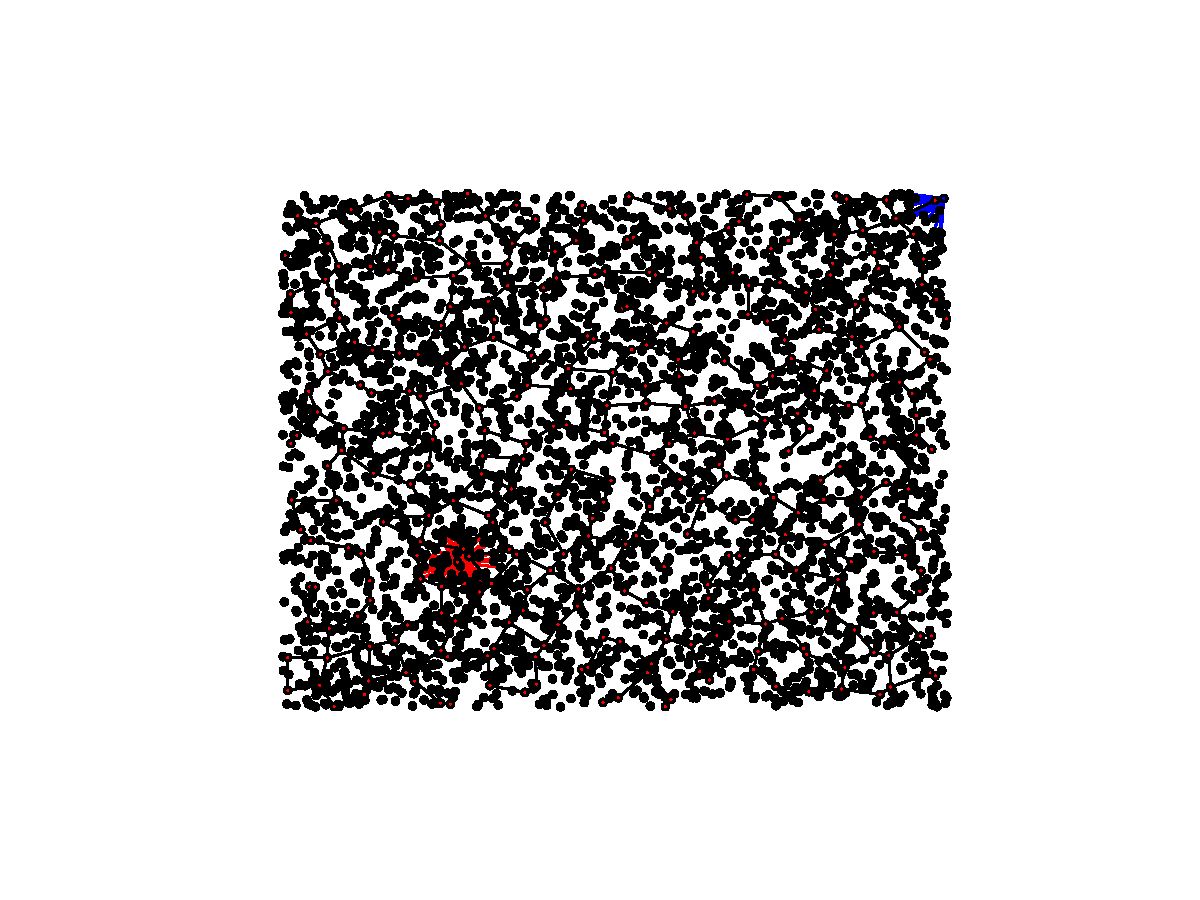
\includegraphics[width=0.9\linewidth]{figures/simplegraph31.pdf}
	\caption{Backbone 2}
\end{subfigure}
\end{figure}

\subsection{Square, $N=16000, \Delta_{avg}=60$}
\begin{figure}[!h]
\centering
\begin{subfigure}{0.5\textwidth}
	\centering
	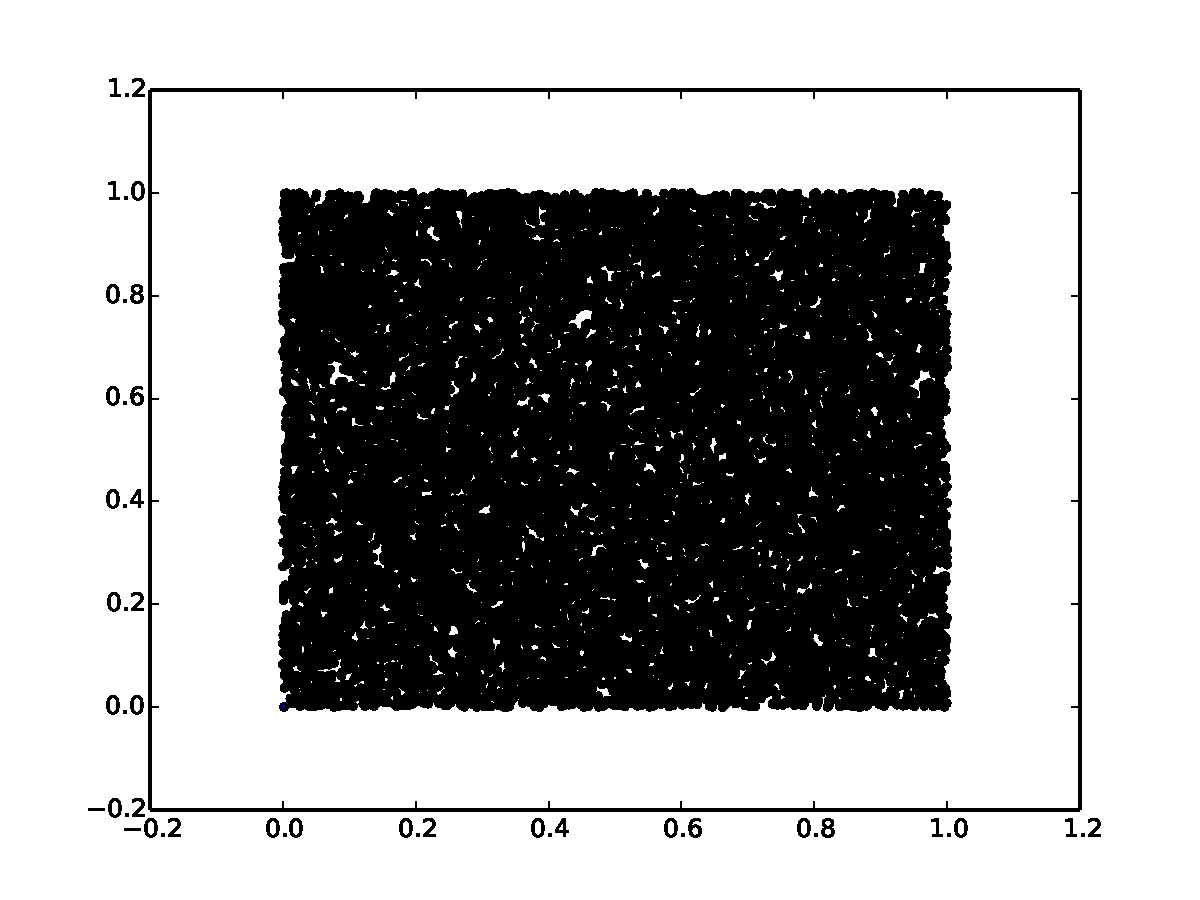
\includegraphics[width=0.9\linewidth]{figures/graph4.pdf}
	\caption{Graph}
\end{subfigure}%
\begin{subfigure}{0.5\textwidth}
	\centering
	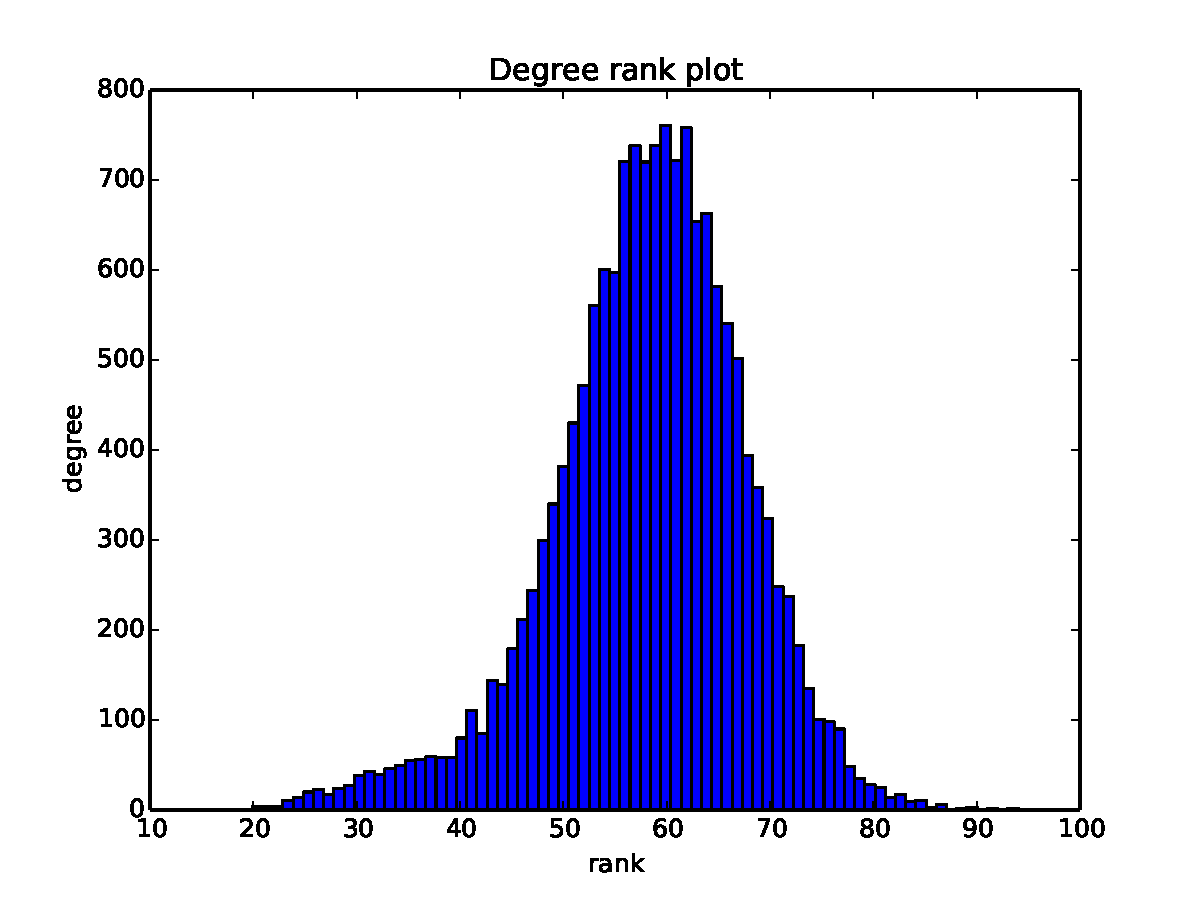
\includegraphics[width=0.9\linewidth]{figures/degrees4.pdf}
	\caption{Degree Histogram}
\end{subfigure}

\begin{subfigure}{0.5\textwidth}
	\centering
	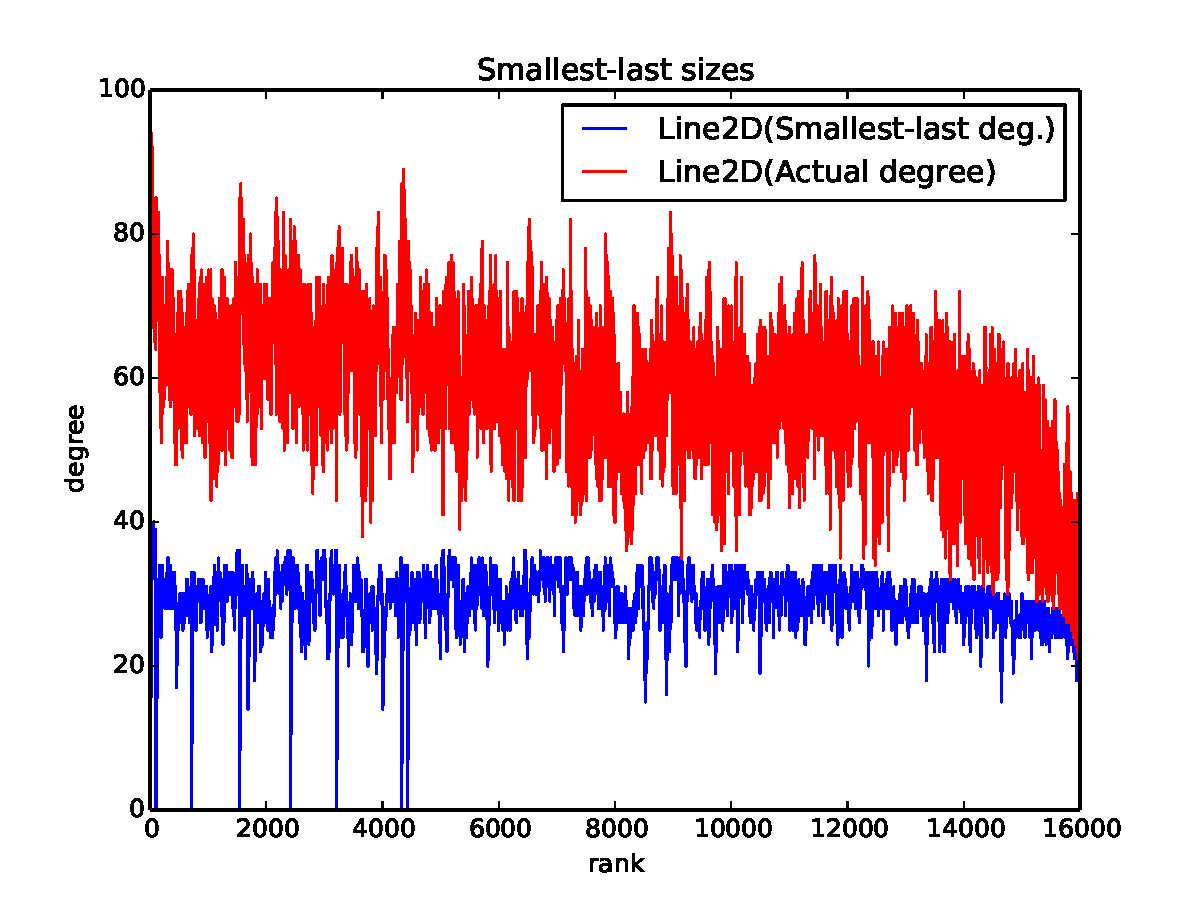
\includegraphics[width=0.9\linewidth]{figures/ordering4.pdf}
	\caption{Smallest--last degrees}
\end{subfigure}%
\begin{subfigure}{0.5\textwidth}
	\centering
	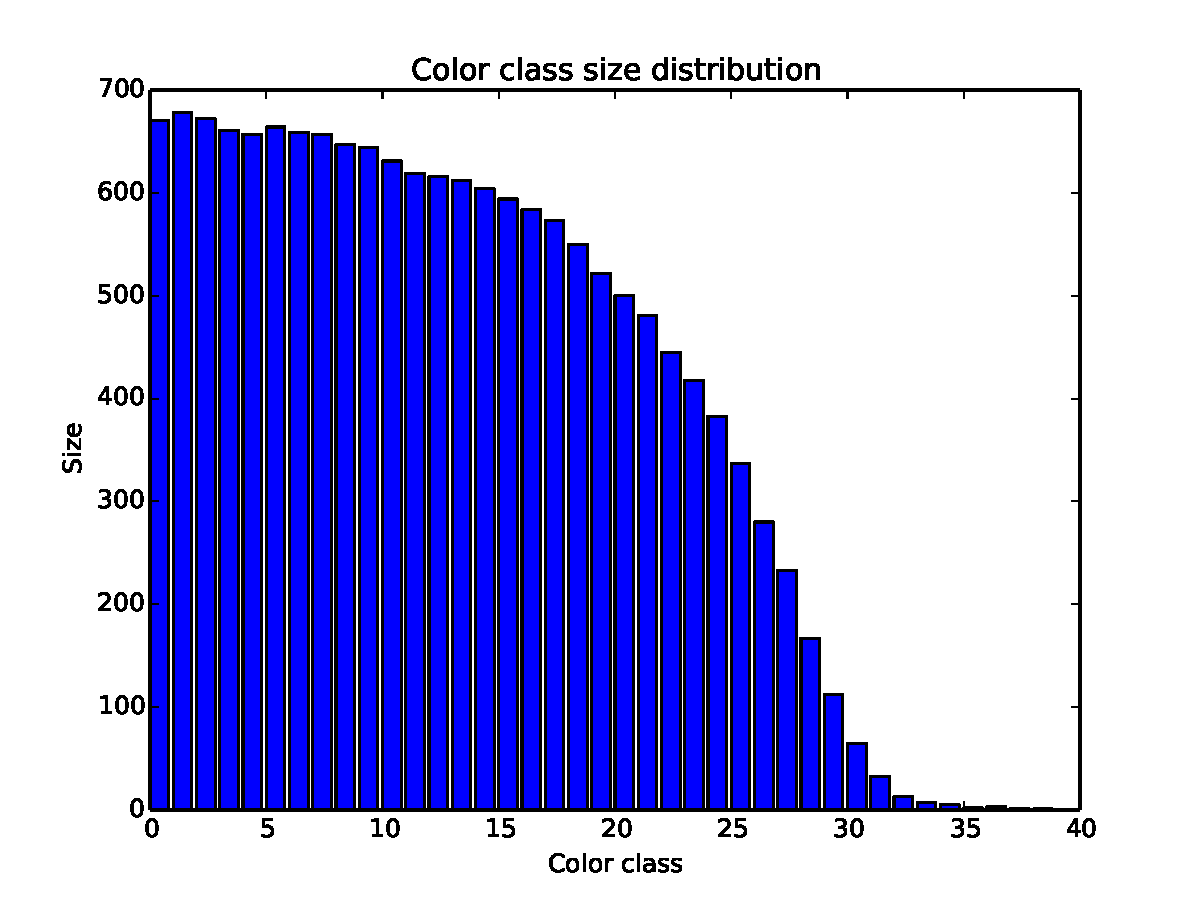
\includegraphics[width=0.9\linewidth]{figures/colors4.pdf}
	\caption{Color class sizes}
\end{subfigure}

\begin{subfigure}{0.5\textwidth}
	\centering
	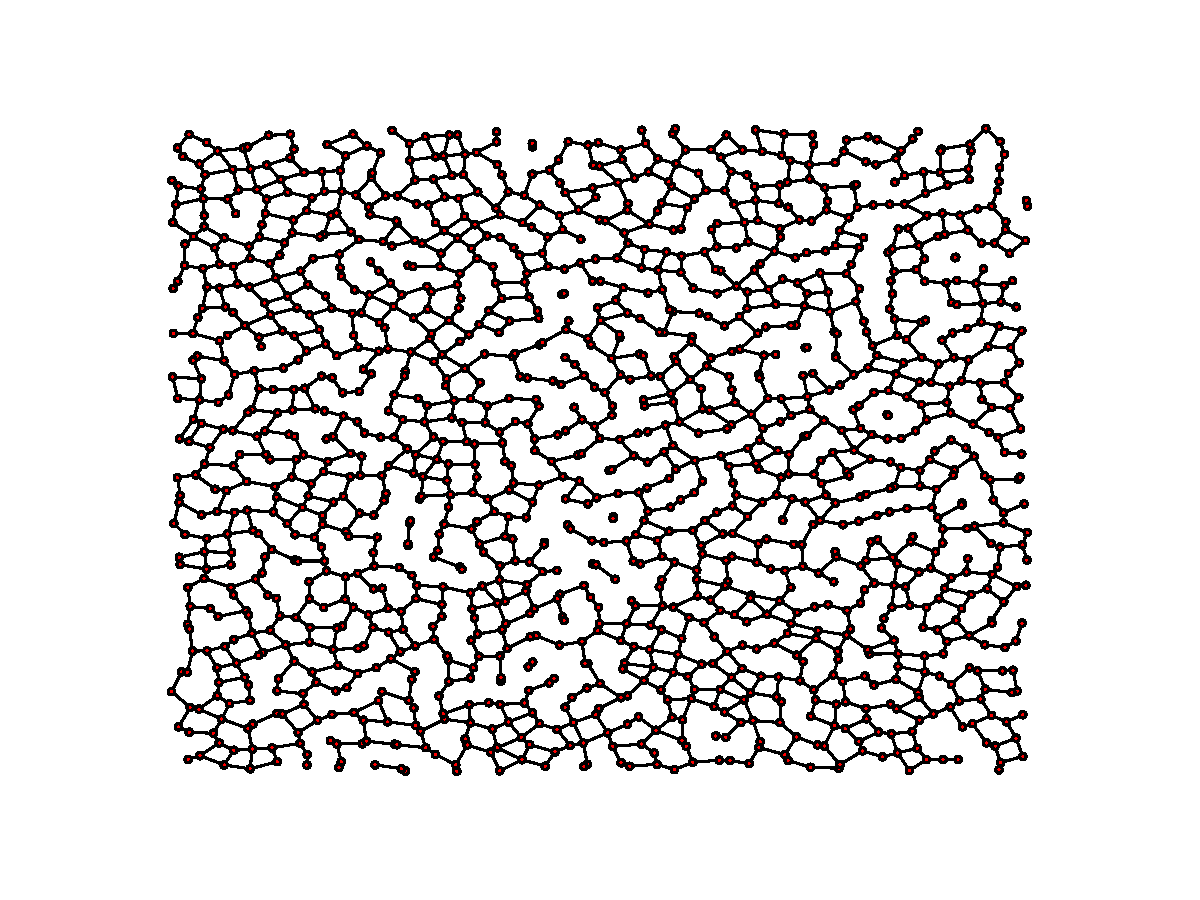
\includegraphics[width=0.9\linewidth]{figures/simplegraph4.pdf}
	\caption{Backbone 1}
\end{subfigure}%
\begin{subfigure}{0.5\textwidth}
	\centering
	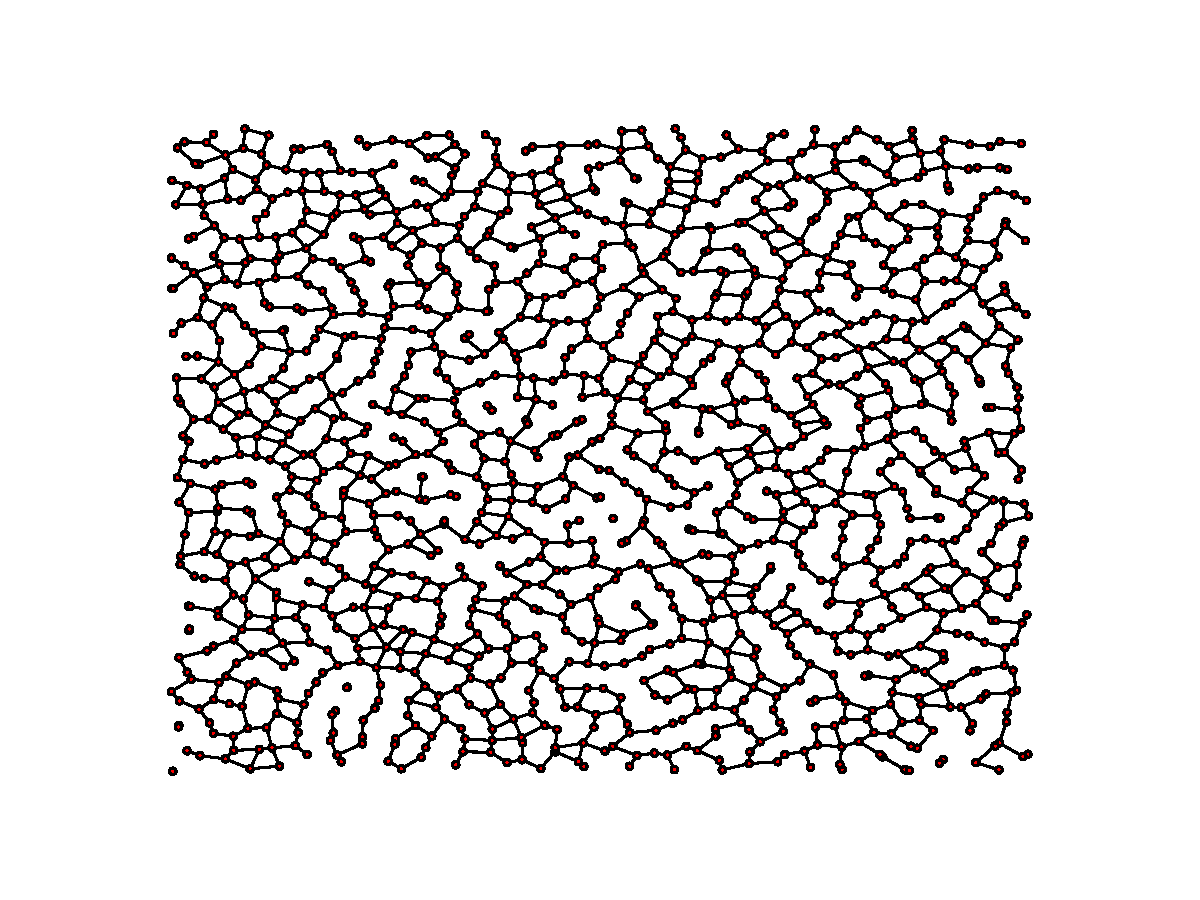
\includegraphics[width=0.9\linewidth]{figures/simplegraph41.pdf}
	\caption{Backbone 2}
\end{subfigure}
\end{figure}

\subsection{Square, $N=64000, \Delta_{avg}=60$}
\begin{figure}[!h]
\centering
\begin{subfigure}{0.5\textwidth}
	\centering
	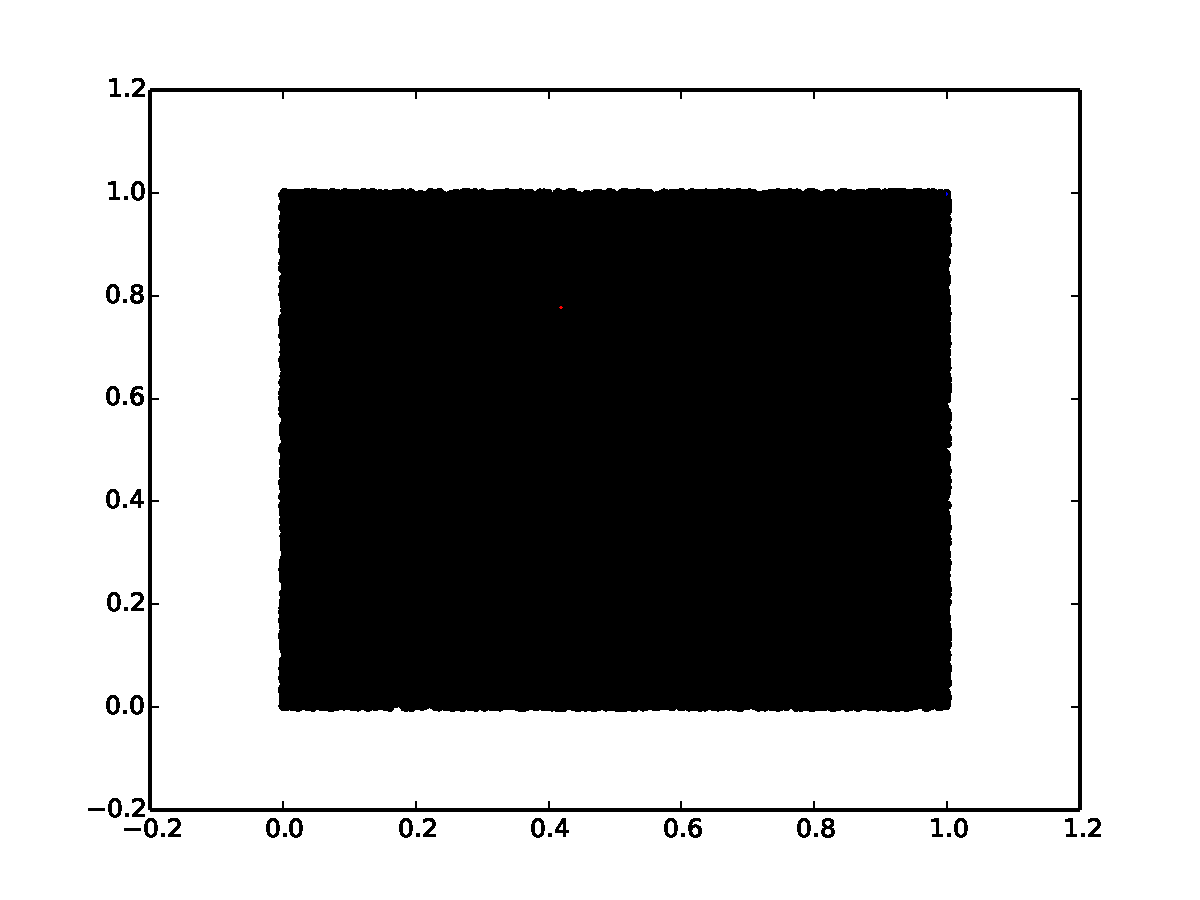
\includegraphics[width=0.9\linewidth]{figures/graph5.pdf}
	\caption{Graph}
\end{subfigure}%
\begin{subfigure}{0.5\textwidth}
	\centering
	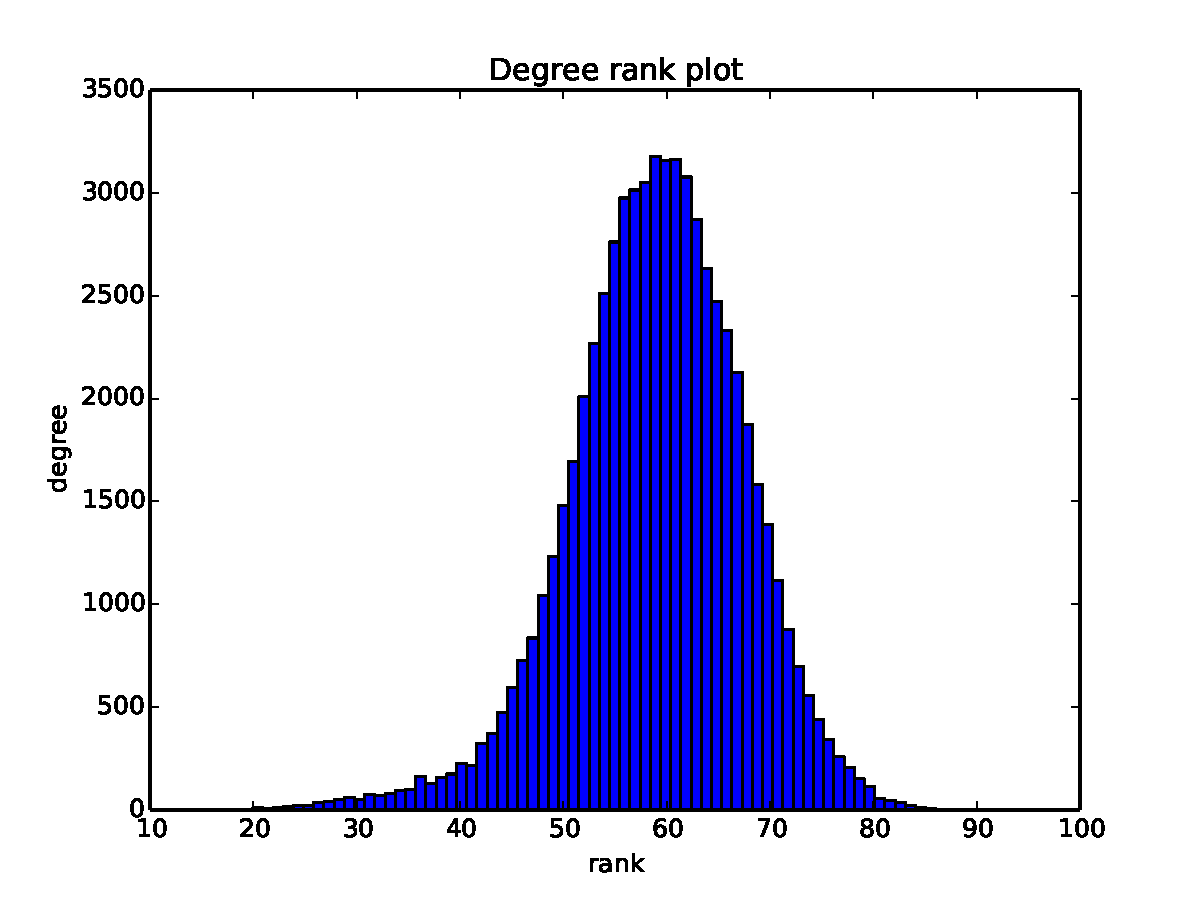
\includegraphics[width=0.9\linewidth]{figures/degrees5.pdf}
	\caption{Degree Histogram}
\end{subfigure}

\begin{subfigure}{0.5\textwidth}
	\centering
	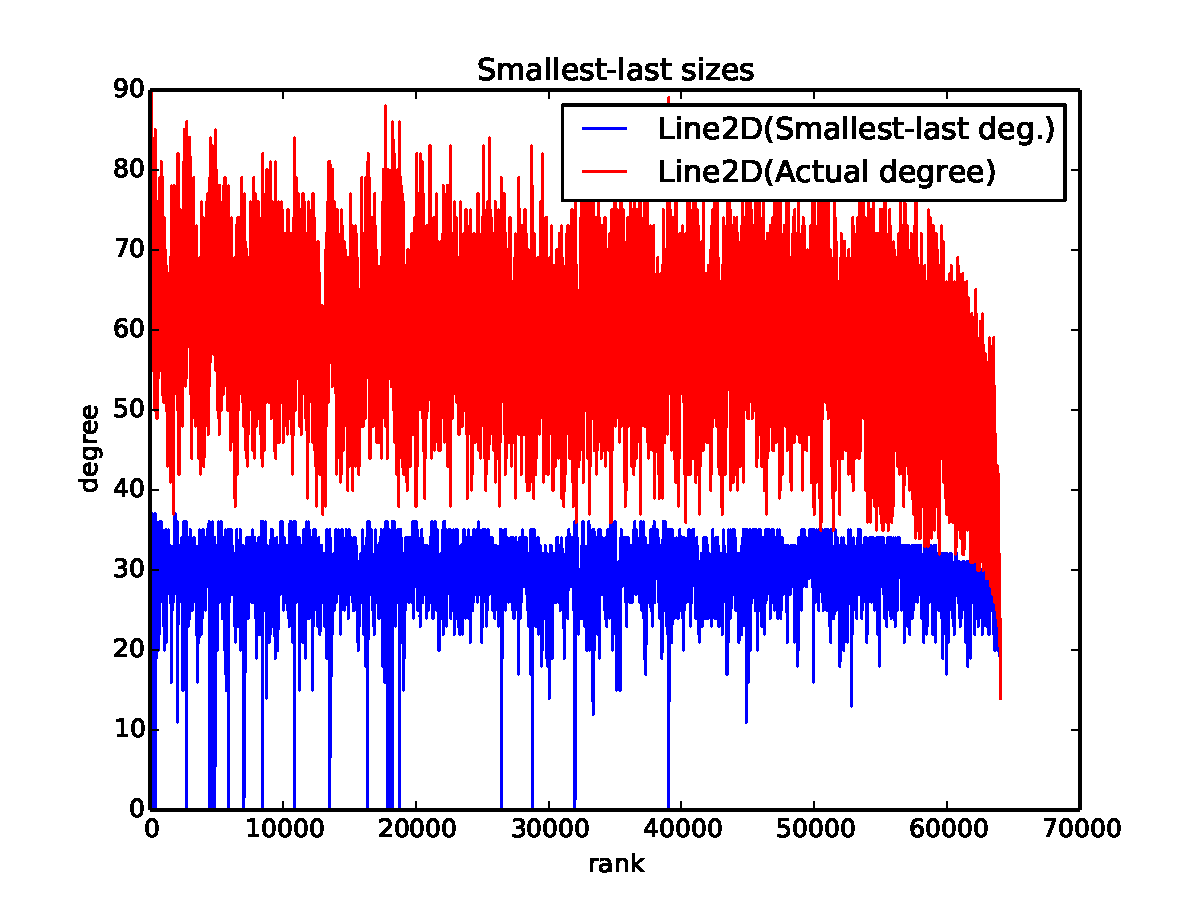
\includegraphics[width=0.9\linewidth]{figures/ordering5.pdf}
	\caption{Smallest--last degrees}
\end{subfigure}%
\begin{subfigure}{0.5\textwidth}
	\centering
	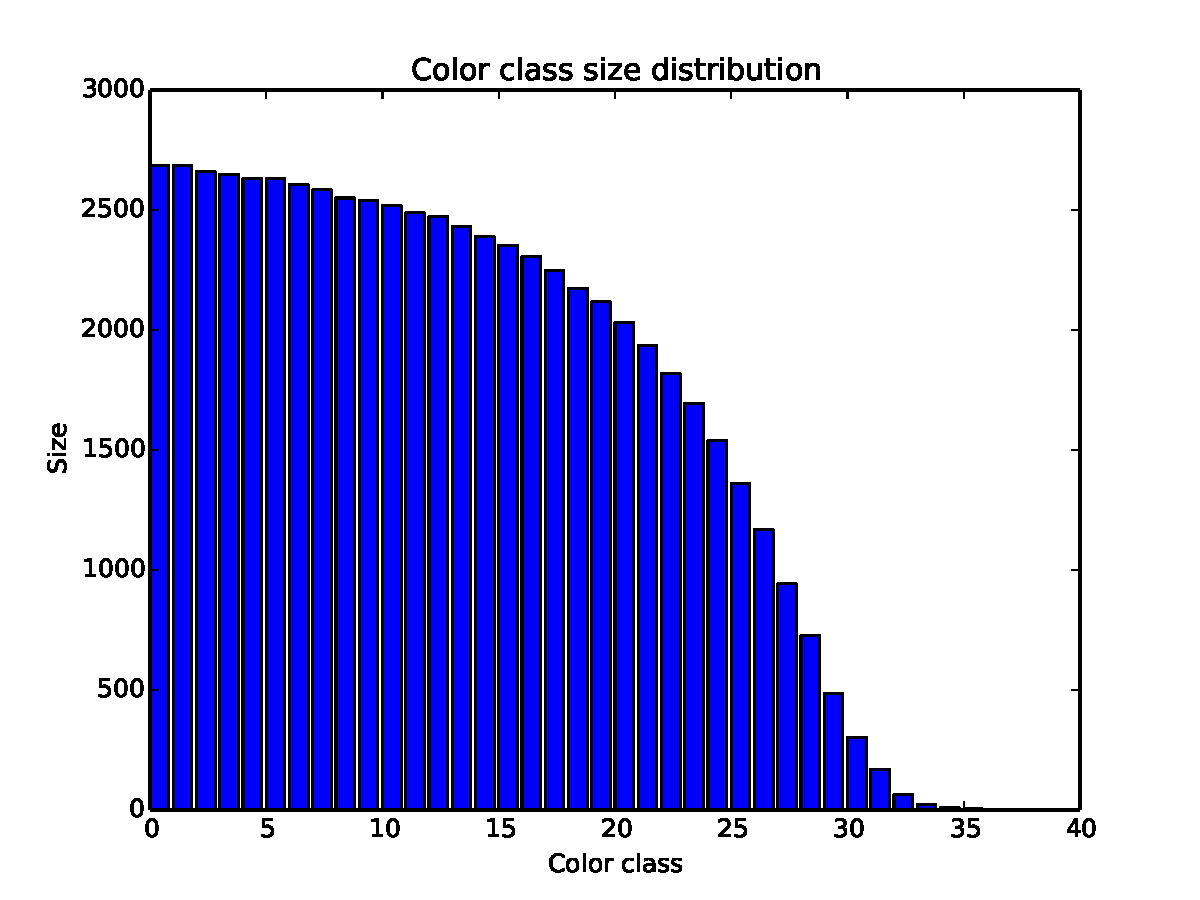
\includegraphics[width=0.9\linewidth]{figures/colors5.pdf}
	\caption{Color class sizes}
\end{subfigure}

\begin{subfigure}{0.5\textwidth}
	\centering
	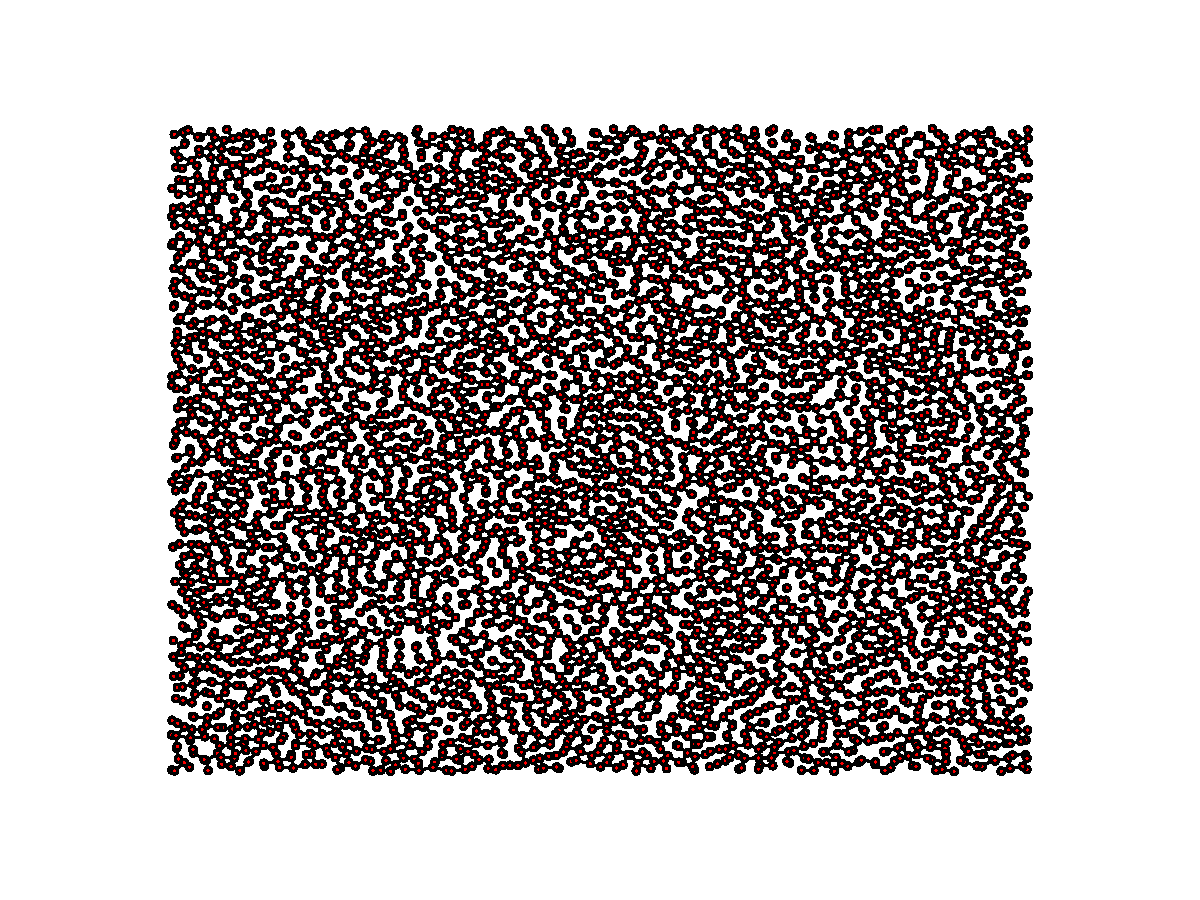
\includegraphics[width=0.9\linewidth]{figures/simplegraph5.pdf}
	\caption{Backbone 1}
\end{subfigure}%
\begin{subfigure}{0.5\textwidth}
	\centering
	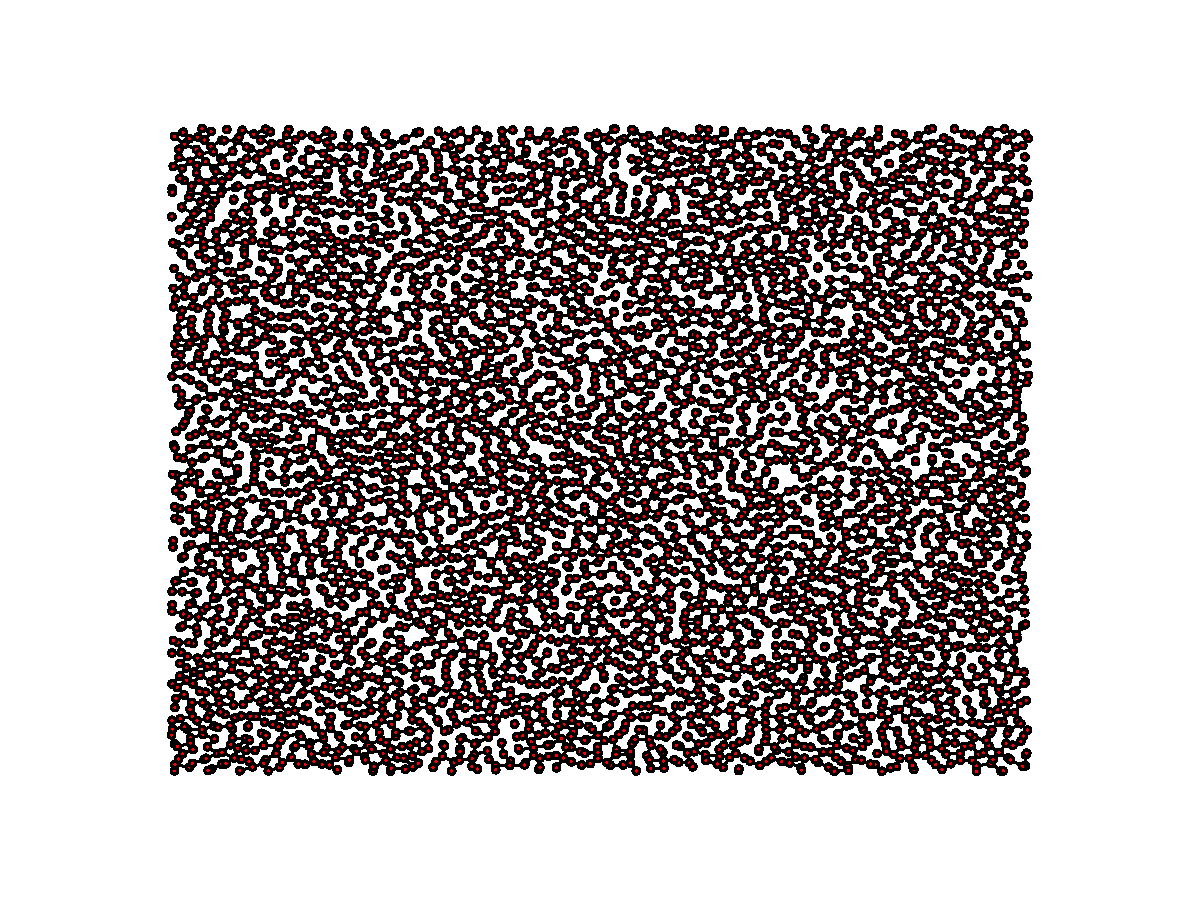
\includegraphics[width=0.9\linewidth]{figures/simplegraph51.pdf}
	\caption{Backbone 2}
\end{subfigure}
\end{figure}

\subsection{Disk, $N=4000, \Delta_{avg}=60$}
\begin{figure}[!h]
\centering
\begin{subfigure}{0.5\textwidth}
	\centering
	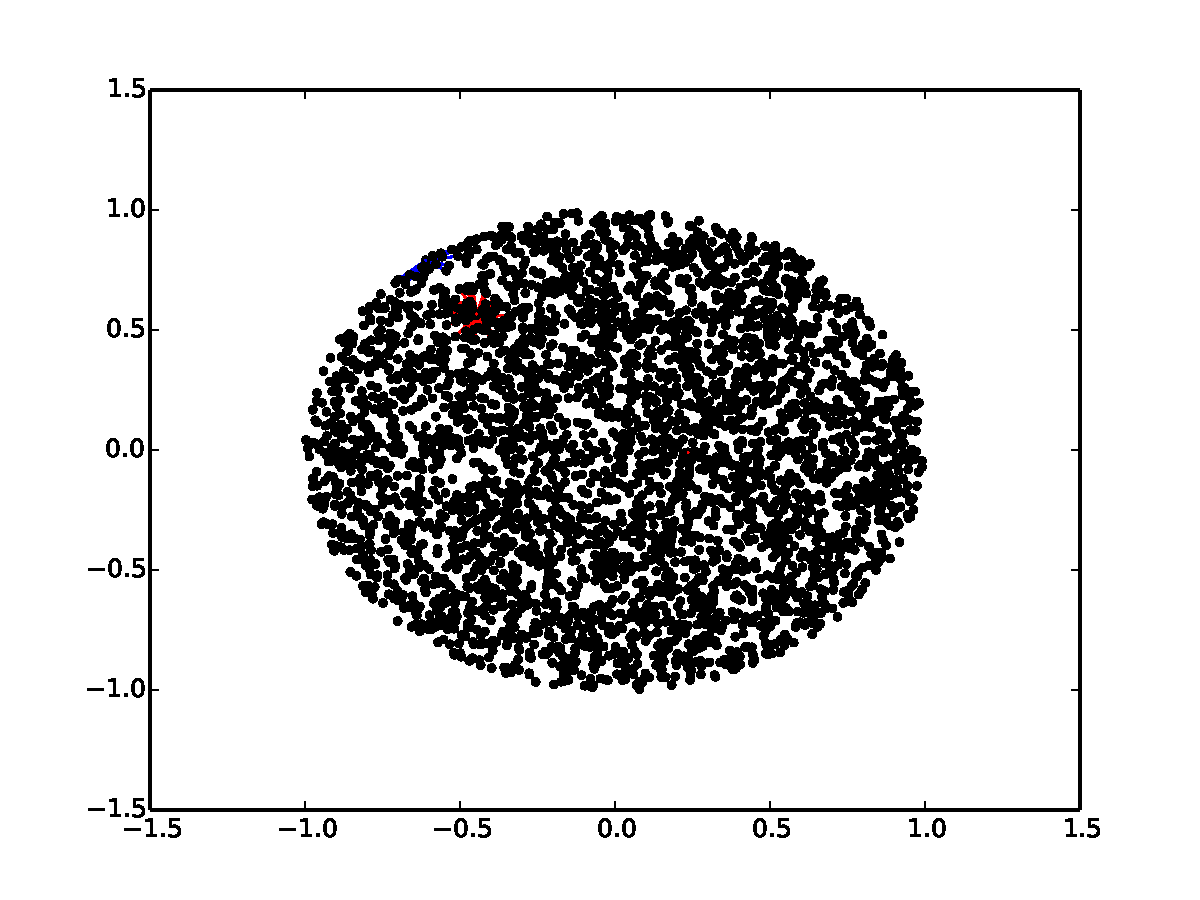
\includegraphics[width=0.9\linewidth]{figures/graph6.pdf}
	\caption{Graph}
\end{subfigure}%
\begin{subfigure}{0.5\textwidth}
	\centering
	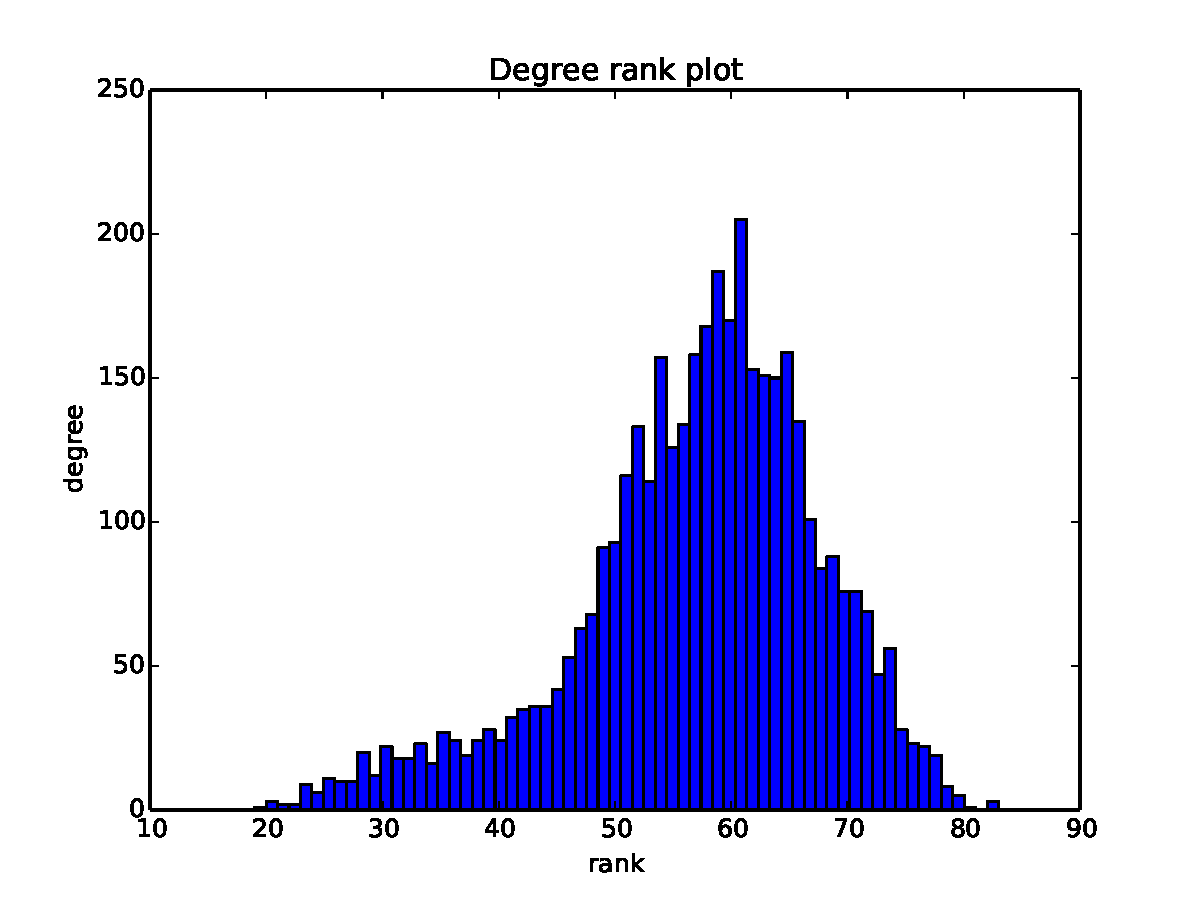
\includegraphics[width=0.9\linewidth]{figures/degrees6.pdf}
	\caption{Degree Histogram}
\end{subfigure}

\begin{subfigure}{0.5\textwidth}
	\centering
	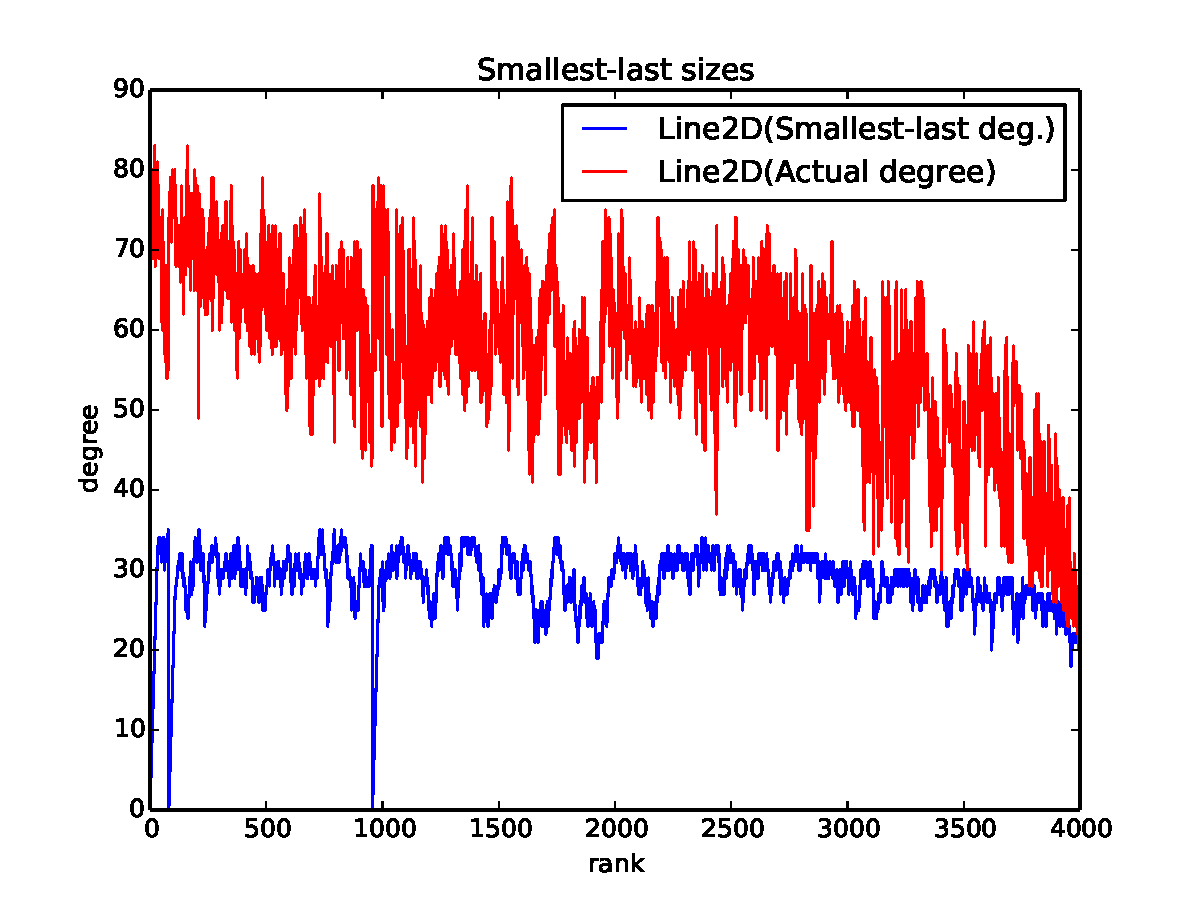
\includegraphics[width=0.9\linewidth]{figures/ordering6.pdf}
	\caption{Smallest--last degrees}
\end{subfigure}%
\begin{subfigure}{0.5\textwidth}
	\centering
	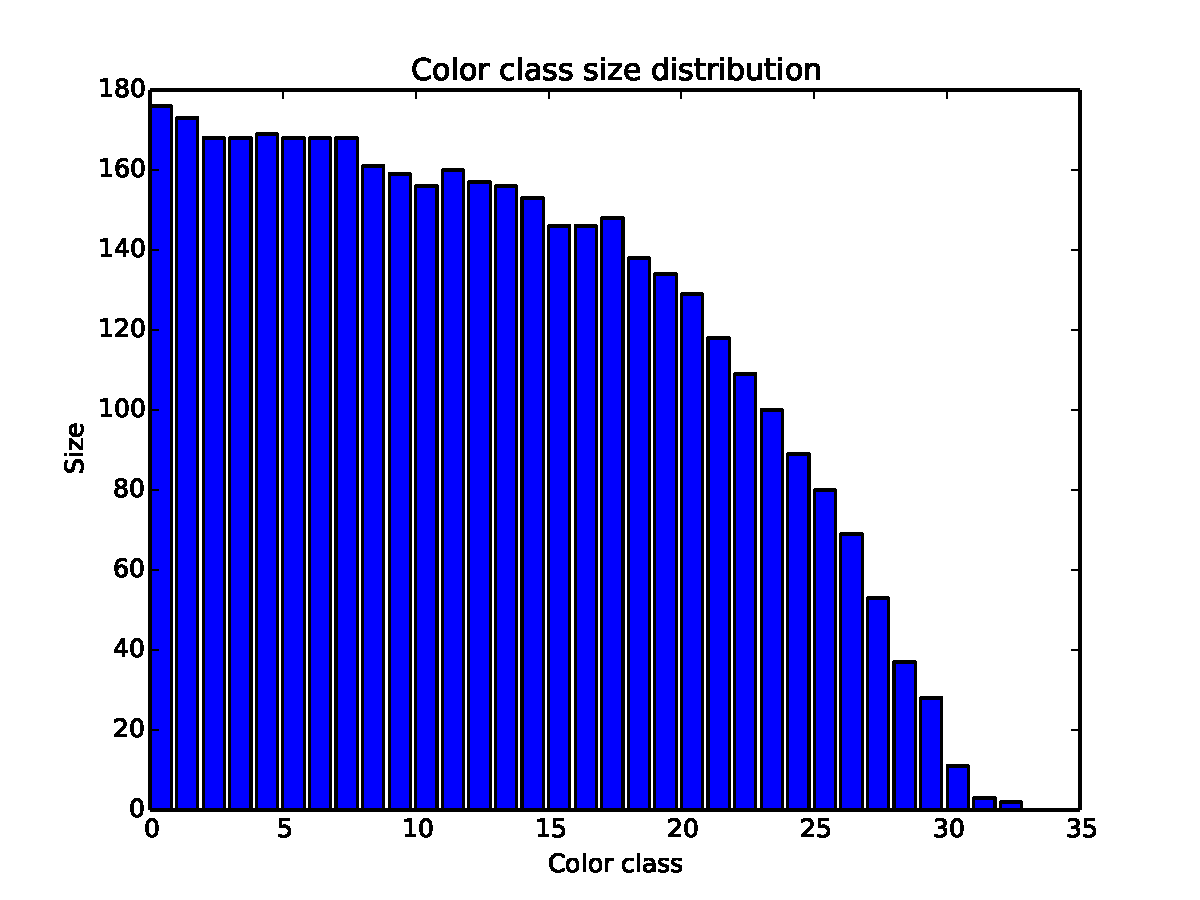
\includegraphics[width=0.9\linewidth]{figures/colors6.pdf}
	\caption{Color class sizes}
\end{subfigure}

\begin{subfigure}{0.5\textwidth}
	\centering
	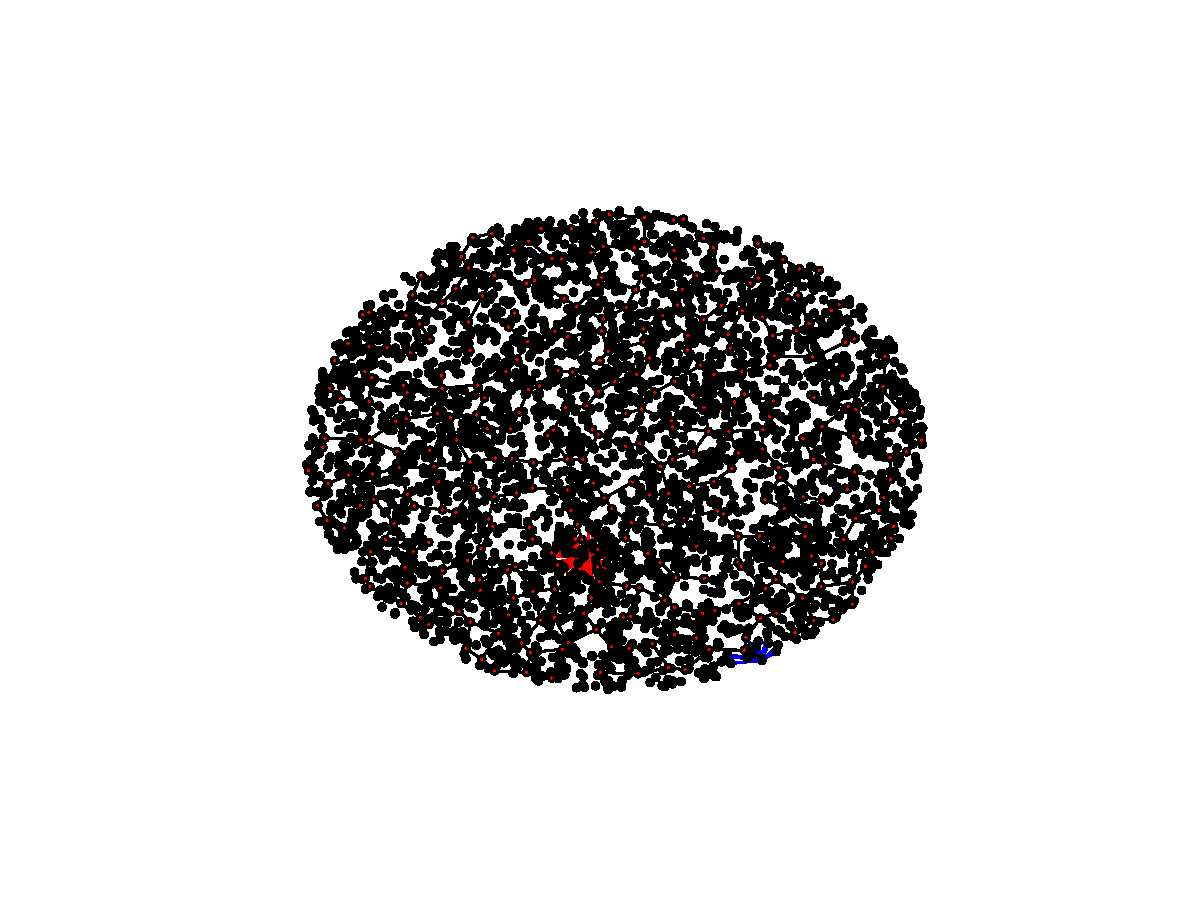
\includegraphics[width=0.9\linewidth]{figures/simplegraph6.pdf}
	\caption{Backbone 1}
\end{subfigure}%
\begin{subfigure}{0.5\textwidth}
	\centering
	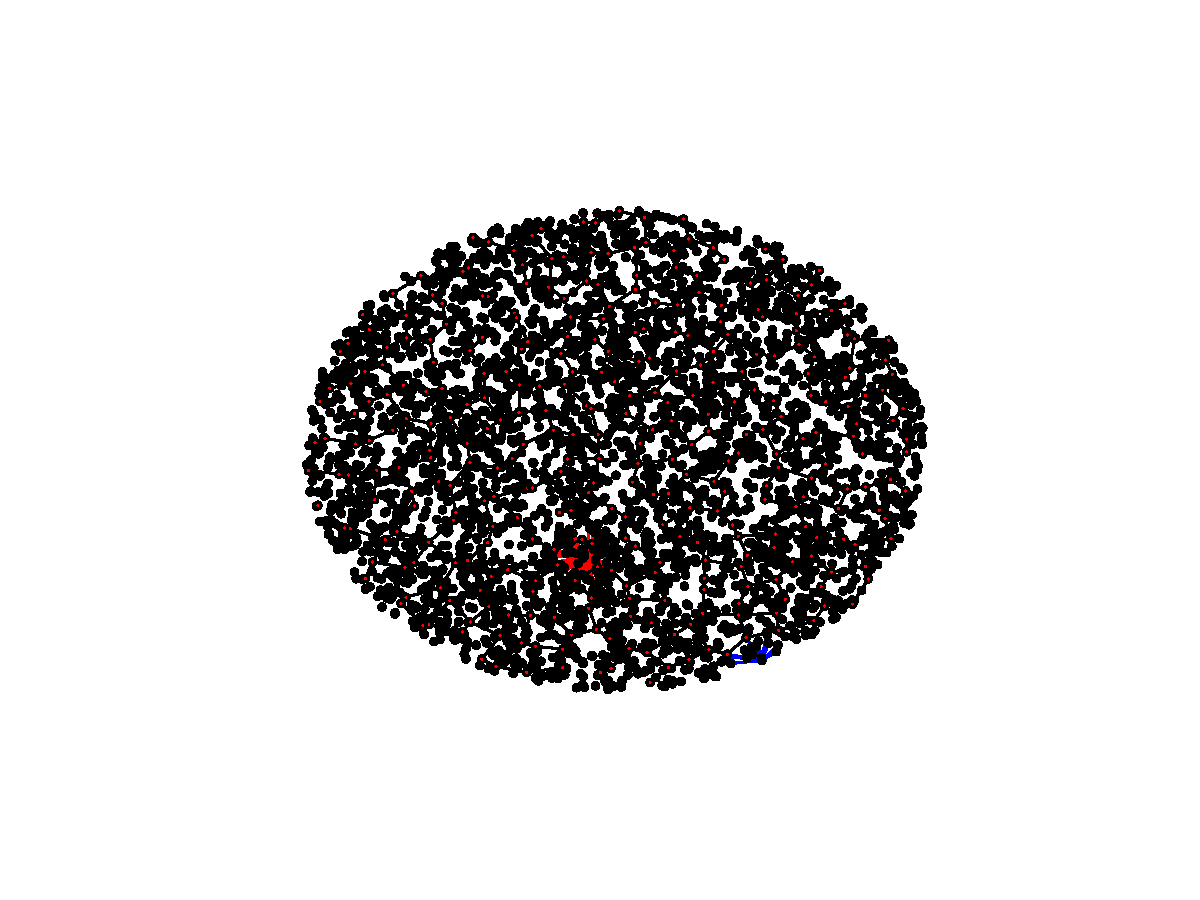
\includegraphics[width=0.9\linewidth]{figures/simplegraph61.pdf}
	\caption{Backbone 2}
\end{subfigure}
\end{figure}

\subsection{Disk, $N=4000, \Delta_{avg}=120$}
\begin{figure}[!h]
\centering
\begin{subfigure}{0.5\textwidth}
	\centering
	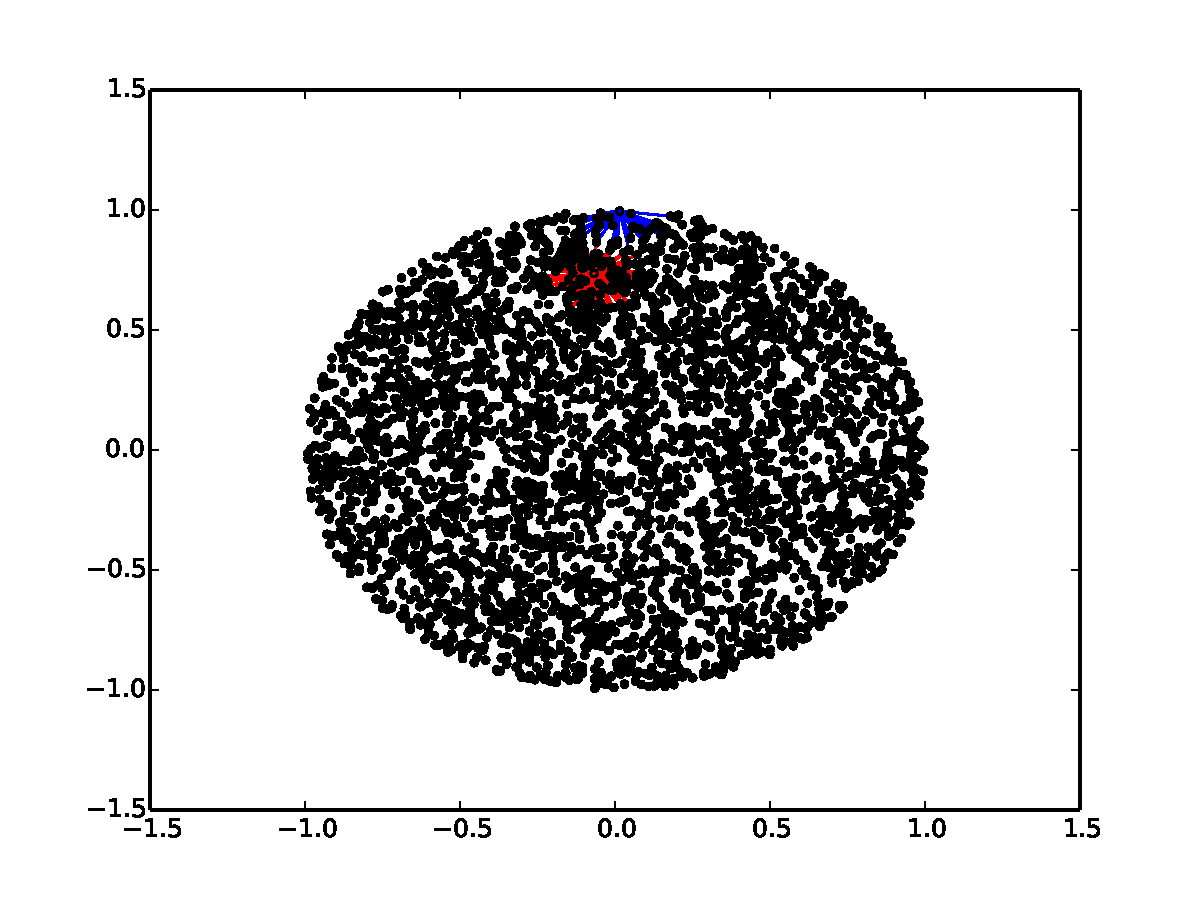
\includegraphics[width=0.9\linewidth]{figures/graph7.pdf}
	\caption{Graph}
\end{subfigure}%
\begin{subfigure}{0.5\textwidth}
	\centering
	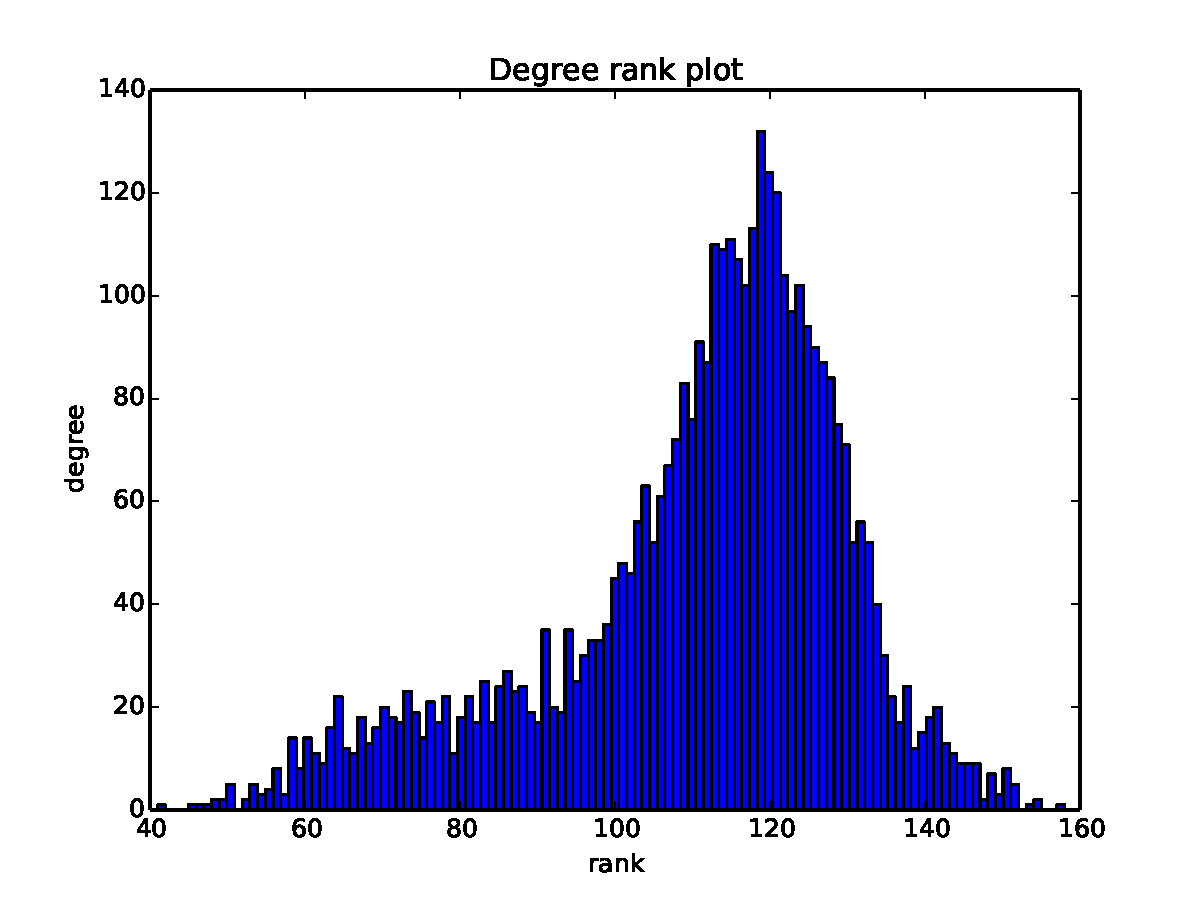
\includegraphics[width=0.9\linewidth]{figures/degrees7.pdf}
	\caption{Degree Histogram}
\end{subfigure}

\begin{subfigure}{0.5\textwidth}
	\centering
	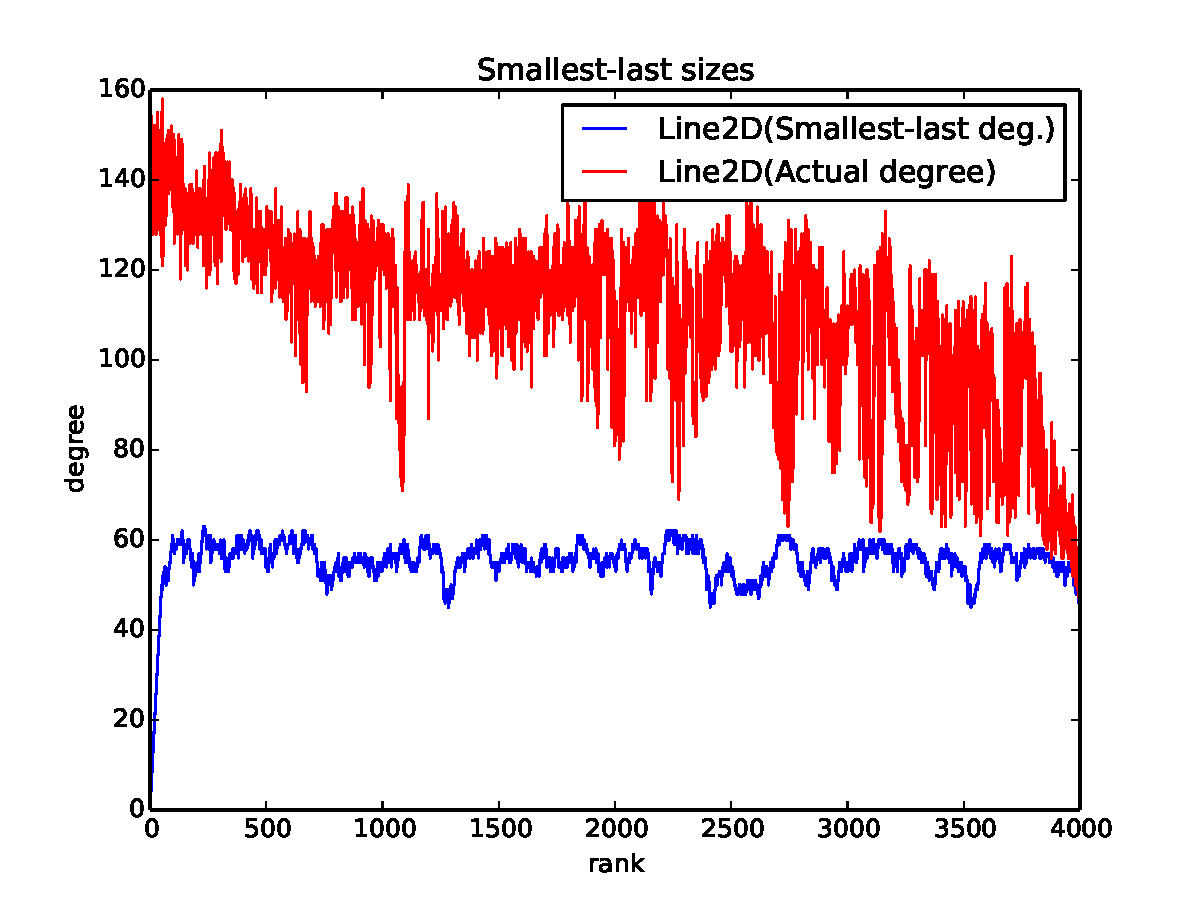
\includegraphics[width=0.9\linewidth]{figures/ordering7.pdf}
	\caption{Smallest--last degrees}
\end{subfigure}%
\begin{subfigure}{0.5\textwidth}
	\centering
	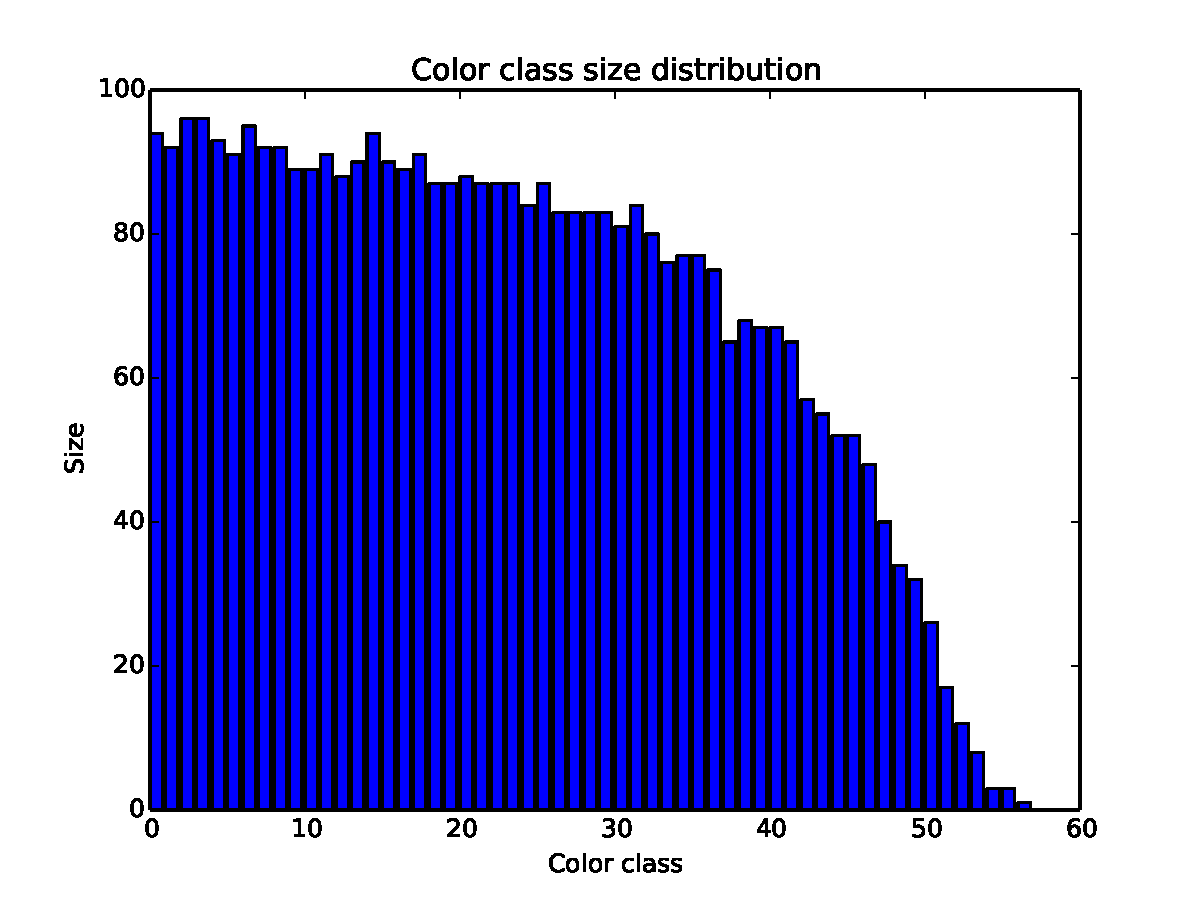
\includegraphics[width=0.9\linewidth]{figures/colors7.pdf}
	\caption{Color class sizes}
\end{subfigure}

\begin{subfigure}{0.5\textwidth}
	\centering
	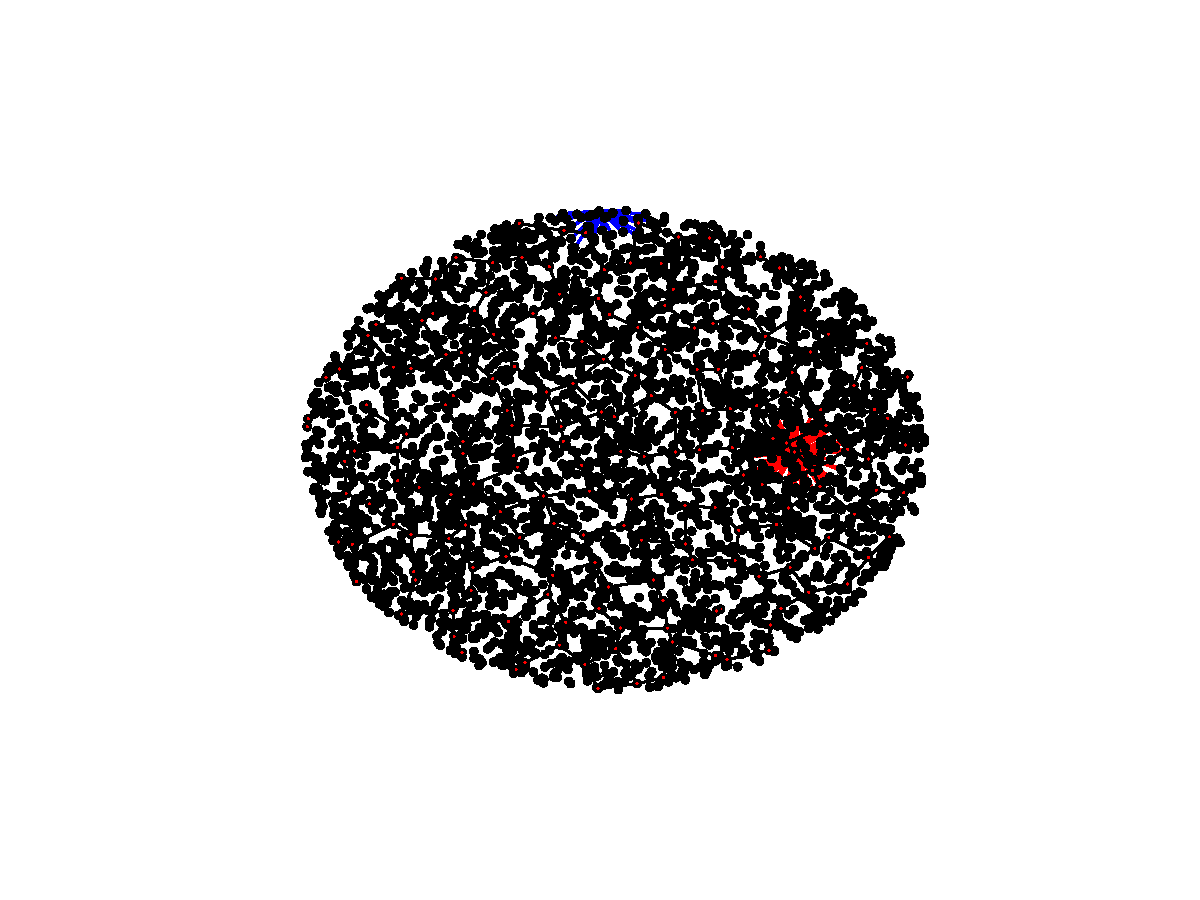
\includegraphics[width=0.9\linewidth]{figures/simplegraph7.pdf}
	\caption{Backbone 1}
\end{subfigure}%
\begin{subfigure}{0.5\textwidth}
	\centering
	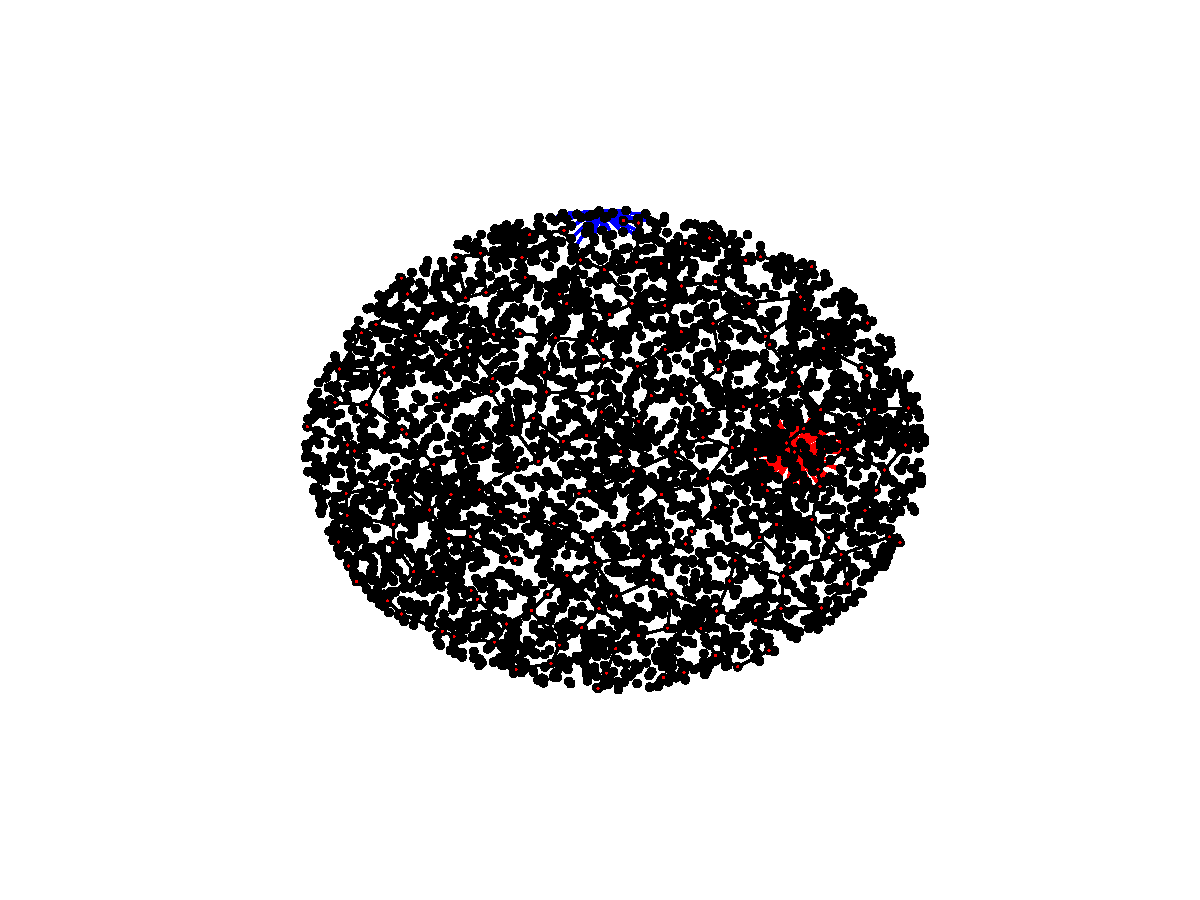
\includegraphics[width=0.9\linewidth]{figures/simplegraph71.pdf}
	\caption{Backbone 2}
\end{subfigure}
\end{figure}


\subsection{Sphere, $N=4000, \Delta_{avg}=60$}
\begin{figure}[!h]
\centering
\begin{subfigure}{0.5\textwidth}
	\centering
	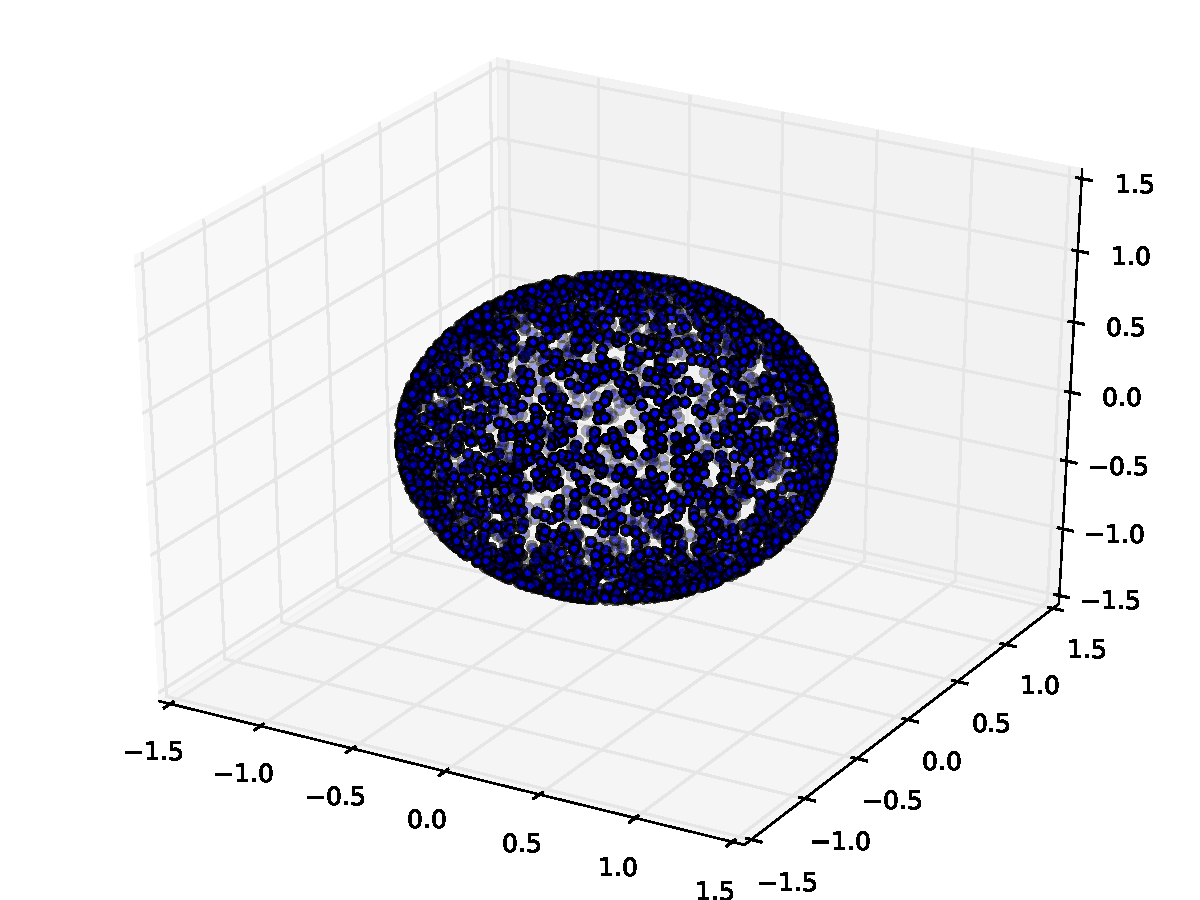
\includegraphics[width=0.9\linewidth]{figures/graph8.pdf}
	\caption{Graph}
\end{subfigure}%
\begin{subfigure}{0.5\textwidth}
	\centering
	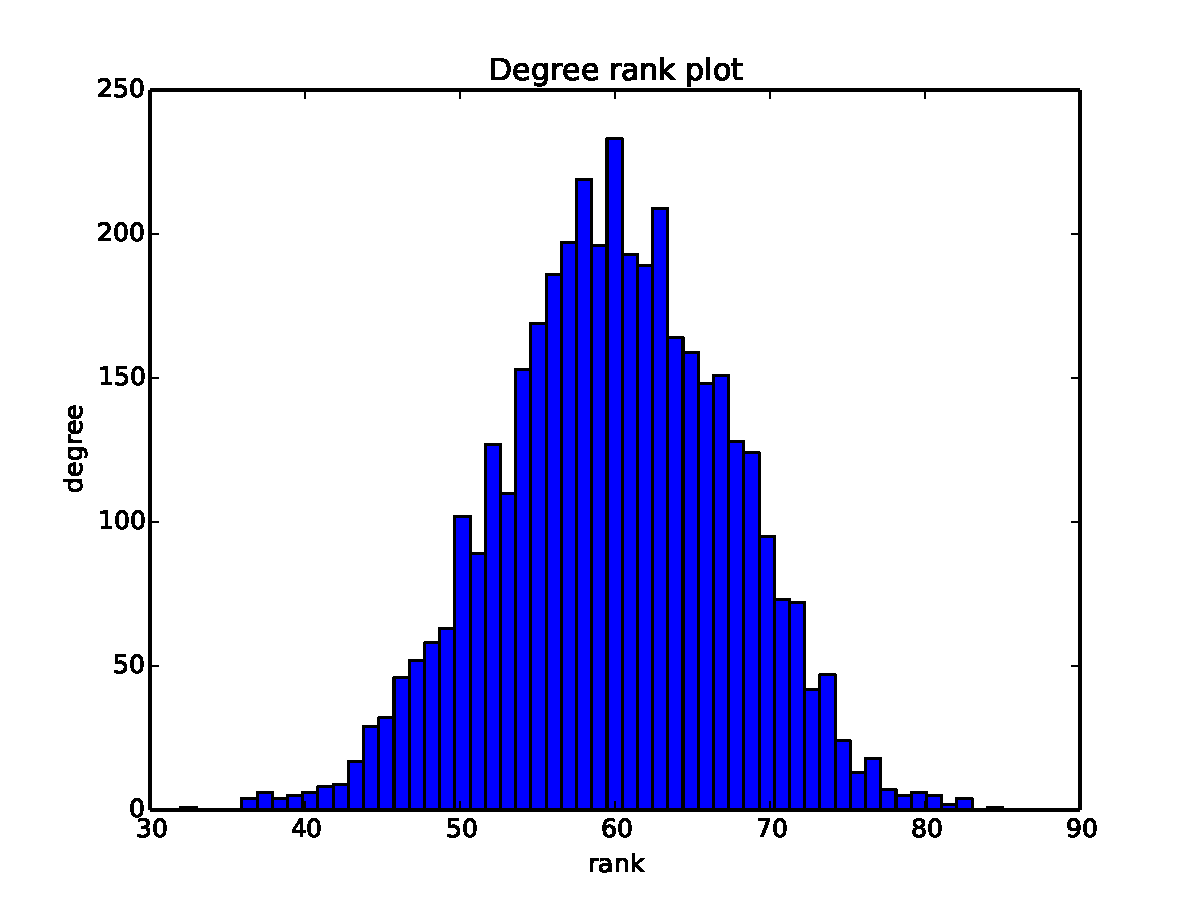
\includegraphics[width=0.9\linewidth]{figures/degrees8.pdf}
	\caption{Degree Histogram}
\end{subfigure}

\begin{subfigure}{0.5\textwidth}
	\centering
	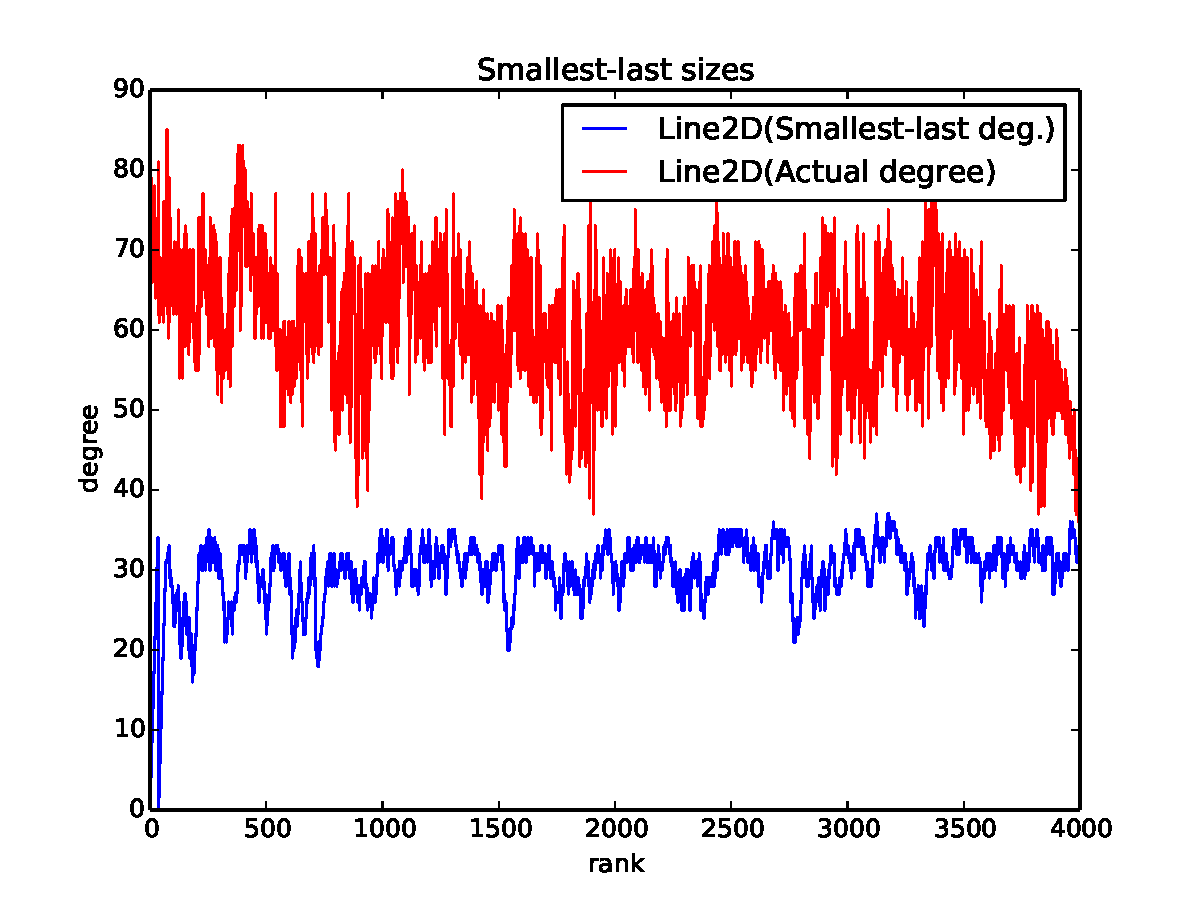
\includegraphics[width=0.9\linewidth]{figures/ordering8.pdf}
	\caption{Smallest--last degrees}
\end{subfigure}%
\begin{subfigure}{0.5\textwidth}
	\centering
	\includegraphics[width=0.9\linewidth]{figures/colors8.pdf}
	\caption{Color class sizes}
\end{subfigure}

\begin{subfigure}{0.5\textwidth}
	\centering
	\includegraphics[width=0.9\linewidth]{figures/simplegraph8.pdf}
	\caption{Backbone 1}
\end{subfigure}%
\begin{subfigure}{0.5\textwidth}
	\centering
	\includegraphics[width=0.9\linewidth]{figures/simplegraph81.pdf}
	\caption{Backbone 2}
\end{subfigure}
\end{figure}


\subsection{Sphere, $N=16000, \Delta_{avg}=120$}
\begin{figure}[!h]
\centering
\begin{subfigure}{0.5\textwidth}
	\centering
	\includegraphics[width=0.9\linewidth]{figures/graph9.pdf}
	\caption{Graph}
\end{subfigure}%
\begin{subfigure}{0.5\textwidth}
	\centering
	\includegraphics[width=0.9\linewidth]{figures/degrees9.pdf}
	\caption{Degree Histogram}
\end{subfigure}

\begin{subfigure}{0.5\textwidth}
	\centering
	\includegraphics[width=0.9\linewidth]{figures/ordering9.pdf}
	\caption{Smallest--last degrees}
\end{subfigure}%
\begin{subfigure}{0.5\textwidth}
	\centering
	\includegraphics[width=0.9\linewidth]{figures/colors9.pdf}
	\caption{Color class sizes}
\end{subfigure}

\begin{subfigure}{0.5\textwidth}
	\centering
	\includegraphics[width=0.9\linewidth]{figures/simplegraph9.pdf}
	\caption{Backbone 1}
\end{subfigure}%
\begin{subfigure}{0.5\textwidth}
	\centering
	\includegraphics[width=0.9\linewidth]{figures/simplegraph91.pdf}
	\caption{Backbone 2}
\end{subfigure}
\end{figure}


\subsection{Sphere, $N=64000, \Delta_{avg}=120$}
\begin{figure}[!h]
\centering
\begin{subfigure}{0.5\textwidth}
	\centering
	\includegraphics[width=0.9\linewidth]{figures/graph10.pdf}
	\caption{Graph}
\end{subfigure}%
\begin{subfigure}{0.5\textwidth}
	\centering
	\includegraphics[width=0.9\linewidth]{figures/degrees10.pdf}
	\caption{Degree Histogram}
\end{subfigure}

\begin{subfigure}{0.5\textwidth}
	\centering
	\includegraphics[width=0.9\linewidth]{figures/ordering10.pdf}
	\caption{Smallest--last degrees}
\end{subfigure}%
\begin{subfigure}{0.5\textwidth}
	\centering
	\includegraphics[width=0.9\linewidth]{figures/colors10.pdf}
	\caption{Color class sizes}
\end{subfigure}

\begin{subfigure}{0.5\textwidth}
	\centering
	\includegraphics[width=0.9\linewidth]{figures/simplegraph10.pdf}
	\caption{Backbone 1}
\end{subfigure}%
\begin{subfigure}{0.5\textwidth}
	\centering
	\includegraphics[width=0.9\linewidth]{figures/simplegraph101.pdf}
	\caption{Backbone 2}
\end{subfigure}
\end{figure}

\subsection{Sphere, $N=100000, \Delta_{avg}=60$}
\begin{figure}[!h]
\centering
\begin{subfigure}{0.5\textwidth}
	\centering
	\includegraphics[width=0.9\linewidth]{figures/graph40.pdf}
	\caption{Graph}
\end{subfigure}%
\begin{subfigure}{0.5\textwidth}
	\centering
	\includegraphics[width=0.9\linewidth]{figures/degrees40.pdf}
	\caption{Degree Histogram}
\end{subfigure}

\begin{subfigure}{0.5\textwidth}
	\centering
	\includegraphics[width=0.9\linewidth]{figures/ordering40.pdf}
	\caption{Smallest--last degrees}
\end{subfigure}%
\begin{subfigure}{0.5\textwidth}
	\centering
	\includegraphics[width=0.9\linewidth]{figures/colors40.pdf}
	\caption{Color class sizes}
\end{subfigure}

\begin{subfigure}{0.5\textwidth}
	\centering
	\includegraphics[width=0.9\linewidth]{figures/simplegraph40.pdf}
	\caption{Backbone 1}
\end{subfigure}%
\begin{subfigure}{0.5\textwidth}
	\centering
	\includegraphics[width=0.9\linewidth]{figures/simplegraph401.pdf}
	\caption{Backbone 2}
\end{subfigure}
\end{figure}


\subsection{Square, $N=256000, \Delta_{avg}=120$}

\begin{figure}[!h]
\centering
\begin{subfigure}{0.5\textwidth}
	\centering
	\includegraphics[width=0.9\linewidth]{figures/graph11.pdf}
	\caption{Graph}
\end{subfigure}%
\begin{subfigure}{0.5\textwidth}
	\centering
	\includegraphics[width=0.9\linewidth]{figures/degrees11.pdf}
	\caption{Degree Histogram}
\end{subfigure}

\begin{subfigure}{0.5\textwidth}
	\centering
	\includegraphics[width=0.9\linewidth]{figures/ordering11.pdf}
	\caption{Smallest--last degrees}
\end{subfigure}%
\begin{subfigure}{0.5\textwidth}
	\centering
	\includegraphics[width=0.9\linewidth]{figures/colors11.pdf}
	\caption{Color class sizes}
\end{subfigure}

\begin{subfigure}{0.5\textwidth}
	\centering
	\includegraphics[width=0.9\linewidth]{figures/simplegraph11a.pdf}
	\caption{Backbone 1}
\end{subfigure}%
\begin{subfigure}{0.5\textwidth}
	\centering
	\includegraphics[width=0.9\linewidth]{figures/simplegraph11a.pdf}
	\caption{Backbone 2}
\end{subfigure}
\end{figure}

\subsection{Square, $N=1000, \Delta_{avg}=200$}

\begin{figure}[!h]
\centering
\begin{subfigure}{0.5\textwidth}
	\centering
	\includegraphics[width=0.9\linewidth]{figures/graph50.pdf}
	\caption{Graph}
\end{subfigure}%
\begin{subfigure}{0.5\textwidth}
	\centering
	\includegraphics[width=0.9\linewidth]{figures/degrees50.pdf}
	\caption{Degree Histogram}
\end{subfigure}

\begin{subfigure}{0.5\textwidth}
	\centering
	\includegraphics[width=0.9\linewidth]{figures/ordering50.pdf}
	\caption{Smallest--last degrees}
\end{subfigure}%
\begin{subfigure}{0.5\textwidth}
	\centering
	\includegraphics[width=0.9\linewidth]{figures/colors50.pdf}
	\caption{Color class sizes}
\end{subfigure}

\begin{subfigure}{0.5\textwidth}
	\centering
	\includegraphics[width=0.9\linewidth]{figures/simplegraph50.pdf}
	\caption{Backbone 1}
\end{subfigure}%
\begin{subfigure}{0.5\textwidth}
	\centering
	\includegraphics[width=0.9\linewidth]{figures/simplegraph501.pdf}
	\caption{Backbone 2}
\end{subfigure}
\end{figure}

\end{document} 
